\documentclass[11pt]{article}
\usepackage[T1]{fontenc}
\usepackage{lmodern}
\usepackage[margin=1in]{geometry}
\usepackage{amsmath,amssymb,amsthm,mathtools,mathrsfs}
\usepackage{microtype,enumitem,booktabs,array,graphicx}
\usepackage{tikz}
\usetikzlibrary{arrows.meta,patterns,positioning,calc}
\usepackage{xcolor}
\definecolor{linkblue}{RGB}{28,75,118}
\usepackage[colorlinks=true,linkcolor=linkblue,citecolor=linkblue,urlcolor=linkblue]{hyperref}
\usepackage[nameinlink,capitalise,noabbrev]{cleveref}
\pdfinfoomitdate=1
\pdftrailerid{}
\pdfsuppressptexinfo=15
\numberwithin{equation}{section}
\newtheorem{theorem}{Theorem}[section]
\newtheorem{lemma}[theorem]{Lemma}
\newtheorem{proposition}[theorem]{Proposition}
\newtheorem{corollary}[theorem]{Corollary}
\theoremstyle{definition}
\newtheorem{definition}[theorem]{Definition}
\theoremstyle{remark}
\newtheorem{remark}[theorem]{Remark}
\newcommand{\R}{\mathbb R}
\newcommand{\C}{\mathbb C}
\newcommand{\Z}{\mathbb Z}
\newcommand{\N}{\mathbb N}
\newcommand{\T}{\mathbb T}
\newcommand{\E}{\mathbb E}
\newcommand{\PP}{\mathbb P}
\newcommand{\dd}{\,\mathrm d}
\newcommand{\one}{\mathbf 1}
\newcommand{\norm}[1]{\left\lVert#1\right\rVert}
\newcommand{\abs}[1]{\left\lvert#1\right\rvert}
\DeclareMathOperator{\supp}{supp}
\DeclareMathOperator{\dist}{dist}
\DeclareMathOperator{\diam}{diam}
\DeclareMathOperator{\tr}{tr}
\DeclareMathOperator{\diag}{diag}
\DeclareMathOperator{\rank}{rank}
\DeclareMathOperator{\Law}{Law}
\setlength{\emergencystretch}{1.5em}
\hypersetup{pdftitle={Pure-Point Spectrum for the Two-Dimensional Anderson Model at Every Positive Disorder},pdfauthor={OpenAI}}
\title{Pure-Point Spectrum for the Two-Dimensional\\Anderson Model at Every Positive Disorder}
\author{OpenAI}
\date{September 23, 2026}
\begin{document}
\maketitle
\begin{abstract}
For each fixed positive disorder strength, we prove that the nearest-neighbor
Anderson operator on the square lattice with independent uniform site
potentials almost surely has pure-point spectral type throughout its spectrum.
This resolves the pure-point assertion of the two-dimensional Anderson
localization conjecture for the uniform single-site law.
\end{abstract}
\section{Introduction}

Let $h>0$ and let $(v_x)_{x\in\Z^2}$ be independent random variables,
each uniform on $[-h,h]$. We consider the bounded self-adjoint operator
\begin{equation}\label{setup:model}
 (H_v u)(x)=\sum_{\abs{y-x}_1=1}u(y)+v_xu(x)
 \qquad\text{on }\ell^2(\Z^2).
\end{equation}
Thus $v_x=h\omega_x$ in the usual notation with $\omega_x$ uniform on
$[-1,1]$. Pure-point spectral type means that the closed span of the
eigenvectors is the entire Hilbert space; it does not mean that every
point of the spectrum is an eigenvalue.

The planar spectral localization problem asks whether this pure-point
conclusion holds throughout the spectrum for every nonzero width of the
uniform distribution \cite[Example~2.1 and Problem~2]{Simon2000}.
We prove that it does.

\begin{theorem}\label{main:theorem}
For each fixed $h>0$, almost surely $H_v$ has pure-point spectral type,
admits a complete orthonormal eigenbasis, and has spectrum
\[
 \sigma(H_v)=[-4-h,4+h].
\]
Its eigenvalues are dense in this interval. The probability-one event
in this statement is allowed to depend on $h$.
\end{theorem}

The conclusion includes arbitrarily weak nonzero disorder and the entire
spectrum. It resolves the pure-point assertion of the two-dimensional
Anderson localization conjecture for a uniform single-site distribution,
as formulated in \cite[Problem~2]{Simon2000}. An arbitrary nondegenerate
uniform interval reduces to the centered interval above by subtracting
its midpoint from the operator. We do not assert one probability-one
event for all disorder strengths, a bound uniform in energy, or a
dynamical-localization theorem.

\subsection*{Context and scope}
Anderson introduced random site energies as a mechanism for suppressing
quantum transport, motivated by spin diffusion and impurity conduction
\cite{Anderson1958}. His discussion includes a flat single-site
distribution and nearest-neighbor hopping, although the original
physical argument is not a modern proof of the spectral assertion
considered here. The conductance-scaling theory of Abrahams, Anderson,
Licciardello and Ramakrishnan predicts the absence of true metallic
behavior in two dimensions
\cite{AbrahamsAndersonLicciardelloRamakrishnan1979}. That physical
prediction is distinct from an almost-sure spectral-type theorem.
Simon's formulation isolates the latter question; his diffusion
problem is listed separately \cite{Simon2000}.

Rigorous multidimensional localization theory developed several
complementary mechanisms.
Fr\"ohlich and Spencer's multiscale analysis gave Green-function decay
and vanishing Kubo diffusion in large-disorder or appropriate
extreme-energy regimes \cite{FrohlichSpencer1983}. Their 1983
conclusions were explicitly distinguished from a complete pure-point
decomposition. Fr\"ohlich, Martinelli, Scoppola and Spencer subsequently
established pure-point spectrum with exponentially decaying
eigenfunctions for independent identically distributed diagonal
potentials with a bounded density in sufficiently large-disorder and suitable tail-energy
regimes \cite{FMSS1985}. Delyon, L\'evy and Souillard also obtained
multidimensional spectral localization in large-disorder or large-energy
regimes \cite{DelyonLevySouillard1985}. The passage from fixed-energy
Green-function information to a complete spectral decomposition is a
substantive step, not an automatic consequence of decay outside an
exceptional set of energies.

Aizenman and Molchanov developed the fractional-moment approach,
obtaining localization at large disorder and at extreme energies under
suitable hypotheses on the conditional single-site distributions,
including absolute continuity and regularity
\cite{AizenmanMolchanov1993}. This method supplies important ancestry for
our use of fractional Green-function moments, but its established
regimes do not by themselves yield the all-disorder, all-energy
assertion above. Spectral-edge results also have a different scope.
Ding and Smart proved localization near an edge for the two-dimensional
Bernoulli model and observed that their proof extends to bounded
nontrivial iid laws
\cite{DingSmart2020}; Hurtado extended edge-localization and
unique-continuation methods to independent, not necessarily identically
distributed uniformly bounded potentials with uniformly positive variance
\cite{Hurtado2026}. The latter
localization theorems remain restricted to a bottom interval, even
though their distributional assumptions are broader.

Weak-disorder transport on long finite scales poses another, compatible
question. Black, Drogin and Hern\'andez obtain quantitative time-averaged
diffusion, resolvent and finite-volume eigenfunction results for
Gaussian iid potentials on disorder-dependent scales
\cite{BlackDroginHernandez2025}.
These weak-coupling limits neither imply nor contradict pure-point
spectral type at every fixed positive disorder for the uniform law.
The present assertion concerns that fixed-disorder spectral type; it
does not assert exponential eigenfunction decay or dynamical localization.

The final spectral step follows the rank-one mechanism of Simon and
Wolff \cite{SimonWolff1986}. Its input is a suitable inverse-square
spectral integral, equivalently a square-summable resolvent column, for
almost every configuration and energy. Averaging over the independent
site value transfers this information to the random spectral measure.
We prove the required averaging and spectral readout explicitly; the
main work is to obtain their fixed-energy input under the true uniform
product law at arbitrary disorder.

\subsection*{The proof mechanism}
Fix $h>0$ and an interior real energy $E$. In \cref{mat:section}, we introduce absorbing
diagonal terms in finite tori and their associated input and output
channels, called ports. Squared scattering amplitudes define a
Dirichlet energy on port data: if $S_{ja}$ is the scattering amplitude
from port $a$ to port $j$ and $f$ is real data on the ports, the energy is
\[
 \mathcal Q_S(f)=\frac12\sum_{a,j}|S_{ja}|^2|f_j-f_a|^2.
\]
A Cauchy-distributed real closing value
would remove a port with a favorable averaged energy comparison. The
bounded physical distribution requires a truncated version and a
relative estimate for its error.

The first main ingredient is a family of rare resonant cells
(\cref{sec:resonant,sec:impedance,sec:transmission}). Their
conditional law is embedded in the original product measure by an
acceptance likelihood; the true potentials remain independent uniforms
before conditioning. The construction gives a weighted boundary
impedance estimate uniform in arbitrary passive exterior data, including
weakly coupled missing boundary directions. It also gives a transmission
lower bound strong enough to make the closing error small relative to
the transmission itself. These estimates, together with an upper
envelope over adaptive interior configurations, are useful beyond a
single prescribed environment.

The second ingredient is a comparison along a hierarchy of increasingly
sparse ports (\cref{sec:hierarchy}). A parent-cell alternative controls the apparent singularity
at the end of each thinning interpolation. Local generic observation,
followed by path estimates, supplies screening at every fixed starting
stage (\cref{sec:screening}). For a fixed starting level $n$, let $d_n$
be the infinite-volume limit of the expected sum of squared port-to-port
distances, weighted by $|S_{ja}|^2$ and divided by twice the torus area.
These quantities measure the scattering energy of affine coordinate
data. The torus side tends to infinity with $n$ fixed to define $d_n$;
only afterwards does the thinning comparison give a finite limit $d$
as $n$ tends to infinity.

The dimension enters decisively in forcing $d=0$ (\cref{sec:vanishing}).
An adaptive modification of affine data first makes a local affine
first-variation trace small in expectation. Separately, a logarithmic voltage profile separates
retained interior ports from an annulus of very weak probes at
arbitrarily small two-dimensional capacity cost. If $d>0$,
an analytic test of the scattering matrix has a nonzero value at the
center of the disk. Support-preserving shifts of the true potentials
and the thinning comparison make its boundary moments arbitrarily small,
contradicting submean. Dimension-free weak integral bounds prevent the
number of ports from spoiling this argument.

Finally, vanishing affine energy is upgraded to a fixed-real-energy
fractional-moment estimate for the true finite-torus Green function
(\cref{sec:bootstrap}).
Buffered probe barriers, conditional estimates under transmission
weights, and resampling of disjoint regions close a contraction uniform
over the allowed masks. The infinite-volume conclusion then follows
from the spectral theorem, Fubini, and rank-one averaging
(\cref{sec:spectral}). The property
to which Fubini is applied belongs to the true operator, so no common
auxiliary construction measurable in energy is needed.

The proof keeps these roles separate: the rare laws prove local
comparisons, fixed-stage screening controls limits, two-dimensional
capacity makes the limit vanish, and spectral averaging converts
fixed-energy information to spectral type.

\section{Finite volumes and conventions}\label{setup:conventions}

Throughout the local and multiscale arguments, fix
\begin{equation}\label{setup:fixed-energy}
 h>0,\qquad -4-h<E<4+h.
\end{equation}
All constants and auxiliary choices may depend on this pair. Their
dependence on the varying geometric scales, exterior data and masks is
specified in each assertion. Uniformity in $E$ is neither assumed nor
needed for \cref{main:theorem}.

For integer $l\ge0$, put $b_l=3^l$. The global finite volume is the square
torus
\[
 \mathbb T_N^2=(\Z/b_N\Z)^2,
\]
with the periodic nearest-neighbor adjacency and independent uniform
potentials on its sites. Its area is $b_N^2$. Distances are shortest
coordinate distances on this torus, using the maximum norm unless a
different norm is displayed. We write
\[
 \Lambda_r(x)=\{y:\abs{y-x}_\infty\le r\}.
\]
All local constructions are used with the torus sufficiently large to
contain the required neighborhoods without ambiguity. Dirichlet
restrictions mean deletion of the hopping bonds leaving the indicated
physical site set.

The physical disorder is always the product law of the true variables
$v_x$. Auxiliary selectors, acceptance uniforms, offsets and thinning
marks will be introduced explicitly. Conditioning on a rare event can
change the law within one cell; it never changes this unconditional
physical law. An expectation refers to the sampling and conditioning
specified in its statement.

Site and port spaces are complexified finite-dimensional Euclidean
spaces. A superscript $\top$ denotes transpose, not adjoint; a superscript
$*$ denotes adjoint. Bases used for coordinate projections and their
subspaces are real orthonormal bases. We use
\[
 \operatorname{Im}D=\frac{D-D^*}{2i},\qquad
 \operatorname{Re}D=\frac{D+D^*}{2}.
\]
Unless otherwise indicated, a norm is the Euclidean or induced operator
norm. Hilbert--Schmidt and trace norms carry subscripts $\mathrm{HS}$
and $1$. Coordinate projections may be identified with their ranges.
Symbols used for local blocks are reset when the local matrix is defined.

A real reference potential may replace a true potential only at a site
carrying an open cell port. Closing that port restores the true value.
The matrix $H^\#$ denotes the real symmetric operator with the current
reference values. Artificial probes, introduced in the next section, do
not alter real reference values. Several ports may share a physical site;
their columns are kept distinct.

In bounds for a cell of size $L$, the notation $\operatorname{poly}(L)$
means a quantity bounded by $C(1+L)^C$ for fixed constants. The constants
may depend on the previously fixed cell-design parameters, including
the corner-box width exponent, but not on the exterior matrix, exterior
volume, exterior source, or allowed probe mask. The ordering of design
parameters is part of each construction. Expressions
$\exp(L^{O(1)})$ have the corresponding interpretation. A statement
requiring sufficiently large $L$ is applied only after its fixed design
parameters have been chosen.

We will repeatedly distinguish the following orders of choice. The
disorder and energy are fixed first. Local design constants are fixed
before the cell scale is enlarged. For global limits a starting level
$n$ is fixed before observation and approximation constants are chosen;
a later level $m$ can then be increased to exceed all those thresholds,
and the torus level $N$ is increased last. No rate uniform in $n$ is
implicit in this convention.

\section{Scattering matrices and analytic estimates}
\label{mat:section}

All matrices in this section are finite dimensional. A port at a physical
site $x$, of strength $\sigma>0$, is represented by the column
$\sqrt{\sigma}\,e_x$. In the matrix $Y$ of these columns, rows index
physical sites and columns index ports; several distinct ports may be
attached to the same site. For a real symmetric matrix
$H^\#$ and a real energy $E$, set
\begin{equation}
  \mathscr L=H^\#-E-iYY^\top,\qquad
  G=\mathscr L^{-1},\qquad
  S=\one+2iY^\top GY.
  \label{mat:response}
\end{equation}
The entry $S_{ja}$ is the scattering amplitude from input port $a$ to
output port $j$. The physical matrix $H^\#$ may differ from the true
Hamiltonian by real diagonal changes at sites carrying ports. We call these changes
\emph{reference potentials}. They may depend on the true potentials.

Absorption bounds the response between ports even when the full inverse
$G$ is large. Closing ports removes their absorptions and changes real
diagonal values; we express this operation as a rational family of
scattering matrices and compare its energies after averaging the closing
values.

\subsection{Invertibility, absorption, and Schur complements}

The inverses in \Cref{mat:response} exist almost surely under any
absolutely continuous joint law of the true site potentials. Indeed, if
$\mathscr L u=0$, taking the imaginary part of $u^*\mathscr L u$ gives
$Y^\top u=0$. Thus $u$ vanishes at every port site, so restoring the true
diagonal entries leaves its equation unchanged: $(H-E)u=0$. For a fixed
finite site set, $\det(H-E)$ is a polynomial in its true diagonal
variables whose coefficient of their full product is one. It is not
identically zero. A nonzero polynomial has a Lebesgue-null zero set,
as follows by induction on the number of variables and one-variable
slicing. This proves the assertion even when the port set and reference
potentials depend on those variables. The same argument applies to
deterministic restrictions to physical sites. We always discard the
resulting null exceptional sets when forming such inverses.

A matrix $D$ is \emph{passive} if $\operatorname{Im}D\le0$, with the
Hermitian imaginary part fixed in \cref{setup:conventions}. The absorption
identities below apply to any real rectangular $Y$, including real
coordinate or subspace inclusions.

\begin{lemma}[Absorption identities]\label{mat:ward}
Suppose $\mathscr L$ is invertible and
$W=-\operatorname{Im}\mathscr L\ge YY^\top$. Then
\begin{align}
  \operatorname{Im}G&=G^*WG=GWG^*,
  \label{mat:ward-identity}\\
  \norm{Y^\top GYa}^2
    &\le \operatorname{Im}(a^*Y^\top GYa),
  \qquad \norm{Y^\top GY}\le1.
  \label{mat:ward-contraction}
\end{align}
For the physical system in \Cref{mat:response}, $S$ is symmetric and
unitary. If $\mathscr L$ is complex symmetric and passive, each defined
Schur complement is complex symmetric and passive. An absorption lower
bound supported on retained coordinates persists in the Schur complement.
\end{lemma}

\begin{proof}
The inverse difference identities give
\[
  G-G^*=G^*(\mathscr L^*-\mathscr L)G
        =G(\mathscr L^*-\mathscr L)G^*,
\]
which proves \Cref{mat:ward-identity}. Consequently, with $K=Y^\top GY$,
\[
 \norm{Ka}^2
 \le a^*Y^\top G^*WGY a
 =\operatorname{Im}(a^*Ka)
 \le\norm a\,\norm{Ka}.
\]
This proves \Cref{mat:ward-contraction}. In the physical case $W=YY^\top$,
we have $\operatorname{Im}K=K^*K$ and hence
\[
 (\one+2iK)^*(\one+2iK)
   =\one-4\operatorname{Im}K+4K^*K=\one.
\]
Since the matrix is square, it is unitary. Symmetry follows from
$\mathscr L^\top=\mathscr L$ and the fact that $Y$ is real.

For the Schur assertion, write a symmetric matrix in blocks as
\[
 D=\begin{pmatrix}D_{11}&C\\ C^\top&D_{22}\end{pmatrix},\qquad
 D_{\mathrm{eff}}=D_{11}-CD_{22}^{-1}C^\top.
\]
For a vector $v$ on the retained coordinates, extend it to
$\widetilde v=(v,-D_{22}^{-1}C^\top v)$. Then
\[
 D\widetilde v=(D_{\mathrm{eff}}v,0),\qquad
 \widetilde v^*D\widetilde v=v^*D_{\mathrm{eff}}v.
\]
Taking imaginary parts proves passivity. If
$-\operatorname{Im}D\ge\diag(W_0,0)$, the same identity gives
$-\operatorname{Im}D_{\mathrm{eff}}\ge W_0$. Symmetry is immediate from
the displayed Schur formula.
\end{proof}

We will also use the elementary kernel consequence of passivity: if
$Du=0$ and $D$ is passive, then
$\operatorname{Im}D\,u=\operatorname{Re}D\,u=0$. Indeed, the nonnegative
matrix $-\operatorname{Im}D$ has zero quadratic form on $u$, so it
annihilates $u$; the assertion about the real part follows from $Du=0$.

\subsection{Closing ports and comparing energies}

Symmetry and unitarity make $\abs{S_{ja}}^2$ symmetric nonnegative
weights with unit row sums. For real scalar or real Euclidean-vector
data $f$ on the ports, their Dirichlet energy and its single-port
contribution are
\begin{equation}
 \mathcal Q_S(f)=\frac12\sum_{a,j}\abs{S_{ja}}^2\abs{f_j-f_a}^2,
 \qquad
 \mathcal M_a(f)=\sum_j\abs{S_{ja}}^2\abs{f_j-f_a}^2.
 \label{mat:energies}
\end{equation}
For scalar data, writing $F=\diag(f)$, unitarity gives
\begin{equation}
 \mathcal Q_S(f)=\tr(F^2-FSFS^*).
 \label{mat:energy-trace}
\end{equation}
For vector data, one sums this identity over real components.

\begin{lemma}[Common-phase closure]\label{mat:closure}
Partition the ports into retained ports and a set $C$ to be closed, and
write
\[
 S=\begin{pmatrix}A&T\\T^\top&B\end{pmatrix}.
\]
Close every port in $C$ and add the real shift $w\sigma_j$ to the
physical diagonal for each closed port $j$ of strength $\sigma_j$.
Where the resulting inverse exists, its scattering matrix on the
retained ports is
\begin{equation}
 S_z=A+Tz(\one-zB)^{-1}T^\top,
 \qquad z=\frac{w+i}{w-i}.
 \label{mat:closure-formula}
\end{equation}
The right-hand side is analytic for $\abs z<1$.
\end{lemma}

\begin{proof}
If $Y_C$ consists of the closed port columns, the site matrix becomes
$\mathscr L_w=\mathscr L+(w+i)Y_CY_C^\top$. Woodbury inversion and
$Y_C^\top GY_C=(B-\one)/(2i)$ give the result, using
\[
 \frac{z}{1-z}=-\frac{w+i}{2i},\qquad
 \one+(w+i)Y_C^\top GY_C=\frac{\one-zB}{1-z}.
\]
These are rational identities, so the formulas extend across any
removable singularities. The determinant of $\mathscr L_w$ is a
polynomial in $w$ which is nonzero at $w=-i$; hence only finitely many
closing values can make the site matrix singular. Finally $B$ is a
compression of a unitary matrix and is therefore contractive, which
makes $\one-zB$ invertible in the open disk.
\end{proof}

\begin{lemma}[Conditional single-port comparison]
\label{mat:energy-closure}
Consider closing a single port $a$. Set
\[
 u=S_{\widehat a,a},\qquad b=S_{aa},\qquad
 \gamma=\frac{z}{1-zb},
\]
where $\widehat a$ means that port $a$ is omitted. Let $\mathcal F$
contain the open system and the real data $f$, before the closing value
is sampled. Assume that its conditional law assigns no mass to the
finite exceptional set in \Cref{mat:closure}. If $\abs b<1$, put
$\mu=\E[\gamma\mid\mathcal F]$. Then
\begin{equation}
 \E[\mathcal Q_{S_z}(f_{\widehat a})\mid\mathcal F]
 \le \mathcal Q_S(f)+2\abs\mu\,\mathcal M_a(f).
 \label{mat:conditional-comparison}
\end{equation}
If $\abs b=1$, the same assertion holds with zero error, and we use the
convention $\mu=0$.
\end{lemma}

\begin{proof}
First take scalar data and subtract $f_a$ from every datum. This does
not change either energy, and it makes the removed datum zero. Let
$F=\diag(f_{\widehat a})$ after this subtraction and
$A=S_{\widehat a,\widehat a}$. By \Cref{mat:energy-trace}, expansion of
$S_z=A+\gamma uu^\top$ yields the exact identity
\[
 \mathcal Q_{S_z}(f_{\widehat a})-\mathcal Q_S(f)
  =-2\operatorname{Re}\bigl(\gamma\,u^\top F A^*F u\bigr)
    -\abs\gamma^2\,(u^*Fu)^2.
\]
The last square is real and nonnegative. Moreover,
\[
 \abs{u^\top F A^*Fu}\le\norm{Fu}^2=\mathcal M_a(f),
\]
because $A$ is contractive. Conditional expectation therefore proves
\Cref{mat:conditional-comparison}. For vector data the same argument is
applied componentwise. If $\abs b=1$, unitarity gives $u=0$, so closing
the port leaves the scattering matrix on the other ports unchanged.
\end{proof}

The use of the conditional mean $\mu$, rather than
$\E[\abs\gamma\mid\mathcal F]$, is important. In later applications the
open system and the data must remain measurable without exposing the
hidden true value at the port to be closed.

A standard Cauchy law for $w$ makes this conditional mean vanish. To
restore a potential within a bounded interval, we truncate that law and
estimate the resulting error.

\begin{lemma}[A cutoff-Cauchy closing law]\label{mat:cutoff}
Fix a smooth function $\chi:\R\to[0,1]$ equal to one near zero and
supported in a fixed sufficiently small interval about zero. For a
port of strength $\sigma$, give its hidden real shift $\delta$ the law
\begin{equation}
 \frac1{Z_\sigma}\chi(\delta)
       \frac{\sigma\,\dd\delta}{\pi(\delta^2+\sigma^2)},
 \qquad
 Z_\sigma=\int_\R\chi(\delta)
       \frac{\sigma\,\dd\delta}{\pi(\delta^2+\sigma^2)}.
 \label{mat:cutoff-law}
\end{equation}
Use $w=\delta/\sigma$ in \Cref{mat:closure}. Conditional on the open
system, let $g=\sigma G_{xx}$, where $x$ is the site of the port. For all
sufficiently small $\sigma$, the mean in
\Cref{mat:energy-closure} satisfies
\begin{equation}
 \abs\mu\le C,\qquad
 \abs\mu\le C\sqrt\sigma\quad\hbox{if }\abs g>\sqrt\sigma.
 \label{mat:cutoff-estimate}
\end{equation}
The constants depend on $\chi$, not on the exterior system.
\end{lemma}

\begin{proof}
The case $\abs{S_{aa}}=1$ uses the zero-error convention. Otherwise put
$b=S_{aa}=1+2ig$, so $\abs b<1$. Under the uncut Cauchy law,
\[
 z=\frac{\delta+i\sigma}{\delta-i\sigma}=e^{it},\qquad
 \delta=\sigma\cot(t/2),
\]
is Haar distributed on the circle. Its mean of
$z/(1-bz)=\sum_{k\ge0}b^kz^{k+1}$ is zero. Define the deleted angular
density
\[
 d_\sigma(t)=1-\chi\bigl(\sigma\cot(t/2)\bigr).
\]
It is bounded by one, supported on an arc of length $O(\sigma)$ about
$t=0$, and Lipschitz with constant $O(\sigma^{-1})$. To see the last
claim, derivatives can occur only when $\delta$ lies in a fixed compact
set separated from zero; there $\abs t$ is comparable to $\sigma$ and
$\abs{\dd\delta/\dd t}=O(\sigma^{-1})$. Near $t=0$ the function is
constant. Thus $Z_\sigma=1-O(\sigma)$ and
\begin{equation}
 \mu=-Z_\sigma^{-1}\int_\T
           d_\sigma(t)\frac{e^{it}}{1-be^{it}}\,\dd m_\T(t),
 \label{mat:deleted-density}
\end{equation}
where $\dd m_\T(t)=\dd t/(2\pi)$.

On the support of $d_\sigma$,
\[
 \abs{1-be^{it}}\ge\abs{1-b}-\abs b\abs{1-e^{it}}
                    \ge 2\abs g-C\sigma.
\]
If $\abs g>\sqrt\sigma$, this is at least $\abs g$ for small enough
$\sigma$. The integral in \Cref{mat:deleted-density} is then bounded
by $C\sigma/\abs g\le C\sqrt\sigma$.

For the uniform bound, $\abs b\le1/2$ is immediate. If
$1/2<\abs b<1$, use
\[
 \frac z{1-bz}=b^{-1}\left(\frac1{1-bz}-1\right).
\]
Write $b=\rho e^{i\beta}$ and use
\[
 \frac1{1-\rho e^{it}}
   =\frac12\bigl(1+P_\rho(t)+iQ_\rho(t)\bigr),
\]
where
\[
 P_\rho(t)=\frac{1-\rho^2}{1-2\rho\cos t+\rho^2},\qquad
 Q_\rho(t)=\frac{2\rho\sin t}{1-2\rho\cos t+\rho^2}.
\]
The Poisson contribution is bounded since $P_\rho\ge0$ has integral
one. For the conjugate contribution, if the singular center $-\beta$
is farther than a sufficiently large multiple of $\sigma$ from the
support arc, use $\abs{Q_\rho(t)}\le C/\abs t$ in angular distance to
bound the integral absolutely. Otherwise, after recentering at
$-\beta$, the density is supported in $\abs t\le C'\sigma$ and has
Lipschitz constant $C/\sigma$. Oddness gives
\[
 \abs{\int Q_\rho(t)d_\sigma(t-\beta)\,\dd m_\T(t)}
 \le C\int_0^{C'\sigma}\frac1t\frac t\sigma\,\dd t\le C.
\]
The constant part and normalization in
\Cref{mat:deleted-density} are harmless. This proves both bounds.
\end{proof}

\subsection{Dimension-independent analytic bounds}

The common-phase closure formula contains the resolvent
$(\one-zB)^{-1}$. We need weak-$L^1$ bounds for its sandwiched and trace
expressions, with no dimensional factor beyond the displayed norms.
For a nonnegative random variable $X$ on the circle, write
\[
 \norm X_{L^{1,\infty}}
    =\sup_{t>0}t\,m_\T\{X>t\}.
\]
The Hilbert--Schmidt estimate below has the same dimension-independent
scale as the dissipative-resolvent bound in
\cite[Lemma~3.1 and Appendix~C]{AizenmanElgartNabokoSchenkerStolz2006}.
We prove the disk estimates directly using a Hilbert-space-valued
Calder\'on--Zygmund decomposition
\cite[Theorem~1]{BenedekCalderonPanzone1962}.

\begin{lemma}[Weak-$L^1$ resolvent estimate]\label{mat:weak}
Let $B$ be a contraction and let $U,V$ be compatible deterministic
matrices. At the almost-everywhere boundary values of the rational
function in question,
\begin{equation}
 \left\|\norm{U(\one-zB)^{-1}V}_{\mathrm{HS}}\right\|_{L^{1,\infty}}
       \le C\norm U_{\mathrm{HS}}\norm V_{\mathrm{HS}}.
 \label{mat:weak-sandwich}
\end{equation}
For any compatible square matrix $D$,
\begin{equation}
 \left\|\abs{\tr\bigl(D(\one-zB)^{-1}\bigr)}\right\|_{L^{1,\infty}}
       \le C\norm D_1.
 \label{mat:weak-trace}
\end{equation}
Here and below $\norm D_1$ denotes the trace norm. In particular, every
moment of order $0<p<1$ is bounded by $C_p$ times the corresponding
right-hand scale to the power $p$.
\end{lemma}

\begin{proof}
We first prove a weak estimate for the conjugate Poisson kernel and then
represent the matrix resolvent by a positive matrix-valued measure.
Let $\nu$ be a finite measure with values in a Hilbert space,
and let $m_0$ be its total variation. Uniformly in $0\le\rho<1$,
\begin{equation}
 \norm{\norm{Q_\rho*\nu}}_{L^{1,\infty}}\le C m_0,
 \qquad
 \int_\T\norm{P_\rho*\nu}\,\dd m_\T\le m_0.
 \label{mat:hilbert-kernel}
\end{equation}
The Poisson assertion follows from positivity and Fubini. If $m_0=0$,
both assertions are immediate. Otherwise, for the conjugate assertion,
identify the circle with a normalized interval of length one and fix a
level $t\ge2m_0$. Choose maximal dyadic intervals
$I$ for which $\abs\nu(I)>t\abs I$, where $\abs\nu$ denotes total
variation. They are disjoint and have total length at most $m_0/t$.
Their dyadic parents are not selected, so
$\abs\nu(I)\le2t\abs I$.

Replace $\nu$ on each selected interval by its vector average. The
resulting good measure has a density $g$ with
\[
 \norm g_{L^\infty}\le2t,\qquad
 \norm g_{L^1}\le m_0,\qquad
 \norm g_{L^2}^2\le2tm_0.
\]
These assertions include a possibly singular original measure. The
variation measure restricted to the complement of the selected
intervals is bounded by $t\abs J$ on every dyadic interval $J$: if $J$
lies inside a selected interval the restriction vanishes there, and
otherwise $J$ cannot have variation greater than $t\abs J$. Dyadic
coverings extend this domination to Borel sets, proving absolute
continuity and the density bound. The Fourier multipliers of $Q_\rho$
have modulus at most one,
and Hilbert-space Parseval therefore gives
$\norm{Q_\rho*g}_{L^2}^2\le2tm_0$.

The bad pieces
\[
 \nu_I=\nu|_I-\frac{\nu(I)}{\abs I}\,\one_I\,\dd m_\T
\]
have zero total mass and total variations summing to at most $2m_0$.
Interpret a concentric triple interval of length at least one as the
whole circle. Outside the triple interval $3I$, cancellation and the
uniform kernel derivative bound
\[
 \abs{Q_\rho'(u)}\le\frac C{\dist(u,0)^2}
\]
give
\[
 \int_{\T\setminus3I}\norm{Q_\rho*\nu_I}\,\dd m_\T
       \le C\abs{\nu_I}(I).
\]
Indeed, subtract the kernel evaluated at the center of $I$, bound its
difference by $C\abs I/\dist(u,I)^2$, and integrate away from $3I$.
For completeness, in angular coordinates and $\rho>0$,
\[
 \abs{Q_\rho'(u)}
 \le\frac{2\rho}{\abs{1-\rho e^{iu}}^2}
 \le\frac1{2\sin^2(u/2)}
 \le\frac C{\dist(u,2\pi\Z)^2};
\]
the case $\rho=0$ is trivial. Rescaling the circle only changes the
absolute constant, so the bound is uniform as $\rho$ tends to one. The union
of the triple intervals has length at most $3m_0/t$. Chebyshev applied
to the good $L^2$ bound and the bad $L^1$ bound outside this union gives
$m_\T\{\norm{Q_\rho*\nu}>Ct\}\le Cm_0/t$. Levels below $2m_0$ are
trivial. This proves \Cref{mat:hilbert-kernel}.

Now define the analytic matrix function
\[
 F_1(z)=2(\one-zB)^{-1}-\one.
\]
It satisfies $F_1(0)=\one$ and
\[
 \operatorname{Re}F_1(z)
 = (\one-\bar zB^*)^{-1}
       (\one-\abs z^2B^*B)(\one-zB)^{-1}\ge0.
\]
For $r<r'<1$, the positive matrix-valued measure
\[
 \dd M_{r'}(t)=\operatorname{Re}F_1(r'e^{it})\,\dd m_\T(t)
\]
has total mass $\one$. Fourier series show that on the circle of radius
$r$, $F_1$ is its Poisson integral plus $i$ times its conjugate Poisson
integral, with kernel radius $r/r'$. There is no additional constant
imaginary part because $F_1(0)=\one$.

The measure $U M_{r'} V$, considered in the Hilbert space of matrices
with Hilbert--Schmidt norm, has variation at most
$\norm U_{\mathrm{HS}}\norm V_{\mathrm{HS}}$. To verify this for a
finite measurable partition, write $M_j$ for its positive matrix
masses. Then
\begin{align*}
 \sum_j\norm{UM_jV}_{\mathrm{HS}}
 &\le\sum_j\norm{UM_j^{1/2}}_{\mathrm{HS}}
                \norm{M_j^{1/2}V}_{\mathrm{HS}}\\
 &\le\left(\sum_j\norm{UM_j^{1/2}}_{\mathrm{HS}}^2\right)^{1/2}
       \left(\sum_j\norm{M_j^{1/2}V}_{\mathrm{HS}}^2\right)^{1/2}
  =\norm U_{\mathrm{HS}}\norm V_{\mathrm{HS}}.
\end{align*}
Taking the supremum over partitions proves the claim. Applying
\Cref{mat:hilbert-kernel} proves the required weak estimate for $UF_1V$.
The added constant $UV$ in
$U(\one-zB)^{-1}V=(UF_1(z)V+UV)/2$ obeys the same scale bound.

For the trace assertion, factor $D=XY$ by singular values so that
$\norm X_{\mathrm{HS}}\norm Y_{\mathrm{HS}}=\norm D_1$. For any
positive partition masses $M_j$ of total mass $\one$,
\[
 \sum_j\abs{\tr(DM_j)}
 \le\sum_j\norm{YM_j^{1/2}}_{\mathrm{HS}}
              \norm{M_j^{1/2}X}_{\mathrm{HS}}
 \le\norm D_1.
\]
Thus the scalar measure $\tr(DM_{r'})$ has variation at most the trace
norm of $D$, and the same argument applies.

All estimates are uniform on inner circles. Rationality gives radial
limits outside finitely many boundary points. Applying Fatou to level
sets, first at a slightly smaller level and then increasing it, gives
\Cref{mat:weak-sandwich,mat:weak-trace} on the boundary. Finally, a tail
bound $\PP\{X>t\}\le\min(1,A/t)$ gives
\[
 \E X^p=p\int_0^\infty t^{p-1}\PP\{X>t\}\,\dd t
          \le C_p A^p,
 \qquad 0<p<1.
\]
\end{proof}

We record a useful extension of the same proof. If a rational analytic
$d\times d$ matrix function $F$ has nonnegative Hermitian real part in
the disk, its representing positive measures have total mass
$\operatorname{Re}F(0)$. Their Hilbert--Schmidt variation is at most
$\tr(\operatorname{Re}F(0))\le d\norm{F(0)}$. Restoring the constant
$i\operatorname{Im}F(0)$, the preceding argument gives
\begin{equation}
 \left\|\norm{F(e^{it})}\right\|_{L^{1,\infty}}
       \le C d\norm{F(0)}.
 \label{mat:positive-real-extension}
\end{equation}
We need only the resulting polynomial dependence on dimension and the
norm at the center.

\subsection{Determinant phases and artificial absorptions}

To average inverse traces over a real diagonal shift, we integrate the
phase of the determinant. The estimate must also allow artificial
absorptions that vary with that shift.

\begin{lemma}[Phase integration]\label{mat:phase}
Let $D(s)$ be a continuously differentiable $d\times d$ matrix on a
bounded real interval, with $-\operatorname{Im}D(s)>0$. Its determinant
has a continuous phase $\Phi$ such that
\begin{equation}
 -d\pi<\Phi(s)<0,\qquad
 \Phi'(s)=\operatorname{Im}\tr\bigl(D'(s)D(s)^{-1}\bigr).
 \label{mat:phase-derivative}
\end{equation}
Suppose, in particular, that
\[
 D'(s)=P_J-i\tau\diag_J(a_i'(s)),\qquad
 0\le\tau\le1,\qquad \abs{a_i'(s)}^2\le C a_i(s),
\]
where $P_J$ is the coordinate projection onto $J$, and that
$-\operatorname{Im}D(s)\ge\tau\diag_J(a_i(s))$. With $G=D^{-1}$,
\begin{equation}
 \Phi'(s)\ge\tfrac12\tr_J\operatorname{Im}G(s)-C'd.
 \label{mat:phase-lower}
\end{equation}
Consequently, on an interval $[a,b]$,
\begin{equation}
 \int_a^b\tr_J\operatorname{Im}D(s)^{-1}\,\dd s
                  \le C''d(1+b-a).
 \label{mat:phase-integral}
\end{equation}
The integral bound remains valid for passive matrices at their
almost-everywhere existing inverses, by strict regularization.
\end{lemma}

\begin{proof}
Every eigenvalue of a strictly passive matrix lies in the open lower
half-plane: test the imaginary part of the quadratic form on an
eigenvector. Use the branch of the logarithm whose arguments there lie
in $(-\pi,0)$. The sum of the eigenvalue arguments, counted with
algebraic multiplicity, defines a continuous phase of the determinant
in $(-d\pi,0)$. The logarithmic derivative of the determinant gives
\Cref{mat:phase-derivative}; no differentiability of individual
eigenvalues is needed.

The absorption identity gives, for every $i\in J$,
\[
 (\operatorname{Im}G)_{ii}\ge\tau a_i\abs{G_{ii}}^2.
\]
Thus the derivative contribution of an artificial diagonal satisfies
\[
 \tau\abs{a_i'G_{ii}}
       \le C^{1/2}\sqrt\tau\sqrt{(\operatorname{Im}G)_{ii}}.
\]
This is also valid when $a_i=0$, since then $a_i'=0$. Taking imaginary
parts of the trace derivative and applying Young's inequality yields
\[
 \Phi'
 \ge\sum_{i\in J}(\operatorname{Im}G)_{ii}
       -C^{1/2}\sqrt\tau\sum_{i\in J}
                       \sqrt{(\operatorname{Im}G)_{ii}}
 \ge\tfrac12\tr_J\operatorname{Im}G-C'd.
\]
Integration, followed by $\Phi(b)-\Phi(a)\le d\pi$, proves
\Cref{mat:phase-integral}. For merely passive $D$, apply the same
argument to $D-i\zeta\one$, $\zeta>0$. The bounds are independent of
$\zeta$; where $D^{-1}$ exists, the inverses converge as $\zeta$ tends
to zero, and Fatou proves the stated extension.
\end{proof}

Two variants will be used without changing this argument. If the real
derivative is a Hermitian matrix $K(s)\ge cP_J$ for a fixed $c>0$, its
contribution is $\tr(K\operatorname{Im}G)\ge c\tr_J\operatorname{Im}G$.
Thus \cref{mat:phase-integral} holds with constants also depending on
$c$. Additional real diagonal derivatives can instead be retained explicitly
in \Cref{mat:phase-derivative} and estimated using available absorption
bounds. This is how the calibrated root derivative will be handled.

\subsection{The artificial probe profile}
\label{mat:probes}

Separate from the cell ports, we allow at most one artificial probe at
each site. A prescribed \emph{mask} chooses among absence, strength
$\tau$, and strength $\tau\vartheta(v_i)$, where $v_i$ is always the
true site potential, including when the real reference value differs
from it. Masks do not depend on the potentials. They may be fixed after
conditioning on spatial offsets or other independent prescriptions.
Zero strength means absence.

Here $\vartheta:[-h,h]\to[0,1]$ is fixed, of class $C^{1,1}$, polynomial
on finitely many pieces, positive on $(-h,h)$, and identically one on
a plateau containing $[-h/2,h/2]$ and the compact interior potential
settings of the cell construction. Such a profile can be chosen after
those compact settings are fixed and before the later scale and width
parameters are selected. To construct it, choose $a<h$ large enough
that the required compact set lies in $[-a,a]$, and use
$3t^2-2t^3$ on each endpoint transition, with
$t=(v+h)/(h-a)$ on $[-h,-a]$ and $t=(h-v)/(h-a)$ on $[a,h]$; put
$\vartheta=1$ on $[-a,a]$. The endpoint values are zero, the derivatives
match at the joins, and
\begin{equation}
 \abs{\vartheta'(v)}^2\le C\vartheta(v),\qquad
 \vartheta(v)\asymp\dist(v,\{-h,h\})^2
 \quad\hbox{near the endpoints}.
 \label{mat:profile-properties}
\end{equation}
Constants may depend on the fixed profile. In particular,
$\vartheta^{-q}$ is integrable on $[-h,h]$ for every $q<1/2$.

For estimates at a single cell of size $L$, artificial strengths will
obey $0\le\tau\le e^{-c_*L}$ with a sufficiently large fixed $c_*>0$.
The screening estimates will also allow $0\le\tau\le1$. All spatial
masks remain arbitrary subject to the independence convention above.

\section{The resonant cell law}
\label{sec:resonant}

Throughout this section, $h>0$ and $E\in(-4-h,4+h)$ are fixed.
All choices may depend on these two parameters.  A polynomial bound in
$L$ means $C(1+L)^C$, with constants independent of the exterior system,
its dimension, and the artificial-probe mask.  The construction below
specifies an auxiliary law on one cell.  Its incorporation into the true
product law is deferred to \Cref{hier:sampling}.

\subsection{Clipping the corners}

Fix an integer margin $b\ge3$.  In a tile of odd side $b_l=3^l$, use
coordinates centered at its central site and put
\begin{equation}
 L=\frac{b_l-1}{2}-b,\qquad
 V=\{-L,\ldots,L\}^2\setminus\{(\pm L,\pm L)\},\qquad
 J=V\setminus\{0\}.
 \label{cell:sets}
\end{equation}
Only sufficiently large $l$ are used.  Let
\[
 B=\{x\notin V:\dist_1(x,V)=1\},
 \qquad p_x=\one_{\{|x|_1=1\}}\quad(x\in J).
\]
Thus $p$ is the adjacency column from the root $0$ to $J$.  Let
$M:\R^B\longrightarrow\R^J$ be the adjacency matrix from $B$ to $J$;
when used on $V$, it has an additional zero row at the root.  Define
\begin{equation}
 Z=\{x\in J:M_{x,\cdot}\ne0\},\qquad
 Z^+=\{x\in J:\dist_1(x,Z)\le1\},\qquad
 P=\operatorname{proj}_{(\ker M)^\perp}.
 \label{cell:boundary-spaces}
\end{equation}
We identify a projection with its range when specifying a matrix domain.
The cell and its corner coupling are shown in \cref{fig:clipped-cell}.

\begin{lemma}[The clipped boundary]\label{cell:geometry}
The set $Z$ consists of the four sides of the square with their corners
removed.  Every site of $Z$ has an inward nearest neighbor in $J\setminus
Z$.  The restriction $M:P\longrightarrow\R^Z$ is an isomorphism whose
singular values lie in $[1,\sqrt3]$.  In particular,
\[
 \norm{M}\le\sqrt3,\qquad
 \norm{Mw}\ge\norm{w}\quad(w\in P).
\]
There is an orthogonal decomposition $P=P_0+Q$: $P_0$ is the coordinate
projection onto the single side sites of $B$, and $Q$ is the direct sum
of four two-dimensional corner planes.
\end{lemma}

\begin{proof}
At the positive corner the relevant sites of $B$, in their fixed order,
are
\[
 e_1=(L+1,L-1),\qquad e_2=(L-1,L+1),\qquad e_3=(L,L).
\]
Here and below the same symbols also denote the corresponding coordinate
vectors.  The two rows indexed by $(L,L-1)$ and $(L-1,L)$ give the block
\begin{equation}
 \begin{pmatrix}1&0&1\\0&1&1\end{pmatrix}.
 \label{cell:corner-matrix}
\end{equation}
Its row space is $\operatorname{span}\{e_1+e_3,e_2+e_3\}$. We use the
orthonormal basis
\begin{equation}
 n=\frac{(-1,-1,1)}{\sqrt3},
 \qquad
 r_1=\frac{(1,-1,0)}{\sqrt2},\qquad
 r_2=\frac{(1,1,2)}{\sqrt6}.
 \label{cell:corner-basis}
\end{equation}
Here $n$ spans the kernel, and $r_1,r_2$ span the corner plane. The two
nonzero singular values are $1$ and $\sqrt3$. Use the
reflected geometric configuration and the same ordered basis coefficients
at the other three corners.  Every remaining nonzero row of $M$ contains
one entry, equal to $1$, in a distinct single side coordinate.  This
proves the asserted decomposition and singular-value bounds.  In fact
$|B|=8L$, $|Z|=8L-4$, and $\dim P_0=8L-12$.

For example, an inward neighbor of $(L,y)\in Z$ is $(L-1,y)$, which is
not in $Z$; the other sides follow by reflection.  These choices remain
valid next to a clipped corner.  All connections from $V$ to its
complement pass through $B$, and $V\cup B$ lies inside the tile because
of the fixed margin $b$.
\end{proof}

\begin{figure}[tb]
\centering
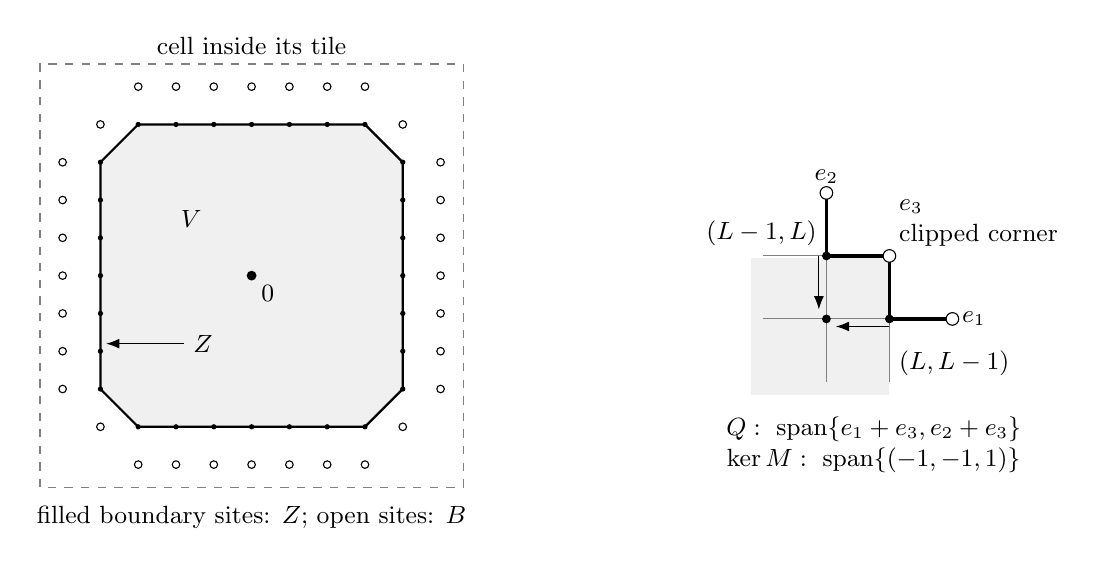
\begin{tikzpicture}[font=\small,>=Latex]
 \begin{scope}[x=0.48cm,y=0.48cm]
  \draw[dashed,gray] (-5.6,-5.6) rectangle (5.6,5.6);
  \fill[gray!12] (-4,-3)--(-3,-4)--(3,-4)--(4,-3)--
   (4,3)--(3,4)--(-3,4)--(-4,3)--cycle;
  \draw[thick] (-4,-3)--(-3,-4)--(3,-4)--(4,-3)--
   (4,3)--(3,4)--(-3,4)--(-4,3)--cycle;
  \foreach \j in {-3,-2,-1,0,1,2,3} {
   \foreach \sgn in {-1,1} {
    \fill (\sgn*4,\j) circle (0.07);
    \fill (\j,\sgn*4) circle (0.07);
    \draw[fill=white] (\sgn*5,\j) circle (0.1);
    \draw[fill=white] (\j,\sgn*5) circle (0.1);
   }
  }
  \foreach \sx in {-1,1} {
   \foreach \sy in {-1,1} {
    \draw[fill=white] (\sx*4,\sy*4) circle (0.1);
   }
  }
  \fill (0,0) circle (0.13) node[below right] {$0$};
  \node at (-1.6,1.5) {$V$};
  \node[above] at (0,5.6) {cell inside its tile};
  \draw[->] (-1.8,-1.8)--(-3.85,-1.8);
  \node[anchor=west] at (-1.8,-1.8) {$Z$};
  \node at (0,-6.4) {filled boundary sites: $Z$; open sites: $B$};
 \end{scope}
 \begin{scope}[shift={(8.1cm,0.25cm)},x=0.8cm,y=0.8cm]
  \fill[gray!12] (-2.2,-2.2) rectangle (0,-0.03);
  \draw[gray] (-2,-1)--(1,-1);
  \draw[gray] (-1,-2)--(-1,1);
  \draw[gray] (0,-2)--(0,0)--(-2,0);
  \draw[very thick] (0,-1)--(1,-1);
  \draw[very thick] (-1,0)--(-1,1);
  \draw[very thick] (0,-1)--(0,0)--(-1,0);
  \fill (0,-1) circle (0.07);
  \fill (-1,0) circle (0.07);
  \fill (-1,-1) circle (0.07);
  \draw[->] (0,-1.12)--(-0.85,-1.12);
  \draw[->] (-1.12,0)--(-1.12,-0.85);
  \draw[fill=white] (1,-1) circle (0.1) node[right] {$e_1$};
  \draw[fill=white] (-1,1) circle (0.1) node[above] {$e_2$};
  \draw[fill=white] (0,0) circle (0.1)
   node[above right,align=left] {$e_3$\\clipped corner};
  \node[below right] at (0,-1.35) {$(L,L-1)$};
  \node[above left] at (-1,0) {$(L-1,L)$};
  \node[align=center] at (-0.25,-3.0)
   {$Q:\ \operatorname{span}\{e_1+e_3,e_2+e_3\}$\\
    $\ker M:\ \operatorname{span}\{(-1,-1,1)\}$};
 \end{scope}
\end{tikzpicture}
\caption{The clipped cell and a magnified positive corner.  The two
boundary rows couple to a triple of exterior coordinates, leaving exactly
one missing direction.  The inward arrows reach a site outside $Z$;
this geometric fact is used in the transmission argument.}
\label{fig:clipped-cell}
\end{figure}

\subsection{Calibrating the root with a decaying profile}

We choose the root reference value so that the Dirichlet cell has a mode
at energy $E$. For arbitrary real values $v|_J$, write
\[
 A=\operatorname{Adj}_J+\diag_J(v-E).
\]
Whenever $A$ is invertible, define
\begin{equation}
 c(v)=E+p^\top A^{-1}p.
 \label{cell:calibrated-root}
\end{equation}
The Dirichlet matrix on $V$, with root potential $c(v)$, then satisfies
\begin{equation}
 \begin{pmatrix}c(v)-E&p^\top\\p&A\end{pmatrix}
 \begin{pmatrix}1\\-A^{-1}p\end{pmatrix}=0.
 \label{cell:dirichlet-mode}
\end{equation}
Thus invertibility of the punctured matrix $A$ permits resonance of the
full Dirichlet cell. We must choose the interior law so that $A^{-1}$ is
controlled, $c(v)$ stays inside the physical potential interval, and this
root-normalized mode is small at the boundary. The transmission estimates
will later control how it couples to an arbitrary passive exterior.

We first construct a comparison profile $\psi$, normalized by $\psi_0=1$,
and potentials $v^0$ satisfying its local equation. The profile is defined
also on $B$, where it is small but nonzero, so it need not be a Dirichlet
eigenvector. A deformation of this profile will give a polynomial inverse
bound for the punctured matrix at $v^0$. These two properties will control
the exact calibrated mode after the interior values are randomly perturbed.

Choose a rational multiple $\theta$ of $\pi$ and a real phase $\phi$ such
that
\begin{equation}
 |E-4\cos\theta|<h,
 \qquad m_\theta:=\min_{k\in\Z}|\cos(\theta k+\phi)|>0.
 \label{cell:carrier}
\end{equation}
The first choice is possible because the energy is in $(-4-h,4+h)$ and
rational multiples of $\pi$ are dense.  The sequence of cosine values is
periodic, so the second condition excludes only finitely many phases
modulo $2\pi$.  Put
\[
 d=\frac{h-|E-4\cos\theta|}{8}>0.
\]
Define the real sequence $f$ on all integers by
\begin{equation}
 \begin{aligned}
 f_0&=0,\\
 f_k+f_{k+1}
  &=\operatorname{sign}\bigl(\cos(\theta k+\phi)
                  \cos(\theta(k+1)+\phi)\bigr).
 \end{aligned}
 \label{cell:recurrence}
\end{equation}
Recursion in either direction gives $|f_k|\le|k|$.
For small fixed $\nu,c_u>0$, and $|u|\le c_u/L$, set
\begin{equation}
 \begin{aligned}
 \psi_x(u)&=e^{-\nu|x|_\infty}
       \frac{\cos(\theta(x_1+x_2)+\phi)}{\cos\phi}
       e^{u f_{x_1+x_2}}\quad(x\in V\cup B),\\
 v_x^0(u)&=E-\sum_{y\sim x}\frac{\psi_y(u)}{\psi_x(u)}
       \quad(x\in V).
 \end{aligned}
 \label{cell:profile-formula}
\end{equation}
Every neighbor in the last sum belongs to $V\cup B$ and $\psi_0=1$.
Uniformly over the allowed parameters,
\begin{equation}
 c e^{-\nu|x|_\infty}\le |\psi_x(u)|
       \le C e^{-\nu|x|_\infty}.
 \label{cell:profile-size}
\end{equation}
Indeed $|u f_{x_1+x_2}|$ is bounded by a fixed multiple of $c_u$ and the
periodic carrier is bounded away from zero.  For neighbors $x,y$ the
additional ratio factors differ from $1$ by $O(\nu+c_u)$: their radial
exponents differ by at most $\nu$, and
$|u(f_{y_1+y_2}-f_{x_1+x_2})|\le Cc_u$.  At $\nu=u=0$, the cosine
addition formula gives $v_x^0=E-4\cos\theta$.  We therefore fix $\nu,c_u$
small enough, once and for all, that
\begin{equation}
 |v_x^0(u)-(E-4\cos\theta)|\le d,
 \qquad |v_x^0(u)|\le h-7d.
 \label{cell:design-margin}
\end{equation}

\begin{lemma}[Choice of the profile parameter]\label{cell:profile}
There is a fixed exponent $C_2$ such that, for every sufficiently large
$L$, a deterministic $u_L\in[-c_u/L,c_u/L]$ can be chosen for which
the real symmetric Dirichlet matrix
\[
 A^0=\operatorname{Adj}_J+\diag_J(v^0-E)
\]
satisfies $\norm{(A^0)^{-1}}\le L^{C_2}$.  The bounds in
\Cref{cell:profile-size,cell:design-margin} hold for this
choice, with constants independent of $L$.
\end{lemma}

\begin{proof}
During the proof retain $u$ as a variable.  Let
$\Psi(u)=\diag(\psi_x(u):x\in J)$, $W(u)=\Psi(u)^2$, and
$Q(u)=-\Psi(u)A^0(u)\Psi(u)$.  Extend a test vector $\alpha$ by zero
at $0$ and on $B$.  Counting each unoriented edge meeting $J$ once gives
\begin{equation}
 \alpha^*Q(u)\alpha
 =\sum_{\{x,y\}:\{x,y\}\cap J\ne\varnothing}
       \psi_x(u)\psi_y(u)|\alpha_x-\alpha_y|^2.
 \label{cell:weighted-form}
\end{equation}
The sum here contains only edges with the other endpoint in $J\cup\{0\}
\cup B$.  Its weights may have either sign.  Nevertheless,
\Cref{cell:recurrence} gives the exact identity
\[
 \frac{\dd}{\dd u}\bigl(\psi_x(u)\psi_y(u)\bigr)
       =|\psi_x(u)\psi_y(u)|
       \quad(x\sim y).
\]
Thus $Q'(u)$ is a positive weighted Dirichlet form.

For each $x\in J$, choose a nearest-neighbor path to $0$ by decreasing
coordinates in absolute value.  It lies in $V$, has at most $2L$ edges,
and its max radius never exceeds $|x|_\infty$.  Every edge on the path
has weight $|\psi_y\psi_z|\ge c|\psi_x|^2$, by
\Cref{cell:profile-size}.  Weighted Cauchy--Schwarz along the path gives
\[
 |\psi_x|^2|\alpha_x|^2
 \le CL\sum_{\{y,z\}\text{ on the path}}
                  |\psi_y\psi_z||\alpha_y-\alpha_z|^2
 \le CL\,\alpha^*Q'(u)\alpha.
\]
Summing over at most $C L^2$ sites shows
\begin{equation}
 Q'(u)\ge cL^{-3}W(u)\ge L^{-C_1}W(u)
 \label{cell:form-monotonicity}
\end{equation}
for some fixed $C_1$, after increasing the lower size threshold.  One may
take $C_1=4$.  Moreover, all $W(u)$ in the allowed interval are comparable
as quadratic forms, with a fixed comparison constant, and
\[
 -CLW(u)\le W'(u)\le CLW(u).
\]

Choose $C_2>C_1+3$ and put $t=L^{-C_2}$.  For sufficiently large $L$,
\[
 (Q\pm tW)'\ge\tfrac12 L^{-C_1}W.
\]
More explicitly, form comparability and \Cref{cell:form-monotonicity}
give, whenever $u_2-u_1>C'tL^{C_1}$ with a sufficiently large fixed $C'$,
\begin{equation}
 Q(u_2)-tW(u_2)>Q(u_1)+tW(u_1).
 \label{cell:inertia-comparison}
\end{equation}
Let $\lambda_k(u)$ be the $k$th eigenvalue, in increasing order, of
$-A^0(u)$.  Congruence by the invertible real diagonal matrix $\Psi(u)$
preserves the numbers of negative, zero, and positive eigenvalues.
Consequently, if $\lambda_k(u_1)\ge-t$, the $k$th eigenvalue of
$Q(u_1)+tW(u_1)$ is nonnegative.  The strict inequality
in \Cref{cell:inertia-comparison} then makes the $k$th eigenvalue of
$Q(u_2)-tW(u_2)$ positive, so $\lambda_k(u_2)>t$.

It follows that each set
$\{u:|\lambda_k(u)|\le t\}$ has diameter at most $C'tL^{C_1}$.
No monotonicity assertion about the individual $\lambda_k(u)$ is needed.
The union of these sets, over $|J|=O(L^2)$ indices, has length at most
$C L^{C_1+2-C_2}=o(L^{-1})$, whereas the available interval has length
$2c_u/L$.  Choose $u_L$ outside this union.  For definiteness, one may
choose the first rational point in a fixed enumeration that belongs to
the open complement.  Then
$\dist(0,\operatorname{spec}A^0)>L^{-C_2}$, proving the inverse bound.
\end{proof}

From now on $u=u_L$ is fixed and suppressed in the notation.  Set
\begin{equation}
 \epsilon=e^{-\nu L},\qquad \sigma=\epsilon^2.
 \label{cell:epsilon}
\end{equation}
In particular, $|\psi_x|$ is comparable to $\epsilon$ on $B$ and on
$Z^+$, with constants independent of $L$. We have chosen the port strength
$\sigma$ as the square of this designed boundary-profile scale. The exact
calibrated mode will satisfy the polynomially lossy comparison in
\cref{cell:residual}.

\subsection{The branch sampler}

We first describe the boundary conditionings used by the sampler.  For
each corner triple use the fixed basis in \Cref{cell:corner-basis} and put
\begin{equation}
 \mathsf D_j=\diag\left(\frac{(r_j)_i}{n_i}:1\le i\le3\right)
 \quad(j=1,2).
 \label{cell:box-directions}
\end{equation}
These matrices satisfy
\[
 \mathsf D_jn=r_j,\qquad \tr\mathsf D_j=0,
 \qquad n^\top\mathsf D_jn=0.
\]
Thus a common shift changes the real diagonal in the missing direction
$n$, while a shift along $\mathsf D_j$ changes its coupling to $r_j$
without changing that diagonal. The three diagonal directions
$I,\mathsf D_1,\mathsf D_2$ are linearly independent:
multiplying a vanishing linear combination by $n$ gives a vanishing
linear combination of the orthonormal vectors $n,r_1,r_2$.
Thus centered coordinates $(s,t_1,t_2)$ specify physical potentials by
\begin{equation}
 \diag(v)=\diag(\bar v)+sI+t_1\mathsf D_1+t_2\mathsf D_2.
 \label{cell:box-coordinates}
\end{equation}
The map has a fixed nonzero Jacobian.  In fact its three columns, as
vectors of diagonal entries, are orthogonal and have length $\sqrt3$.
Use this same coordinate convention at all levels, including at exactly
coincident triples.

A prescribed corner box is the image under \Cref{cell:box-coordinates}
of a product of three centered intervals.  Fix an exponent $\kappa$.
The boxes allowed below have all three side lengths at least
$c(1+L)^{-\kappa}$ and at most $C$, lie at distance at least
$c(1+L)^{-\kappa}$ from the boundary of $(-h,h)^3$, and keep each physical
coordinate in a single polynomial piece of the fixed artificial profile
$\vartheta$.  Constants may depend on $\kappa$; in the hierarchy this
exponent is fixed by $K_0$.  Uniform measure in these box coordinates
is also uniform measure in the physical parallelepiped.  Because
$\vartheta$ is positive in the interior and comparable to squared
distance from the support endpoints, every nonzero artificial profile
$a_i\in\{1,\vartheta\}$ on a permitted box obeys
\begin{equation}
 a_i(v_i)\ge c(1+L)^{-2\kappa}.
 \label{cell:box-profile-lower}
\end{equation}
Increasing the exponent absorbs any fixed comparison constants.

Choose $D_1>C_2+2$.  A shell-depth parameter $D_2$ will be fixed after
the polynomial thresholds in the boundary and zero-jitter transmission
estimates have been fixed.  Finally choose $D_3$ sufficiently large
depending on $D_1,D_2$ and these thresholds.  On $J$ sample
\begin{equation}
 v_x=v_x^0+r\one_{Z^+}(x)+\zeta_x,
 \qquad r\sim\operatorname{Unif}[-L^{-D_1},L^{-D_1}],
 \label{cell:interior-sampler}
\end{equation}
where the $\zeta_x$ are independent centered uniforms of half-width
\begin{equation}
 w_x=
 \begin{cases}
 L^{-D_3},& L-|x|_\infty\le D_2\log L+5,\\
 \epsilon L^{-D_3},& L-|x|_\infty>D_2\log L+5.
 \end{cases}
 \label{cell:jitter-widths}
\end{equation}
They are independent of $r$ and all boundary sampling.

For these interior draws, use the matrix $A$ and the calibrated value
$c(v)$ from \cref{cell:calibrated-root}. At the root, put an open cell
port $a$ of strength $\sigma$, and use $c(v)$ as its real reference
potential. To define the hidden true potential, fix a smooth cutoff $\chi:\R\to[0,1]$ with $\chi=1$ on
$[-d,d]$ and $\supp\chi\subset[-2d,2d]$, and sample
\begin{equation}
 \begin{gathered}
 v_0=c(v)+\delta,\qquad
 \PP(\delta\in\dd t\mid v|_J)
   =\frac{1}{Z_\sigma}\chi(t)\frac{\sigma}{\pi(t^2+\sigma^2)}\,\dd t,\\
 Z_\sigma=\int_{\R}\chi(t)\frac{\sigma}{\pi(t^2+\sigma^2)}\,\dd t.
 \end{gathered}
 \label{cell:hidden-root}
\end{equation}
This is exactly the cutoff Cauchy law used in \Cref{mat:cutoff}.
The open reference $c(v)$ does not depend on the hidden draw $\delta$.

The boundary law is as follows.  On each corner triple sample uniformly
in its prescribed box, independently between the four triples.  On
every single side site $x$ sample
\begin{equation}
 v_x=\xi_x+s_0,\qquad
 \xi_x\sim\operatorname{Unif}[-h/4,h/4],\qquad
 s_0\sim\operatorname{Unif}[-h/4,h/4],
 \label{cell:side-law}
\end{equation}
using independent $\xi_x$ and one common $s_0$.  These draws are
independent of the triples and the interior draws.  Sites of the tile
outside $V\cup B$ retain their independent uniform $[-h,h]$ laws,
independently of all draws just described.  Apart from the common shifts
$r,s_0$ and the dependence of the root center $c(v)$ on $v|_J$, all
sampling is independent.

\begin{proposition}[Properties of the branch law]\label{cell:branch}
For sufficiently large $L$, the above choices have the following
properties, uniformly over permitted corner boxes:
\begin{enumerate}[label=(\roman*)]
 \item Every interior draw has
 \begin{equation}
  \norm{A^{-1}}\le2L^{C_2},\qquad
  \norm{-A^{-1}p-\psi|_J}\le C L^{C_2+1}\epsilon.
  \label{cell:residual}
 \end{equation}
 The exponents in these bounds are independent of $D_2$, provided $D_3$
 is subsequently chosen sufficiently large.
 \item All true potentials on $V$ lie in a fixed compact subinterval
 of $(-h,h)$.  The root center satisfies
 \begin{equation}
  |c(v)-v_0^0|\le C L^{C_2+1}\epsilon.
  \label{cell:root-calibration}
 \end{equation}
 The plateau of $\vartheta$ can therefore be fixed to contain every
 true value on $V$ and every single side value in $B$, for all the cells
 used.  The artificial absorptions on these sites are constant as
 $r$, the jitters, the common side shift, and the hidden root draw vary.
 \item Relative to the true product law on the tile conditioned on
 these same four corner boxes, the branch has a density
 $\mathcal L$ satisfying
 \begin{equation}
  0\le\mathcal L\le
       \exp\bigl(C L^3+C L^2\log L\bigr),
  \qquad \int\mathcal L\,\dd\PP_{\rm true,boxes}=1.
  \label{cell:likelihood}
 \end{equation}
 The corner-box conditional laws and the laws outside $V\cup B$ are
 unchanged.
\end{enumerate}
Artificial probes may have any prescribed mask of absent, constant, or
profile-dependent strengths, as in \Cref{mat:probes}.  For subsequent cell
estimates their common scale is restricted to
$0\le\tau\le e^{-c_*L}$, with a fixed $c_*>2\nu$.
\end{proposition}

\begin{proof}
The perturbation from $A^0$ is diagonal and has norm at most
$L^{-D_1}+L^{-D_3}$.  Taking $D_3>D_1$, \Cref{cell:profile} and a
Neumann series give the first bound in \Cref{cell:residual}.
The profile equation on $J$ gives the exact residual identity
\[
 A^0\psi|_J+p=-M\psi|_B.
\]
The right-hand side has norm at most $C\sqrt L\epsilon$.  On $Z^+$,
$|\psi_x|\le C\epsilon$, so the additional common-shift residual has
norm at most $CL\epsilon L^{-D_1}$.  On the jitter shell,
\[
 |\psi_x|\le C\epsilon L^{\nu D_2},
\]
where the extra depth $5$ has been absorbed in $C$.  Its jitter residual
is bounded by $CL\epsilon L^{\nu D_2-D_3}$.  Off that shell, the
half-width already has a factor $\epsilon$, and $|\psi_x|\le C$,
giving an upper bound $CL\epsilon L^{-D_3}$.
Thus $D_3>\nu D_2+2$ ensures
\[
 \norm{A\psi|_J+p}\le CL\epsilon.
\]
Multiplication by $A^{-1}$ proves the second bound in
\Cref{cell:residual}.  Notice that the resulting exponent $C_2+1$
was fixed before $D_2$.

Since $\psi_0=1$, the profile equation at $0$ reads
$v_0^0=E-p^\top\psi|_J$.  Subtracting this from the definition of $c(v)$
proves \Cref{cell:root-calibration}.  Increase the minimum cell size so
that all interior perturbations and the last calibration error are at
most $d$.  By \Cref{cell:design-margin}, $|v_x|\le h-6d$ on $J$,
$|c(v)|\le h-6d$, and $|v_0|\le h-4d$ after the hidden draw.
The side values lie in $[-h/2,h/2]$.  Choose the plateau to contain
these compact intervals.  This choice uses only the original design
margin $d$, and is therefore available before the large width and shell
exponents are fixed.  Each present artificial profile on these sites is
then identically $1$, proving the constancy assertion, also at the root.

For the density estimate, first condition on $r$ and $s_0$.  Each jitter
has density at most $(2w_x)^{-1}$ in its physical coordinate, hence
likelihood at most $h/w_x$ relative to a uniform $[-h,h]$ coordinate.
For small $\sigma$, $Z_\sigma\ge1/2$, so the conditional root density
is at most $C/\sigma$.  Its likelihood relative to the true uniform
coordinate is at most $C_h/\sigma$.  Each single side coordinate has
likelihood at most $4$.  Multiplying these bounds before averaging the
common shifts gives
\[
 \log\mathcal L
 \le C|J|+D_3|J|\log L+
       \nu L\,\#\{x\in J:w_x=\epsilon L^{-D_3}\}
       +2\nu L+C|B|
 \le C L^3+C L^2\log L.
\]
An upper bound of this form also holds when some individual displayed
logarithms are negative.  The four corner factors cancel against the
identical box conditionings in the reference law.  The outside factors
cancel as well.  All sampler laws are normalized, so integration gives
the last assertion in \Cref{cell:likelihood}.
\end{proof}

We record explicitly the order of choices used later.  The carrier,
$d,\nu,c_u,C_1,C_2$, the compact cutoff and plateau, and the corner-box
exponent are fixed first.  Next fix $D_1$.  The polynomial threshold in
\Cref{imp:weighted} and the regular inverse thresholds in the zero-jitter
part of \Cref{trans:cell} can then be fixed without $D_2,D_3$.
At depth $L-|x|_\infty=\lfloor D_2\log L\rfloor$,
\Cref{cell:profile-size} gives
\[
 \frac{|\psi_x|}{\epsilon}\ge cL^{\nu D_2}.
\]
Choose $D_2$ large enough that this dominates the already fixed
polynomial errors and reflected-field bounds in that argument.
Finally choose $D_3$ to satisfy both the residual requirements above and
the inverse and path-entry stability requirements of
\Cref{trans:cell}.  Enlarging $D_3$ changes neither the exponents in
\Cref{cell:residual} nor the earlier zero-jitter bounds.  All parameters
are now fixed; only after that do we increase the lower cell-size
threshold.  This order prevents the depth choice from depending on a
polynomial exponent that itself grows with the depth.

\section{A weighted projected impedance estimate}
\label{sec:impedance}

We retain the boundary geometry and the conditional boundary law of
\cref{cell:geometry,cell:branch}. In this section the interior of the cell
does not enter the calculation. Its only relevant feature is that it
couples to the boundary space through the projection $P$. We write
\[
 P=P_0+Q,
 \qquad Q=Q_1+Q_2+Q_3+Q_4,
\]
where $P_0$ projects onto the single side sites and $Q_a$ projects onto the
two-dimensional plane of the $a$th corner triple. The four complementary
directions in the triples are denoted by $n_a$. In the prescribed ordering
of each triple, $n_a=(-1,-1,1)/\sqrt3$. Thus $\rank Q=8$, whereas the
dimension of the whole boundary space is $O(L)$.

All norms below use the fixed real orthonormal bases of these spaces.
Constants may depend on the fixed disorder, profile, and corner-box
parameters. They will not depend on the exterior matrices, their norms,
the source vector, or the artificial-probe mask. Until an exponent $H$
is selected below, every expression denoted by $\operatorname{poly}(L)$
means a bound $C(1+L)^C$ whose constants are independent of $H$. A final
polynomial bound is allowed to depend on that selected, fixed exponent.

\begin{proposition}[Weighted projected impedance]
\label{imp:weighted}
Let $T$ be any fixed complex symmetric matrix on the boundary space with
$-\operatorname{Im}T\ge0$, and let $k$ be any fixed vector there. For each
boundary site prescribe $a_i$ to be one of $0$, $1$, and $\vartheta$, with
the prescription independent of the boundary variables. Set
\begin{equation}
 \mathcal T=T+\diag_B\bigl(v_i-i\tau a_i(v_i)\bigr),
 \qquad
 \rho=\norm{P(\mathcal T-iP)^{-1}k}^2.
 \label{imp:rho}
\end{equation}
Fix $c_*>0$ and suppose $0\le\tau\le e^{-c_*L}$. There are constants
$c>0$, $C<\infty$, and a sufficiently large lower threshold for $L$ such
that
\begin{equation}
 \E_B\!\left[
   \rho\,\one_{\{\norm{P\mathcal T^{-1}P}\le C(1+L)^C\}}
 \right]
 \ge c\,\E_B\rho.
 \label{imp:weighted-estimate}
\end{equation}
Here the expectation uses the boundary law conditional on its four
corner boxes. The constants are uniform in all the exterior data just
described. Moreover, changing only the single side variables to any other
bounded allowed settings, including their artificial absorptions,
changes $\rho$ by at most fixed multiplicative factors, pointwise wherever
the inverses exist.
\end{proposition}

The weight in \cref{imp:rho} matters: a small unweighted exceptional set
could contain nearly all the response of a weakly coupled exterior mode.
We first control the inverse on the corner planes $Q$ while leaving unit
absorption on the single side coordinates $P_0$. The corner estimates
must retain a fixed fraction of the response weight. We then average the
common real side shift to bound the whole projected inverse
$P\mathcal T^{-1}P$ with the auxiliary $P_0$ absorption removed.

\subsection{Elementary reductions and polynomial estimates}

We first record the comparison that permits bounded changes of the
absorbed coordinates.

\begin{lemma}[Comparison of absorbed responses]
\label{imp:comparison}
Suppose $D_1,D_2$ are invertible matrices with
$-\operatorname{Im}D_j\ge P$. If
$D_2-D_1=P\Delta P$ and $\norm{\Delta}\le K$, then, for every $k$,
\[
 (1+K)^{-1}\norm{PD_1^{-1}k}
 \le \norm{PD_2^{-1}k}
 \le (1+K)\norm{PD_1^{-1}k}.
\]
\end{lemma}

\begin{proof}
The inverse difference identity gives
\[
 PD_2^{-1}k
 =PD_1^{-1}k-PD_2^{-1}P\Delta PD_1^{-1}k.
\]
By \cref{mat:ward}, $\norm{PD_2^{-1}P}\le1$. This proves the upper
bound; interchanging the indices proves the lower bound.
\end{proof}

The inverses used in this section exist almost everywhere in the stated
boundary law. To see this without any nonsingularity assumption on $T$,
recall that a kernel vector of a passive matrix is annihilated by both its
Hermitian real and imaginary parts. Absorption on $P$ restricts such a
vector to the four missing directions. On that space the Hermitian real
part has the form of a fixed real symmetric matrix plus the independent
common corner shifts on its diagonal. Its determinant is a nonzero
polynomial, with the product of those shifts as its leading monomial.
The same reasoning applies after one missing direction is deleted or
after bounded changes in plane blocks. With absorption only on $P_0$,
a possible kernel lies on the full corner triples. The four common shifts
act there as scalar shifts on their respective three-dimensional blocks;
the determinant again has a nonzero leading monomial. Finally,
$\mathcal T$ itself has physical real diagonal variables with a joint
density, so its Hermitian real part is nonsingular
almost everywhere. These observations also justify almost-everywhere
slicing below.

The response weights are integrable. For example, writing
$G=(\mathcal T-iP)^{-1}$, the Ward identity implies
\[
 \norm{PGk}^2\le k^*(\operatorname{Im}G)k
 \le \norm{k}^2\tr\operatorname{Im}G.
\]
The joint law of the physical boundary diagonals has a bounded density on
a compact set; the bound here may depend on $L$. Slice that set along a
common real shift of all the physical diagonals. The phase estimate
\cref{mat:phase}, including its artificial-diagonal derivative term,
bounds the integral of $\tr\operatorname{Im}G$ along each slice. Integration
over the transverse coordinates proves finiteness. One may add
$-i\zeta\one$ first and pass to the limit by Fatou. In particular, after
some boundary variables are frozen, all integrals below are finite for
almost every such choice.

We shall use two elementary facts about polynomials. Their degree bounds
are fixed throughout this section.

\begin{lemma}[Polynomial norms and products]
\label{imp:polynomials}
On a rectangular box in a fixed number of real variables, let $p$ be a
polynomial of degree at most $d$ with values in a finite-dimensional
Hilbert space. There is a constant depending only on $d$ and the number
of variables such that
\begin{equation}
 \sup\norm{p}^2\le C\,\mathop{\mathrm{avg}}\norm{p}^2.
 \label{imp:poly-average}
\end{equation}
If the length of a coordinate interval is at least $\ell$, then
\begin{equation}
 \sup\norm{\partial_jp}\le C\ell^{-1}\sup\norm p.
 \label{imp:poly-derivative}
\end{equation}
If $q$ is a scalar polynomial of degree at most $d$, then
\begin{equation}
 \sup\norm{pq}\ge c\,\sup\norm p\,\sup\abs q.
 \label{imp:poly-product}
\end{equation}
The constants do not depend on the dimension of the target Hilbert space
or the side lengths of the box.
\end{lemma}

\begin{proof}
Affinely rescale the box to a unit cube. For scalar polynomials of bounded
degree, the asserted norm comparisons and derivative estimate follow
from equivalence of norms on a fixed finite-dimensional vector space.
For \cref{imp:poly-average}, choose a point where $\norm p$ is maximal
and a unit linear functional attaining that norm at that point; apply
the scalar estimate to its composition with $p$. The derivative estimate
follows in the same way by projecting at a maximizing derivative.

For the scalar product estimate, normalize the two supremum norms to
one. The two unit spheres of bounded-degree scalar polynomials are
compact. The supremum norm of their product has a positive minimum:
otherwise two nonzero limiting polynomials would have identically zero
product. Projecting the vector polynomial at one of its maximizing
points reduces \cref{imp:poly-product} to this scalar result.
\end{proof}

The following one-dimensional observation will prevent an extremely
narrow response peak from defeating a short-exception estimate.

\begin{lemma}[Resolution of a weighted slice]
\label{imp:resolution}
Let $I$ be an interval of length at least $\ell$, let $N$ be a
Hilbert-space-valued polynomial of fixed degree on $I$, and let $z$ be a
continuously differentiable complex function satisfying
\[
 \abs{z(s)}\ge c_0 a,
 \qquad \abs{z'(s)}\le C_0,
 \qquad a>0.
\]
Then
\[
 \sup_{s\in I}\frac{\norm{N(s)}^2}{\abs{z(s)}^2}
 \le \frac{C}{\min(\ell,a)}
       \int_I\frac{\norm{N(s)}^2}{\abs{z(s)}^2}\,\dd s.
\]
Here $C$ depends only on $c_0,C_0$ and the degree bound.
\end{lemma}

\begin{proof}
Take a maximizing point $s_0$ and an interval $I_0\subset I$ containing it,
of length a sufficiently small fixed multiple of $\min(\ell,a)$.
The derivative bound gives $\abs{z(s)}\le2\abs{z(s_0)}$ on $I_0$.
Applying \cref{imp:poly-average} on $I_0$ yields
\[
 \int_{I_0}\frac{\norm{N(s)}^2}{\abs{z(s)}^2}\,\dd s
 \ge \frac{c\abs{I_0}\norm{N(s_0)}^2}{\abs{z(s_0)}^2}.
\]
This proves the claim, including when $s_0$ is an endpoint.
\end{proof}

\subsection{Eight corner tests}

Remove the common shift from the single side variables and omit their
artificial absorptions. Denote the resulting boundary matrix by
$\mathcal T_0$, and set
\[
 w_0=\norm{P(\mathcal T_0-iP)^{-1}k}^2.
\]
The independent single side uniforms are still present. By
\cref{imp:comparison}, $w_0$ and $\rho$ are pointwise comparable by
fixed factors. We now hold those independent side uniforms fixed.

Choose an exponent $H$, to be fixed after the polynomial losses below,
and put
\[
 \eta=L^{-H},
 \qquad G_\eta=(\mathcal T_0-iP_0-i\eta Q)^{-1}.
\]
For each vector $b'$ in the eight prescribed real orthonormal corner-plane
bases, define
\begin{equation}
 \mathcal E_{b'}=
 \left\{\eta\operatorname{Im}(b'^\top G_\eta b')\ge\frac1{40}\right\}.
 \label{imp:test}
\end{equation}
Outside their union,
\begin{equation}
 \norm{Q(\mathcal T_0-iP_0)^{-1}Q}\le\eta^{-1}.
 \label{imp:Qgood}
\end{equation}
Indeed, if $\norm{QG_\eta Q}<(2\eta)^{-1}$, inverse difference and a
Neumann series give the bound in \cref{imp:Qgood}. Hence failure of that
bound forces $\norm{QG_\eta Q}\ge(2\eta)^{-1}$. Ward on $Q$ then gives
\[
 \eta\tr(Q\operatorname{Im}G_\eta Q)
 \ge \eta^2\norm{QG_\eta Q}_{\mathrm{HS}}^2\ge\frac14.
\]
If all eight tests fail to occur, the left side is less than $8/40<1/4$,
a contradiction.

Fix one test and condition on all boundary variables outside its corner
triple. Use centered box coordinates $(s,t_1,t_2)$ there, where $s$ is the
common shift and $t_j$ is the shift whose diagonal matrix maps the missing
direction $n$ to the plane basis vector $r_j$. In particular, the $t_j$
shift has zero $n,n$ entry. Write $t=(t_1,t_2)$. Every side length of the
box is at least $\ell\ge(1+L)^{-C}$ and at most a fixed constant. All
probabilities and averages on this box are normalized uniform ones.

There is first an unweighted bound
\begin{equation}
 \PP_{s,t}(\mathcal E_{b'})\le\operatorname{poly}(L)\eta.
 \label{imp:unweighted}
\end{equation}
For fixed $t$, apply \cref{mat:phase} while varying $s$. Its real
derivative is the identity on the tested triple. The artificial
derivatives satisfy the profile condition and are controlled by their
actual absorption, so the integral of the triple partial trace of
$\operatorname{Im}G_\eta$ is polynomially bounded. Since $b'$ is a unit
vector in that triple, its quadratic form is bounded by this trace.
Divide by the interval length, then average over $t$, to obtain
\cref{imp:unweighted}. Neither the phase range nor this polynomial loss
depends on $H$ or on the exterior norm.

We must strengthen \cref{imp:unweighted} to a bound for $w_0$-mass.

\subsection{A fixed remainder at one corner}

The exceptional test still uses the actual inverse $G_\eta$. To measure
its weight, we replace $w_0$ by a comparable response whose remainder
after deleting the tested missing direction $n$ is fixed. In
$\mathcal T_0-iP$, freeze the real variations of the tested triple
within its plane-plane block at the box center. Replace the artificial
absorption in that plane-plane block by $\tau$ times the plane identity.
Retain every fixed term from $T$ and retain all actual mixed terms and
the missing-direction diagonal. Call this modified matrix
$\widetilde D$.

The modification is bounded and supported on the tested plane. It also
preserves absorption at least $P$ plus the original artificial absorption
of the tested triple. In fact the change of artificial absorption is
\[
 \tau Q_a\bigl(\one-\diag(a_i(v_i))\bigr)Q_a\ge0,
\]
because $0\le a_i\le1$. Consequently
\begin{equation}
 C^{-1}w_0\le W:=\norm{P\widetilde D^{-1}k}^2\le Cw_0.
 \label{imp:modified-weight}
\end{equation}
The constant is fixed by \cref{imp:comparison}.

Delete the tested missing direction $n$, and denote the inverse of the
remaining block of $\widetilde D$ by $G_{\mathrm a}$. This inverse is
independent of $(s,t)$. The off-diagonal column from $n$ and its Schur
denominator have the form
\begin{align}
 p_1(s,t)&=p_{10}+t_1r_1+t_2r_2
       -i\tau\sum_{i\text{ in the triple}}a_i(v_i)n_iQe_i,
 \label{imp:p1}\\
 s-e(s,t)&=s-e_{\mathrm{fix}}
       -p_1^\top G_{\mathrm a}p_1
       -i\tau\sum_{i\text{ in the triple}}a_i(v_i)n_i^2.
 \label{imp:denominator}
\end{align}
The fixed vector $p_{10}$ may have components outside the tested triple;
no bound on it is assumed. All variable parts of $p_1$ lie in the tested
plane. The constants in \cref{imp:denominator} include the fixed diagonal
at $n$; there is no real $t$-dependent contribution to that diagonal.

Write $k_{\widehat n}$ for $k$ with its $n$ coordinate deleted, and set
\begin{equation}
 a=PG_{\mathrm a}k_{\widehat n},\qquad
 d_1=PG_{\mathrm a}p_1,\qquad
 \beta=p_1^\top G_{\mathrm a}k_{\widehat n}-k_n.
 \label{imp:adb}
\end{equation}
The block inverse formula yields
\begin{equation}
 W=\norm{a+\frac{d_1\beta}{s-e}}^2
   =\frac{\norm{N_1}^2}{\abs{s-e}^2},
 \qquad N_1=a(s-e)+d_1\beta.
 \label{imp:W}
\end{equation}
The norm of $d_1$ measures the response on the absorbed coordinates
induced by unit amplitude in the missing direction. The scalar Schur
denominator $s-e$ controls how sharply $W$ can concentrate. It need not agree with
the corresponding denominator in the actual test $G_\eta$.
Each profile lies on one fixed polynomial piece throughout the corner
box. Hence $p_1,d_1,\beta,e,N_1$ are polynomials in $(s,t)$ of bounded
degree, independently of all exterior data. Their coefficients need not
be bounded.

\begin{lemma}[Corner Schur estimates]
\label{imp:schur-estimates}
Uniformly throughout the box,
\begin{align}
 \operatorname{Im}e&\ge\norm{d_1}^2,
 &\abs{\partial_s e}&\le C\tau(1+\norm{d_1}),
 \label{imp:derivatives-a}\\
 \norm{\partial_s d_1}&\le C\tau,
 &\abs{\partial_s\beta}&\le C\tau\norm a,
 \label{imp:derivatives-b}\\
 \norm{\partial_{t_j}d_1}&\le C,
 &\abs{\partial_{t_j}e}&\le C(1+\norm{d_1}).
 \label{imp:derivatives-c}
\end{align}
If at least one artificial probe is present in the tested triple and
$\tau>0$, then also
\begin{equation}
 \operatorname{Im}e\ge\frac{\tau}{\operatorname{poly}(L)}.
 \label{imp:probe-floor}
\end{equation}
For every fixed $t$,
\begin{equation}
 \int\frac{\norm{d_1(s,t)}^2}{\abs{s-e(s,t)}^2}\,\dd s
 \le\int\operatorname{Im}\frac1{s-e(s,t)}\,\dd s
 \le\operatorname{poly}(L).
 \label{imp:s-integral}
\end{equation}
\end{lemma}

\begin{proof}
Apply absorption to the Schur extension
$(-G_{\mathrm a}p_1,1)$ at $n$. Its quadratic form under $\widetilde D$
is the scalar $s-e$, and its absorbed $P$-coordinates have norm
$\norm{d_1}$. This proves the first inequality. Every derivative of
$p_1$ is supported in the tested plane. Its $s$ derivative has size
$O(\tau)$, whereas its $t_j$ derivative is $r_j+O(\tau)$. Since
$\norm{PG_{\mathrm a}P}\le1$, these facts give the bounds on $d_1$.
Differentiating \cref{imp:denominator,imp:adb}, using transpose symmetry,
gives the other derivative bounds: for example,
\[
 \partial_s e
 =2(\partial_s p_1)^\top G_{\mathrm a}p_1
   +i\tau\sum_i\partial_s(a_i(v_i))n_i^2.
\]
The projection of $G_{\mathrm a}p_1$ onto the support of
$\partial_s p_1$ is controlled by $d_1$. Thus arbitrarily large fixed
components of $p_{10}$ cause no loss.

For \cref{imp:probe-floor}, an active profile in the triple is at least
an inverse polynomial, by the box clearance from the support endpoints.
If $\norm{d_1}\ge1/(2\sqrt3)$, the first bound already supplies a fixed
positive lower bound. Otherwise the corresponding physical coordinate
of $(-G_{\mathrm a}p_1,1)$ has modulus at least $1/(2\sqrt3)$, since
$\abs{n_i}=1/\sqrt3$. Its artificial absorption supplies
$\tau/\operatorname{poly}(L)$.

For the integral bound, let $y=\operatorname{Im}e$ and
$V=\operatorname{Im}(s-e)^{-1}=y/\abs{s-e}^2$. The first inequality
of \cref{imp:s-integral} follows from $y\ge\norm{d_1}^2$. If $e$ is
independent of $s$, ordinary scalar shift integration gives
$\int V\le\pi$; real poles are null sets. Otherwise $\tau>0$ and a
probe is present. Combining \cref{imp:derivatives-a,imp:probe-floor},
\[
 \frac{\abs{\partial_s e}}{\sqrt y}
 \le C\tau\left(\frac1{\sqrt y}+1\right)
 \le\operatorname{poly}(L).
\]
The argument of $s-e$ lies in $(-\pi,0)$, and its derivative is
\[
 \frac{\dd}{\dd s}\arg(s-e)
 =V-\operatorname{Im}\frac{\partial_s e}{s-e}.
\]
The error is bounded by $\operatorname{poly}(L)\sqrt V$. Young's
inequality absorbs half the integral of $V$; the remaining constant and
the phase variation are polynomially bounded on the bounded interval.
This proves \cref{imp:s-integral}.
\end{proof}

\subsection{Weighted exceptions when the coupling is appreciable}

Put
\[
 D=\max_{s,t}\norm{d_1(s,t)},\qquad \alpha_0=\frac1{100}.
\]
All maxima are taken over the closed box, which does not affect its
conditional law. The bound $\operatorname{Im}e\ge\norm{d_1}^2$ ties the
width of the response to this coupling. When $D\ge\eta^{\alpha_0}$, we
can isolate the few transverse parameters where the coupling becomes
small and use the unweighted test bound elsewhere. The case where $D$
is small throughout the box will instead require comparing the length
of each exceptional slice with its response width.

We first treat $D\ge\eta^{\alpha_0}$.

Suppose initially that $\abs{s-e}\ge1$ throughout the box. The maximum
and minimum of this denominator are then comparable by a fixed factor.
Indeed, \cref{imp:derivatives-b,imp:derivatives-c} show that $d_1$ varies
by at most a fixed constant. If $D$ is large, then
$\operatorname{Im}e\ge cD^2$ throughout, whereas the variation of
$s-e$ is at most $C(1+D)$. If $D$ is bounded, the same variation bound
and the assumed lower bound one suffice. By
\cref{imp:poly-average,imp:unweighted},
\begin{equation}
 \E_{s,t}[W\one_{\mathcal E_{b'}}]
 \le\operatorname{poly}(L)\eta\,\E_{s,t}W.
 \label{imp:comparable-case}
\end{equation}

It remains to consider the case where $\abs{s-e}<1$ somewhere. At that
point $\norm{d_1}<1$; the derivative bounds then imply that $D$ is
bounded throughout the box. Since $s$ is bounded, the same argument
shows that $e$ and $s-e$ are bounded as well. Set
\[
 M_1=\max\norm{N_1},\qquad B_1=\max\abs\beta.
\]
The bounded denominator and \cref{imp:poly-average} give
\begin{equation}
 \E_{s,t}W\ge cM_1^2.
 \label{imp:weight-lower}
\end{equation}
Furthermore,
\begin{equation}
 \norm a+DB_1\le\operatorname{poly}(L)M_1.
 \label{imp:numerator-control}
\end{equation}
Here is the required quantitative argument. By the product estimate,
\[
 DB_1\le C\max\norm{d_1\beta}
       \le C(M_1+\norm a).
\]
Differentiate $N_1=a(s-e)+d_1\beta$ in $s$ and use
\cref{imp:poly-derivative,imp:derivatives-a,imp:derivatives-b}. As $D$
is bounded, this gives
\[
 \norm a\le C\ell^{-1}M_1+C\tau(\norm a+B_1).
\]
Substitute the preceding estimate for $B_1$. Since
$D\ge\eta^{\alpha_0}$, the coefficient
$C\tau(1+D^{-1})$ is less than one half for sufficiently large $L$
after $H$ is fixed. Absorption proves \cref{imp:numerator-control}.
Its polynomial exponent is independent of $H$.

Choose $\Delta=\eta^{1/8}$ and let
\[
 \mathcal A=\{t:\min_s\norm{d_1(s,t)}<\Delta\}.
\]
Then
\begin{equation}
 \PP_t(\mathcal A)\le C\frac{\Delta}{D}.
 \label{imp:affine-sublevel}
\end{equation}
To prove this, \cref{imp:p1} and Ward show that $d_1(s,t)$ is within
$C\tau$ of an affine function of $t$, uniformly in $s$. Rescale the two
$t$ intervals to unit intervals. If $\mathcal A$ is nonempty, the affine
function has a value of norm at most $\Delta+C\tau$, and its maximum
norm is at least $D-C\tau$. Project it by a real unit linear functional
attaining that latter norm. Because $\Delta/D\to0$ and $\tau\ll\Delta$,
one of the two scalar slopes has magnitude at least $cD$. Slicing in
that coordinate bounds the fraction where the scalar magnitude is at
most $\Delta+C\tau$ by $C\Delta/D$. This includes $\mathcal A$.

For each $t\in\mathcal A$, \cref{imp:W,imp:s-integral} gives
\[
 \E_s W\le\operatorname{poly}(L)(\norm a^2+B_1^2)
 \le\operatorname{poly}(L)(1+D^{-2})M_1^2.
\]
On the complement of $\mathcal A$, absorption gives
$\abs{s-e}\ge\norm{d_1}^2\ge\Delta^2$, so
$W\le\Delta^{-4}M_1^2$. Using \cref{imp:unweighted} there and
\cref{imp:affine-sublevel} on $\mathcal A$, we obtain
\begin{equation}
 \E_{s,t}[W\one_{\mathcal E_{b'}}]
 \le\operatorname{poly}(L)
     \left(\frac{\Delta}{D^3}+\frac{\eta}{\Delta^4}\right)
     \E_{s,t}W.
 \label{imp:first-case}
\end{equation}
We used the boundedness of $D$ and \cref{imp:weight-lower} in the last
step. If $M_1=0$, all the weighted integrals vanish and the inequality
holds directly. In particular, this argument never divides by a possibly
zero expected weight. The powers in \cref{imp:first-case} satisfy
\[
 \frac{\Delta}{D^3}\le\eta^{1/8-3\alpha_0},
 \qquad \frac\eta{\Delta^4}=\eta^{1/2},
 \qquad \frac18-3\alpha_0>0.
\]

\subsection{Weighted exceptions when the coupling is small}

We now assume $D<\eta^{\alpha_0}$ and write $b'=r_j$ for the tested
basis vector. Vary $t_j$ between two points separated by at least half
its interval length. From \cref{imp:p1,imp:adb},
\begin{equation}
 a_{b'}:=PG_{\mathrm a}b',
 \qquad
 \norm{a_{b'}}\le C\ell^{-1}(D+\tau).
 \label{imp:small-b}
\end{equation}
This can be made as small as a prescribed fixed constant by choosing
$H$ sufficiently large, then $L$ sufficiently large. The inference uses
variation over the whole $t_j$ interval; it does not assume that the
exterior has a lower bound on its coupling.

Next delete $n$ in the actual matrix $G_\eta^{-1}$, without freezing its
plane block. Let $G_{\eta,\mathrm{rem}}$ denote the remaining inverse,
put
\[
 d_{1,\eta}=PG_{\eta,\mathrm{rem}}p_1,
\]
and write $s-e_\eta$ for its Schur denominator at $n$. Its off-diagonal
column is exactly the same $p_1$ as before. The remaining matrices for
$G_{\mathrm a}$ and $G_{\eta,\mathrm{rem}}$ differ by a bounded matrix
supported on $Q$. Moreover,
$\norm{QG_{\eta,\mathrm{rem}}Q}\le\eta^{-1}$ by Ward. Inverse
difference and symmetry therefore give
\begin{align}
 \eta\abs{b'^\top G_{\eta,\mathrm{rem}}b'}
   &\le C\norm{a_{b'}},
 \label{imp:small-comparison-a}\\
 \abs{b'^\top d_{1,\eta}}
   &\le\abs{b'^\top d_1}
       +C\norm{a_{b'}}\norm{Qd_{1,\eta}}.
 \label{imp:small-comparison-b}
\end{align}
For clarity, the inverse identity used in both estimates is
$G_{\eta,\mathrm{rem}}
=G_{\mathrm a}+G_{\mathrm a}\Delta G_{\eta,\mathrm{rem}}$,
where $\Delta=Q\Delta Q$ has bounded norm. The first left factor is thus
controlled by $PG_{\mathrm a}b'$, regardless of the exterior norm.

Take the bound in \cref{imp:small-b} small enough that the first term
in the Schur inverse formula cannot by itself cause
$\mathcal E_{b'}$. On that exception,
\begin{equation}
 \frac{\eta\abs{b'^\top d_{1,\eta}}^2}{\abs{s-e_\eta}}
 \ge c.
 \label{imp:exception-schur}
\end{equation}
On the other hand, absorption on the actual Schur extension yields
\[
 \operatorname{Im}e_\eta\ge\eta\norm{Qd_{1,\eta}}^2.
\]
Together with \cref{imp:exception-schur}, this implies
$\norm{Qd_{1,\eta}}\le C\abs{b'^\top d_{1,\eta}}$. Insert
\cref{imp:small-comparison-b} and absorb its small last coefficient.
We conclude that, on the exception,
\begin{equation}
 \norm{Qd_{1,\eta}}\le C\norm{d_1},
 \qquad
 \abs{s-e_\eta}\le C\eta\norm{d_1}^2.
 \label{imp:small-exception}
\end{equation}

The exceptional set is short on every almost-everywhere $s$ slice.
To establish this rigorously, let
$D_t=\max_s\norm{d_1(s,t)}$. Differentiating the actual Schur formula
shows that, on the exception,
\[
 \abs{\partial_s e_\eta}
 \le C\norm{Qd_{1,\eta}}^2
       +C\tau(1+\norm{Qd_{1,\eta}})
 \le C D^2+C\tau(1+D)<\frac12.
\]
The first term comes from the real derivative of the tested plane
block. Its artificial derivative is absorbed in the same bound; the
mixed and missing-direction derivatives give the terms containing
$\tau$. Thus $\operatorname{Re}(s-e_\eta)$ has derivative at least
one half on the exception.

There are only boundedly many components of that exceptional slice away
from poles. Indeed, with all other variables fixed, the matrix varies
polynomially only on the three coordinates of the tested triple.
In a basis containing those coordinates, expansion of the determinant
uses variable factors from at most three rows. Its degree, and the
degrees of the relevant cofactors, are bounded by a constant depending
only on the profile degree, not on the dimension or norm of the exterior.
The same assertion holds after deleting $n$. Clearing the squared
absolute value of a denominator converts \cref{imp:test} into a real
polynomial inequality of bounded degree. Such a set has a bounded
number of intervals and isolated points, except for poles, which also
have bounded number on an almost-everywhere slice.

On each interval component, \cref{imp:small-exception} confines
$\operatorname{Re}(s-e_\eta)$ to an interval of length
$C\eta D_t^2$, while its derivative is at least one half. Summing over
the bounded number of components gives
\begin{equation}
 \abs{\{s:(s,t)\in\mathcal E_{b'}\}}
 \le C\eta D_t^2.
 \label{imp:slice-length}
\end{equation}
If $D_t=0$, \cref{imp:small-exception} and the Schur formula rule out
the exception off its null set of poles.

For $D_t>0$, the denominator of the modified weight has a matching
minimum scale:
\begin{equation}
 \operatorname{Im}e(s,t)\ge cD_t^2
 \quad\hbox{throughout the slice},
 \qquad
 \abs{\partial_s(s-e)}\le C.
 \label{imp:linewidth}
\end{equation}
Here is the point requiring the artificial-absorption floor. By
\cref{imp:derivatives-b}, the oscillation of $d_1$ on the slice is
$O(\tau)$. If its norm is everywhere at least $D_t/2$, absorption proves
the first bound immediately. Otherwise $D_t\le C\tau$. In this latter
case an artificial term must be present, since without one $d_1$ is
independent of $s$. Now \cref{imp:probe-floor} gives
$\operatorname{Im}e\ge\tau/\operatorname{poly}(L)\ge cD_t^2$
for sufficiently large $L$. The derivative bound follows from
\cref{imp:derivatives-a} and $D<\eta^{\alpha_0}$.

The exceptional length $O(\eta D_t^2)$ must be compared with the
resolution $\min(\ell,D_t^2)$ supplied by the modified denominator.
The real parts of the two Schur denominators need not vanish at the same
point. Apply \cref{imp:resolution} to $N_1$ and $s-e$, using
\cref{imp:linewidth}. It gives
\[
 \max_s W(s,t)
 \le\frac{C}{\min(\ell,D_t^2)}\int W(s,t)\,\dd s.
\]
Combining with \cref{imp:slice-length},
\[
 \int W(s,t)\one_{\mathcal E_{b'}}\,\dd s
 \le\frac{C\eta D_t^2}{\min(\ell,D_t^2)}
       \int W(s,t)\,\dd s
 \le\operatorname{poly}(L)\eta\int W(s,t)\,\dd s.
\]
The last inequality uses $D_t\le D<1$ and the inverse-polynomial lower
bound on $\ell$. Averaging over $t$ proves
\begin{equation}
 \E_{s,t}[W\one_{\mathcal E_{b'}}]
 \le\operatorname{poly}(L)\eta\,\E_{s,t}W
 \label{imp:second-case}
\end{equation}
in the small-coupling case. This estimate remains uniform as the coupling
vanishes; no positive lower bound for $D$ was used here.

\subsection{Restoring the side shift}

We now choose the parameters. All polynomial losses in
\cref{imp:comparable-case,imp:first-case,imp:second-case}, and the box
width exponent, have been fixed independently of $H$. Choose $H$ large
enough that their products with
\[
 \eta^{1/8-3\alpha_0},\qquad \eta^{1/2},\qquad\eta
\]
tend to zero, and that \cref{imp:small-b} is uniformly small in its
case. With this $H$ fixed, take $L$ sufficiently large that
$\tau\ll\Delta$, $\tau/\eta^{\alpha_0}\ll1$, and all preceding
absorptions are valid. The assumption $\tau\le e^{-c_*L}$ ensures every
one of these requirements for any fixed $c_*>0$.

For each of the eight tests, condition on the other corner variables,
apply the appropriate estimate, and compare $W$ with the same weight
$w_0$ by \cref{imp:modified-weight}. Integration and summation give
\begin{equation}
 \E[w_0\one_{\mathcal G}]\ge\frac34\E w_0,
 \qquad
 \mathcal G=\bigcap_{b'}\mathcal E_{b'}^c,
 \label{imp:weighted-Qgood}
\end{equation}
for sufficiently large $L$. This is still conditional on the independent
side uniforms. The threshold can be chosen uniformly in those frozen
values and in all exterior data. Zero conditional weights cause no
difficulty, since every estimate was an inequality between integrals.

Fix data in $\mathcal G$, before restoring the common side shift. On the
space $P$ consider the rational matrix function
\[
 F(z)=P(\mathcal T_0+zP_0)^{-1}P,
 \qquad\operatorname{Im}z<0.
\]
It is analytic there and has nonnegative imaginary part. To check
analyticity, a kernel at one point of the lower half-plane would be
annihilated by $P_0$ and by $\mathcal T_0$, hence would also be a kernel
at $z=-i$, where the inverse exists. On $\mathcal G$,
\cref{imp:Qgood} bounds the $Q,Q$ block of $F(-i)$ by $\eta^{-1}$.
Ward gives a bound one on the $P_0,P_0$ block and
\[
 \norm{P_0(\mathcal T_0-iP_0)^{-1}Q}^2
 \le\norm{Q\operatorname{Im}(\mathcal T_0-iP_0)^{-1}Q}
 \le\eta^{-1}.
\]
Transpose symmetry gives the same bound on the other mixed block. Thus
\begin{equation}
 \norm{F(-i)}\le C\eta^{-1}.
 \label{imp:center-bound}
\end{equation}

For completeness, map the unit disk to the lower half-plane by
$z=-i(1+w)/(1-w)$. Then $-iF(z(w))$ has positive semidefinite Hermitian
real part, and its value at zero obeys \cref{imp:center-bound}. The
positive-real-part weak estimate \cref{mat:positive-real-extension} gives
a boundary weak-$L^1$ bound at most
$C(\rank P)\eta^{-1}$. One can obtain this bound directly from the
positive matrix measure in its Herglotz representation: its total trace
mass is at most $(\rank P)\norm{F(-i)}$, while the constant imaginary
part has the same polynomial bound. The boundary change of variable
sends Haar measure to $\dd x/(\pi(1+x^2))$.

The Cauchy density has a positive lower bound on the fixed interval
$[-h/4,h/4]$. Therefore there is a polynomial
$R_L=C(1+L)^C$, now allowed to depend on $H$, such that for at least
half the common side shifts $x$ in their prescribed uniform law,
\begin{equation}
 \norm{P(\mathcal T_0+xP_0)^{-1}P}\le R_L.
 \label{imp:side-good}
\end{equation}
This conclusion uses only the norm at $-i$, not the norm of $T$.

Restore the artificial absorptions at the single side sites. Their
change has norm at most $\tau$ and is supported on $P_0$. For a shift
satisfying \cref{imp:side-good}, the inverse difference identity on $P$
and a Neumann series give
\[
 \norm{P\mathcal T^{-1}P}\le2R_L
\]
as soon as $\tau R_L\le1/2$. This holds for sufficiently large $L$.
Throughout the common-shift average, with or without these side
absorptions, \cref{imp:comparison} compares the weight to $w_0$ by
fixed factors. Hence at least a fixed fraction of the $\rho$-weight
survives the good shifts for every corner setting in $\mathcal G$.
Integrate this statement, use \cref{imp:weighted-Qgood}, and finally
average over the initially frozen independent side uniforms. Since
$\E\rho$ and $\E w_0$ are comparable, this proves
\cref{imp:weighted-estimate}. The pointwise comparison assertion in
\cref{imp:weighted} is already contained in \cref{imp:comparison}.
\hfill$\square$

\subsection{The Schur form used by the interior}

The following formulation makes the interface with the transmission
calculation explicit.

\begin{corollary}[Eliminating the missing directions]
\label{imp:schur-interface}
Let $N=\one-P$ on the boundary space. Almost everywhere in the boundary
law, the $N,N$ block of $\mathcal T$ is invertible. Define its Schur
matrix and transformed source by
\begin{align*}
 \widehat T
 &=P\mathcal TP-P\mathcal TN(N\mathcal TN)^{-1}N\mathcal TP,\\
 \widehat k
 &=Pk-P\mathcal TN(N\mathcal TN)^{-1}Nk.
\end{align*}
Then $\widehat T$ is complex symmetric and passive, and
\begin{align*}
 \widehat T^{-1}&=P\mathcal T^{-1}P,\\
 \widehat k&=\widehat T P\mathcal T^{-1}k,\\
 P(\mathcal T-iP)^{-1}k&=(\widehat T-i\one_P)^{-1}\widehat k.
\end{align*}
In particular $\rho=\norm{(\widehat T-i\one_P)^{-1}\widehat k}^2$,
and \cref{imp:weighted-estimate} controls $\widehat T^{-1}$ on a set
carrying a fixed fraction of this weight.
\end{corollary}

\begin{proof}
On the four-dimensional space $N$, the Hermitian real part is a fixed
real symmetric matrix plus the four common corner shifts on its
diagonal; the traceless box directions have zero diagonal entry there.
Its determinant is a nonzero polynomial, so the block is invertible
almost everywhere by passivity and the density of those shifts. The
identities are the block inverse and source elimination formulas.
Symmetry and passivity persist under Schur elimination by
\cref{mat:ward}.
\end{proof}

\section{Transmission through a cell}
\label{sec:transmission}

Throughout this section, the geometry and branch parameters are those of
\Cref{cell:geometry,cell:profile,cell:branch}. Constants may depend on the
fixed energy, disorder, profile, corner-box exponents, and parameters
already chosen, but not on exterior matrices or source vectors. A
polynomial bound means $C(1+L)^C$ with this convention; different occurrences
may have different exponents. All assertions concern sufficiently large
$L$ after the parameters have been fixed.

\subsection{Exterior data and the two branch estimates}

Suppose that the root is the only cell port in $V\cup B$, and that the
source port lies outside this set. Artificial probes with a prescribed
mask may be present. Eliminate the exterior physical sites. Its effect
on $B$ is a fixed complex-symmetric passive matrix $T$, and the source
gives a fixed vector $k$, including its input multiplier. The remaining
boundary matrix is
\[
 \mathcal T=T+\diag_B\bigl(v_i-i\tau a_i(v_i)\bigr).
\]
The exterior is held fixed throughout the cell integration, as are the
four corner boxes. In particular, no bound on $\norm{T}$ or $\norm{k}$ is
assumed.

Let $P$ also denote its range, equipped with a real orthonormal basis.
Eliminating the four missing boundary directions gives
\begin{equation}
 \widehat T=(P\mathcal T^{-1}P)^{-1},\qquad
 \widehat k=\widehat T P\mathcal T^{-1}k,\qquad
 k_*=(\widehat T-iI_P)^{-1}\widehat k,\qquad
 \rho=\norm{k_*}^2.
 \label{trans:normalization}
\end{equation}
These formulas are used at their almost-everywhere inverses. The
missing-direction block is generically invertible by
\Cref{imp:schur-interface}. Schur complementation
preserves symmetry and passivity, and gives the identity
\[
 k_*=P(\mathcal T-iP)^{-1}k.
\]
Thus $\rho$ is exactly the weight in \Cref{imp:weighted}, and
\begin{equation}
 \norm{(\widehat T-iI_P)^{-1}}\le1.
 \label{trans:absorbed-exterior}
\end{equation}
Hereafter $M$ is restricted to $P$, and is extended by a zero row at the
root when it is regarded as a map into $V$.

Let $G$ be the inverse on $V\oplus P$ with the root open, reference
potential $c(v)$, and root strength $\sigma=\epsilon^2$. Its internal
artificial absorptions are constant during the branch integration:
the true values lie on the plateau specified in \Cref{cell:branch}.
Set
\begin{equation}
 u=\sqrt\sigma\,Ge_0,\qquad g=\sigma G_{00},\qquad
 t=\widehat k^\top u_P.
 \label{trans:amplitude}
\end{equation}
Since $k$ includes the source input multiplier, the root-to-source
scattering amplitude satisfies $\abs{S_{\mathrm{source},a}}^2=4\abs t^2$.
The sign convention for the source does not affect this identity.
The inverse exists almost everywhere even though $c(v)$ depends on
other potentials. Indeed,
absorption forces a kernel vector to vanish at the root. Restoring its
true real diagonal therefore preserves that vector. After eliminating
the fixed boundary data, the real part is a fixed matrix plus the true
real diagonals on $V$; their absolutely continuous joint law makes its
determinant nonzero almost everywhere. This also justifies the
almost-everywhere slices used below.

\begin{proposition}[Branch transmission]\label{trans:cell}
Choose the branch parameters in the order described below and fix
$c_*>2\nu$. For $0\le\tau\le e^{-c_*L}$, uniformly in the fixed exterior
data and allowed corner boxes,
\begin{align}
 \E\abs{t}^2
 &\ge e^{-C(\log L)^2}\,\E_B\rho,
 \label{trans:lower}\\
 \E\bigl[\abs\mu\,\abs{t}^2\bigr]
 &\le e^{-cL}\,\E\abs{t}^2.
 \label{trans:relative}
\end{align}
Here $\mu$ is the conditional single-root closure coefficient of
\Cref{mat:closure,mat:cutoff}. The expectation is the branch expectation,
and $\E_B$ averages its boundary law. The hidden root value has already
been averaged in $\mu$; averaging it again does not change any other
quantity in these formulas.
\end{proposition}

\subsection{The cutoff error and the small-response region}

We first derive \Cref{trans:relative} assuming \Cref{trans:lower}.
Fix the boundary data and all jitters, and vary the common real shift
$r$ on $Z^+$. Write $P_+$ for the coordinate projection onto $Z^+$,
extended by zero on the root and on $P$. Since
$c(v)=E+p^\top A^{-1}p$ and $A'=P_+$ on $J$, differentiation gives
\begin{equation}
 c'=-\norm{P_+A^{-1}p}^2,\qquad
 g'=-u^\top P_+u-\sigma^{-1}c'g^2.
 \label{trans:shift-derivatives}
\end{equation}
The profile estimate in \Cref{cell:residual}, together with
$\abs{\psi_i}\le C\epsilon$ on $Z^+$, implies
$\abs{c'}/\sigma\le C(1+L)^C$. Root absorption and
\Cref{mat:ward} imply
\begin{equation}
 \abs g^2\le\operatorname{Im}g\le1.
 \label{trans:g-ward}
\end{equation}

Let $I_r=[-L^{-D_1},L^{-D_1}]$. The derivative of a continuous
determinant phase of $G^{-1}$ is
\[
 \Phi'(r)=\tr(P_+\operatorname{Im}G P_+)
       +\frac{c'}{\sigma}\operatorname{Im}g.
\]
The phase has range at most $\pi\dim(V\oplus P)$ after strict
regularization. Integrating, using \Cref{trans:g-ward}, and then
removing the regularization as in \Cref{mat:phase} gives
\begin{equation}
 \int_{I_r}\tr(P_+\operatorname{Im}G P_+)\,\dd r
 \le C(1+L)^C.
 \label{trans:phase-trace}
\end{equation}
In particular, Ward and symmetry bound the integral of
$\norm{P_+u}^2$ by the same polynomial. We need an additional factor
when $g$ is small.

Put $D=-\operatorname{Im}G^{-1}$. Complex symmetry makes $D$ real
symmetric and gives
\[
 u-\overline u=2iG^*Du,\qquad
 u^*Du=\operatorname{Im}g.
\]
For each coordinate, Cauchy--Schwarz in the form $D$ bounds the square
of the corresponding entry of $G^*Du$ by
$(\operatorname{Im}G)_{ii}\operatorname{Im}g$. Consequently, with
entrywise imaginary part on vectors,
\begin{equation}
 \norm{P_+\operatorname{Im}u}^2
 \le (\operatorname{Im}g)
       \tr(P_+\operatorname{Im}G P_+).
 \label{trans:imaginary-vector}
\end{equation}
Take $q=\sqrt\sigma=\epsilon$, and set
$\Omega_q=\{r\in I_r:\abs{g(r)}\le q\}$, excluding null singular
sets. \Cref{trans:phase-trace,trans:imaginary-vector} give
\[
 \int_{\Omega_q}\norm{P_+\operatorname{Im}u}^2\,\dd r
 \le C(1+L)^Cq.
\]

There are only polynomially many component intervals of $\Omega_q$.
To see this, $A$ is affine in $r$, $c$ is a rational function obtained
by inverting $A$, and $G$ is a further matrix inverse in cell dimension
$O(L^2)$. Thus numerator and denominator degrees of $g$ are bounded
by a fixed polynomial in $L$. The inequality $\abs g^2\le q^2$
becomes a real polynomial inequality after clearing the squared
denominator. Its intervals and the poles are therefore polynomially
many; the values of the exterior coefficients do not affect this
degree bound. Integrate the real part of
\Cref{trans:shift-derivatives} on these intervals, first truncating
away from any endpoints where necessary. Every endpoint value of
$\operatorname{Re}g$ has modulus at most $q$. Hence
\[
 \int_{\Omega_q}\operatorname{Re}(u^\top P_+u)\,\dd r
 \le C(1+L)^Cq+C(1+L)^Cq^2\abs{I_r}.
\]
Using
$\norm{P_+u}^2=\operatorname{Re}(u^\top P_+u)
 +2\norm{P_+\operatorname{Im}u}^2$, we obtain
\begin{equation}
 \int_{\Omega_q}\norm{P_+u}^2\,\dd r
 \le C(1+L)^Cq.
 \label{trans:small-response}
\end{equation}
Normalized uniform integration in $r$ only introduces the polynomial
factor $(2L^{-D_1})^{-1}$.

The $Z$ rows of the equation $G^{-1}u=\sqrt\sigma e_0$ involve only
$u_P$ and $P_+u$. Their coefficients are uniformly bounded, and $M$
is bounded below on $P$. The $P$ rows then give, respectively,
\[
 \norm{u_P}\le C\norm{P_+u},\qquad
 \widehat T u_P=-M^\top u_J,\qquad
 \norm{\widehat T u_P}\le C\norm{P_+u}.
\]
It follows from symmetry and \Cref{trans:normalization} that
\begin{equation}
 \abs t
 =\abs{k_*^\top(\widehat T-iI_P)u_P}
 \le C\sqrt\rho\,\norm{P_+u}.
 \label{trans:source-control}
\end{equation}
The cutoff bounds in \Cref{mat:cutoff} now yield
\begin{equation}
 \E\bigl[\abs\mu\,\abs t^2\bigr]
 \le Cq\E\abs t^2+C(1+L)^Cq\E_B\rho.
 \label{trans:relative-prelower}
\end{equation}
The first term treats $\abs g>q$; the second follows from
\Cref{trans:small-response,trans:source-control} on $\Omega_q$.
Since $q=e^{-\nu L}$, substitution of \Cref{trans:lower} absorbs
the factor $e^{C(\log L)^2}$ and proves \Cref{trans:relative} for
some fixed $c>0$.

\subsection{Regular boundary and shift data}

We turn to \Cref{trans:lower}. By \Cref{imp:weighted}, it is enough
to work on boundary data satisfying
\begin{equation}
 \norm{\widehat T^{-1}}\le C(1+L)^C,
 \label{trans:good-boundary}
\end{equation}
since this event carries a fixed positive fraction of $\E_B\rho$.
Fix such data, assume $\rho>0$, and initially set every jitter to zero.
Define the boundary Schur matrix
\[
 \mathcal B=\widehat T-M^\top A^{-1}M.
\]
We claim that at least half of the uniform $r$-interval satisfies
\begin{equation}
 \norm{\mathcal B^{-1}}\le C(1+L)^C.
 \label{trans:regular-r}
\end{equation}
All exponents in this assertion can be fixed before $D_2,D_3$.

Indeed,
\[
 \mathcal B'=M^\top A^{-1}P_+A^{-1}M\ge cI_P.
\]
For the last inequality, put $w=A^{-1}Mx$. The $Z$ rows of $Aw=Mx$
have bounded coefficients, use only $P_+w$, and give
$\norm{Mx}\le C\norm{P_+w}$. The lower singular-value bound for
$M$ gives $\norm{P_+w}\ge c\norm x$, which proves the assertion.
For $\xi>0$ let $K_\xi=(\mathcal B-i\xi I_P)^{-1}$. If
$\norm{\mathcal B^{-1}}>\xi^{-1}$, inverse difference implies
$\norm{K_\xi}\ge(2\xi)^{-1}$. Ward then implies
\begin{equation}
 \xi\tr\operatorname{Im}K_\xi\ge\frac14.
 \label{trans:regular-test}
\end{equation}
The same conclusion follows at a singular matrix from a null vector.
The determinant phase derivative of $\mathcal B-i\xi I_P$ is at least
$c\tr\operatorname{Im}K_\xi$. Thus phase integration bounds the
Lebesgue measure of the failed event in \Cref{trans:regular-r} by
$C\xi\dim P$. Dividing by $2L^{-D_1}$ and choosing $\xi$ to be a
sufficiently small inverse polynomial proves the claim. The only
dependence on the exterior here is through coefficients of a passive
matrix; its norm never enters.

For regular zero-jitter data, omit both the root and artificial
absorption in $J$, and write
\begin{equation}
 R_0=\begin{pmatrix}A&M\\M^\top&\widehat T\end{pmatrix}^{-1},
 \qquad \Gamma=(R_0)_{JJ},\qquad
 z_0=(R_0)_{JP}\widehat k,\qquad
 U_0=\Gamma p/\epsilon.
 \label{trans:rootless-fields}
\end{equation}
The subscript $0$ denotes the absence of internal artificial
absorption; the boundary matrix $\widehat T$ is unchanged. These
definitions will also be used after the jitters have been varied.
The field $z_0$ is the response in $J$ to the exterior source. Define
its normalized coupling to the root by
\[
 F_0=p^\top z_0/\epsilon.
\]
If we adjoin the calibrated open root, still omitting the artificial
absorptions on $V$, block inversion gives the analogue of $t$ for this
auxiliary system:
\[
 -\frac{F_0}{(c(v)-E-i\sigma-p^\top\Gamma p)/\sigma}.
\]
The prescribed internal absorptions will be restored below.
We first obtain a lower bound for this numerator using
the shell jitters, then control the denominator. A diagonal change at
a site $j$ changes $F_0$ through the product $(U_0)_j(z_0)_j$.
We will find a source component near the boundary and a large component
of $U_0$ at logarithmic depth, and use the jitters to propagate the
source component to that deeper site.

Block inversion through $A$ and $\mathcal B$ gives
polynomial bounds on $R_0$ and $\Gamma$. Moreover,
\begin{equation}
 \Gamma^{-1}=A-M\widehat T^{-1}M^\top
 \label{trans:gamma-inverse}
\end{equation}
has polynomial norm by \Cref{trans:good-boundary}.

The source normalization requires some care because $\widehat k$
and $\widehat T$ need not be bounded. Put
$C_{\rm ext}=\widehat T-iI_P$, $\Delta=\mathcal B-C_{\rm ext}
=iI_P-M^\top A^{-1}M$, and $b_0=\mathcal B^{-1}\widehat k$.
The identities
\begin{equation}
 b_0=(I_P-\mathcal B^{-1}\Delta)k_*,\qquad
 k_*=(I_P+C_{\rm ext}^{-1}\Delta)b_0
 \label{trans:source-comparison}
\end{equation}
use only polynomially bounded $\Delta,\mathcal B^{-1}$ and the
norm bound \cref{trans:absorbed-exterior}. Consequently,
\begin{equation}
 (1+L)^{-C}\sqrt\rho\le\norm{b_0}
 \le C(1+L)^C\sqrt\rho,\qquad
 \norm{z_0}\le C(1+L)^C\sqrt\rho.
 \label{trans:source-size}
\end{equation}
Since $Az_0=-Mb_0$, the sparse $Z$ rows also imply
$\norm{P_+z_0}\ge c\norm{b_0}$. There is therefore a site
$j_0\in Z^+$ with
\begin{equation}
 \abs{(z_0)_{j_0}}\ge(1+L)^{-C}\sqrt\rho.
 \label{trans:initial-component}
\end{equation}

The other field has the representation
\begin{equation}
 U_0=\frac{A^{-1}p}{\epsilon}
 +A^{-1}M\mathcal B^{-1}
       \frac{M^\top A^{-1}p}{\epsilon}.
 \label{trans:reflected-field}
\end{equation}
The profile estimate and $\abs{\psi_i}\le C\epsilon$ on $Z$ show
$\norm{M^\top A^{-1}p}\le C(1+L)^C\epsilon$. Thus the reflected
term in \Cref{trans:reflected-field} has polynomial norm, with exponent
fixed independently of $D_2$. At depth
$d=\lfloor D_2\log L\rfloor$, the profile has
\[
 \frac{\abs{\psi_i}}\epsilon\ge c e^{\nu d}
 \ge c' L^{\nu D_2}.
\]
Choose $D_2$ large enough that this exceeds both the reflected term
and the profile error in units of $\epsilon$, with fixed slack.
Every site $i$ at that depth then satisfies
\begin{equation}
 \abs{(U_0)_i}\ge2.
 \label{trans:terminal-field}
\end{equation}

\subsection{A path of resolvent entries}

Join $j_0$ to a site at depth $d$ by a physical nearest-neighbor path
of length $O(1+\log L)$ in $J$, moving inward by decreasing absolute
coordinates. The corner clipping guarantees that the path can avoid
$Z$ after its first vertex. For each successive pair $y,j$, with
$j\notin Z$, \Cref{trans:gamma-inverse} gives
\[
 (\Gamma^{-1})_{yj}=1.
\]
We next replace this physical edge by a uniformly bounded number of
large entries of $\Gamma$. This replacement is needed because
$\Gamma$ need not be spatially local.

Write $B_\Gamma=\Gamma^{-1}$, $n_J=\abs J$, and
$K_\Gamma=\max(1,\norm{B_\Gamma})$. Let
\[
 S_y=\supp(B_\Gamma e_y),\qquad
 S_j=\supp(B_\Gamma e_j),\qquad
 \delta_\Gamma=(2n_JK_\Gamma^2)^{-1}.
\]
Form the undirected graph on $S_y\cup S_j$ with an edge between
$a\in S_y$ and $b\in S_j$ whenever
$\abs{\Gamma_{ab}}\ge\delta_\Gamma$. The endpoints $y,j$ belong
to this vertex set because $(B_\Gamma)_{yj}=1$. If they were not
connected, let $F$ be the diagonal indicator of the component of $y$,
extended by zero outside the graph. The inverse commutator identity
would give
\begin{align*}
 1
 &=\abs{[F,B_\Gamma]_{yj}}
   =\abs{(B_\Gamma[F,\Gamma]B_\Gamma)_{yj}}\\
 &\le\delta_\Gamma
       \norm{(B_\Gamma)_{y,:}}_1
       \norm{(B_\Gamma)_{:,j}}_1
 \le\delta_\Gamma n_JK_\Gamma^2=\frac12.
\end{align*}
Indeed every nonzero summand with $F_{aa}\ne F_{bb}$ must cross
components, so its $\Gamma$ entry is below threshold. This
contradiction proves connectivity.

Every graph edge meets $S_j$, which consists of $j$ and at most its
four physical neighbors: $j\notin Z$ makes the nonlocal term in
\Cref{trans:gamma-inverse} vanish in its column. Thus $S_j$ is a
vertex cover of size at most five. A simple connecting path has at
most ten edges, since a simple path with no two successive vertices
outside a set of size five has at most eleven vertices. The other
support $S_y$ lies in the physical star of $y$ together with $Z$.
All these vertices lie in the shell
$L-\abs i_\infty\le D_2\log L+5$; the fixed buffer accommodates
the physical stars.

Concatenate the paths for the physical edges and erase loops. We
obtain distinct sites
\begin{equation}
 j_0,j_1,\ldots,j_s,\qquad
 s\le C(1+\log L),\qquad
 \abs{\Gamma_{j_a j_{a+1}}}\ge(1+L)^{-C},
 \label{trans:resolvent-path}
\end{equation}
all carrying shell jitters, with $j_s$ at depth $d$. Fixed tie rules
make all choices measurable functions of the regular zero-jitter
data alone.

\subsection{Propagation by the independent jitters}

Choose $D_3$ sufficiently large after $D_2$. For every allowed
simultaneous jitter perturbation, its diagonal operator norm is at
most $L^{-D_3}$. Inverse difference applied to $R_0$ therefore
preserves its polynomial norm, the bounds for $\Gamma^{-1}$, and
the path-edge lower bounds, with constant-factor slack. In particular,
if superscripts denote perturbed and zero-jitter values, then
\[
 z_0^{\rm new}-z_0^{\rm old}
 =-\Gamma^{\rm new}\Delta_J z_0^{\rm old},
\]
where $\Delta_J$ is the jitter diagonal.
\Cref{trans:source-size,trans:initial-component} show that the norm
and starting-component bounds also retain constant-factor slack.
The terminal bound retains, say, $\abs{(U_0)_{j_s}}\ge1$ throughout
these perturbations. For this last assertion use
\Cref{trans:reflected-field} and the uniform profile estimate again:
the large total size of $U_0$ is not controlled by an additive
small-perturbation argument.

Condition on all nonpath jitters. Expose the path jitters successively,
setting unexposed ones to zero only in the intermediate calculations.
Let $w=L^{-D_3}$ be their common half-width. At step $a<s$, changing
the diagonal at $j_a$ by $\zeta\in[-w,w]$ gives the exact rank-one
formula
\begin{equation}
 (z_0^{\rm new})_{j_{a+1}}
 =(z_0)_{j_{a+1}}
 -\frac{\Gamma_{j_{a+1}j_a}(z_0)_{j_a}\zeta}
             {1+\Gamma_{j_a j_a}\zeta}.
 \label{trans:jitter-update}
\end{equation}
Values on the right refer to the state just before this update.
The denominator has modulus between $1/2$ and $3/2$ after increasing
$D_3$ if necessary. For $\zeta\in[-w,-w/2]$ and
$\zeta'\in[w/2,w]$, the two values on the right differ by
\[
 \abs{\Gamma_{j_{a+1}j_a}(z_0)_{j_a}}
 \frac{\abs{\zeta-\zeta'}}
 {\abs{1+\Gamma_{j_a j_a}\zeta}
  \abs{1+\Gamma_{j_a j_a}\zeta'}}
 \ge c w(1+L)^{-C}\abs{(z_0)_{j_a}}.
\]
If one of the two intervals contains a value below one quarter of
this separation in modulus, every value in the other interval is
above that threshold. If it contains no such value, that interval
itself is successful. Hence the conditional success probability is
at least $1/4$, and success gives
\begin{equation}
 \abs{(z_0^{\rm new})_{j_{a+1}}}
 \ge(1+L)^{-C}\abs{(z_0)_{j_a}}.
 \label{trans:jitter-gain}
\end{equation}
Constants and the exponent here include the fixed $D_3$.

Finally expose the jitter at $j_s$. Applied to the scalar $F_0$,
the update is
\[
 F_0^{\rm new}=F_0-
 \frac{(U_0)_{j_s}(z_0)_{j_s}\zeta}
      {1+\Gamma_{j_sj_s}\zeta}.
\]
Since $\abs{(U_0)_{j_s}}\ge1$, the same two-interval argument
gives a final success of probability at least $1/4$ and size at least
$(1+L)^{-C}\abs{(z_0)_{j_s}}$. Only the current component is used
at each step; later jitters need not preserve previously propagated
components. There are $O(1+\log L)$ updates, all at distinct sites
and hence using independent uniforms. Combining
\Cref{trans:initial-component,trans:jitter-gain}, we conclude that
\begin{equation}
 \PP_{\rm jitters}\left\{
   \abs{p^\top z_0/\epsilon}
     \ge e^{-C(\log L)^2}\sqrt\rho\right\}
 \ge e^{-C(1+\log L)}.
 \label{trans:jitter-success}
\end{equation}
This holds conditionally on every regular zero-jitter boundary and
$r$ datum, and uniformly after conditioning on nonpath jitters.

\subsection{Restoring absorption and the root}

Reinsert the prescribed artificial absorptions in $J$. If their
diagonal is $\tau A_{\rm art}$, with $0\le A_{\rm art}\le I_J$,
the rootless inverse becomes
\[
 R_\tau=
 \left(R_0^{-1}-i\tau\begin{pmatrix}A_{\rm art}&0\\0&0\end{pmatrix}
 \right)^{-1}.
\]
Write $\Gamma_\tau=(R_\tau)_{JJ}$ and
$z_\tau=(R_\tau)_{JP}\widehat k$. Inverse difference and the
polynomial bounds already established give
\begin{equation}
 \norm{\Gamma_\tau-\Gamma}\le\tau C(1+L)^C,\qquad
 \norm{z_\tau-z_0}\le\tau C(1+L)^C\sqrt\rho.
 \label{trans:absorption-errors}
\end{equation}
Thus the error in $p^\top z_0/\epsilon$ is at most
$\epsilon^{-1}\tau C(1+L)^C\sqrt\rho$.

Now restore the open root. Its scalar Schur denominator is
\[
 d=c(v)-E-i\sigma-i\tau a_0-p^\top\Gamma_\tau p.
\]
For the auxiliary system with internal artificial absorptions omitted,
the calibration and block formula for $\Gamma$ give
\begin{equation}
 \frac{c(v)-E-i\sigma-p^\top\Gamma p}{\sigma}
 =-i-\frac{p^\top A^{-1}M\mathcal B^{-1}M^\top A^{-1}p}{\sigma}.
 \label{trans:root-denominator}
\end{equation}
The boundary profile estimate gives
$\norm{M^\top A^{-1}p}\le C(1+L)^C\epsilon$, and hence the
second term is polynomially bounded. Reinstating absorption changes
the normalized denominator by at most
$\sigma^{-1}\tau C(1+L)^C$, including the absorption at the root.
Because $c_*>2\nu$, this is small for large $L$. We have therefore
proved, uniformly on all the data being used,
\[
 \abs{d/\sigma}\le C(1+L)^C.
\]
Passivity and the open root also give $-\operatorname{Im}d\ge\sigma$,
so this denominator is nonzero.

Block inversion now identifies the amplitude, with an irrelevant sign,
as
\begin{equation}
 t=-\frac{p^\top z_\tau/\epsilon}{d/\sigma}.
 \label{trans:final-root-amplitude}
\end{equation}
The numerator error in \Cref{trans:absorption-errors} is exponentially
smaller than the successful lower bound in \Cref{trans:jitter-success}.
The polynomial denominator and the success probability can therefore
be incorporated into $e^{-C(\log L)^2}$. For each good boundary datum,
integration over the regular $r$ event, of probability at least $1/2$,
and then all jitters gives
\[
 \E_{r,\rm jitters}\abs t^2
 \ge e^{-C(\log L)^2}\rho.
\]
When $\rho=0$, invertibility in \Cref{trans:normalization} gives
$\widehat k=0$, and the inequality is immediate. Finally integrate
over the weighted good boundary event from \Cref{imp:weighted}.
This proves \Cref{trans:lower} and completes the proof of
\Cref{trans:cell}.

For clarity, the choices above have no circular dependence. First fix
the profile and its plateau, the box-width exponents, and $D_1$ as
in \Cref{cell:branch}. The polynomial in \Cref{imp:weighted}, the
regular zero-jitter inverse thresholds, and the exponents for the
profile residual and reflected field can then be fixed without
$D_2,D_3$. Choose $D_2$ to obtain the profile height in
\Cref{trans:terminal-field}. Choose $D_3$ afterwards to guarantee
the profile estimates and all the perturbation margins used above.
The constants in \Cref{trans:jitter-success} may depend on this
last choice. Any fixed $c_*>2\nu$ then makes the absorption errors
small for sufficiently large $L$; no polynomial threshold is chosen
by using the norm of an exterior matrix.

\subsection{An envelope for arbitrary interior choices}

For comparison between different interior laws we need a bound that
does not require the branch on $V$. Keep the same geometry, boundary
data, exterior source, and prescribed artificial mask. Allow any set
$D\subset V$ of internal cell ports, at most one per site, with
strengths $s_d\in[e^{-C_0L},1]$ and real reference potentials bounded
in modulus by a fixed $C_0$. All other internal real diagonals are
their true values, and there are no cell ports on $B$. The set $D$,
strengths, and references may depend arbitrarily on the true
interior potentials and on auxiliary choices.

\begin{proposition}[Interior envelope]\label{trans:envelope}
For almost every fixed boundary datum there is a nonnegative function
$\mathfrak E(v_V)$ depending only on the true interior potentials,
the fixed exterior and boundary data, and the artificial mask, such
that every allowed internal configuration satisfies
\begin{equation}
 \sum_{d\in D}\abs{S_{d,\rm source}}^2
 \le\mathfrak E(v_V),\qquad
 \E_{V,\rm true}\mathfrak E\le e^{C(1+L)^C}\rho.
 \label{trans:envelope-bound}
\end{equation}
The same integrated bound, with adjusted constants, holds under any
density bounded by $e^{C(1+L)^C}$ relative to the true product law on
$V$. The constants are uniform in the exterior data and in all
adaptive interior choices.
\end{proposition}

\begin{proof}
First fix a candidate subset $D$ and let $E_D$ denote its coordinate
inclusion in $V\oplus P$. Replace all its strengths by $1$ and all
its real reference potentials by their true values, retaining the
artificial probes. Write $G_D'$ for the inverse after replacement
and $G_D$ for the inverse of any of the original configurations with
this set of sites. The two inverse matrices differ by
\[
 (G_D')^{-1}=G_D^{-1}+E_D\Delta_D E_D^\top,
 \qquad \norm{\Delta_D}\le C.
\]
Let $s_* = e^{-C_0L}$. Absorption before replacement gives
$\norm{E_D^\top G_D E_D}\le s_*^{-1}$. For any source vector $x$,
inverse difference gives the pointwise identity
\[
 E_D^\top G_Dx
 =\bigl(I_D+E_D^\top G_D E_D\Delta_D\bigr)
      E_D^\top G_D'x.
\]
Consequently, including the factor $4$ for squared scattering
amplitudes and using $s_d\le1$,
\begin{equation}
 \sum_{d\in D}\abs{S_{d,\rm source}}^2
 \le e^{C(1+L)}
       \norm{E_D^\top(G_D')_{VP}\widehat k}^2.
 \label{trans:replacement}
\end{equation}
In this formula and below, $E_D$ is also used for its inclusion in
$V$ when the block dimensions specify this meaning. The replacement
matrix depends on $D$ and true potentials only, so the right side
is independent of the original reference values and strengths.

All these inverses can be justified on a common full-measure set.
For $G_D'$, eliminate $P$ and use the true diagonal densities on $V$;
the real-part determinant is a nonzero diagonal polynomial. If an
original matrix had a kernel vector, absorption would make it vanish
on $D$. Restoring true reference values and replacing strengths at
those sites would leave it a kernel vector of the replacement
matrix. Thus the original inverse exists whenever the replacement
inverse does, even for potential-dependent choices. There are only
finitely many subsets $D$, so their generic sets can be intersected.

Fix $D$. Ward and transpose symmetry imply
\begin{equation}
 X_D:=\norm{(G_D')_{VV}E_D}_{\rm HS}^2
 \le\tr\operatorname{Im}(G_D')_{VV}.
 \label{trans:envelope-ward}
\end{equation}
We bound the expectation of the trace under the true product law
by common-shift phase integration. If $n_V=\abs V$, parameterize
the cube $[-h,h]^{n_V}$ by $v_{n_V}=t$ and
$v_i=t+w_i$ for $i<n_V$. This change has Jacobian $1$; the allowed
$t$ form an interval of length at most $2h$, and each
$w_i\in[-2h,2h]$. Along this interval every true real diagonal in
$V$ shifts at rate $1$. The only other derivatives are
$-i\tau a_i'(v_i)$, which obey
$\abs{a_i'}^2\le Ca_i$. The absorption argument of
\Cref{mat:phase} therefore gives
\[
 \Phi'(t)\ge\frac12\tr\operatorname{Im}(G_D')_{VV}
                -C\dim(V\oplus P).
\]
The phase range and interval length bound the unnormalized trace
integral by $C(1+L)^C$. Integrating over the transverse box and
dividing by $(2h)^{n_V}$ costs at most $e^{C(1+L)^C}$; the constants
may depend on the fixed $h$. Strict regularization followed by
Fatou handles null singular slices. Thus
\begin{equation}
 \E_{V,\rm true}X_D
 \le\E_{V,\rm true}\tr\operatorname{Im}(G_D')_{VV}
 \le e^{C(1+L)^C},
 \label{trans:envelope-phase}
\end{equation}
uniformly in $D$ and in the exterior matrices.

Let $H_V'$ be the $V,V$ block of $(G_D')^{-1}$. It has bounded
operator norm, since its diagonals are true potentials with unit
cell absorption and bounded artificial absorption. The $V$ rows of
$(G_D')^{-1}G_D'=I$ give
\[
 M(G_D')_{PV}E_D
   =E_D-H_V'(G_D')_{VV}E_D.
\]
The lower singular-value bound for $M$ implies the pointwise estimate
\begin{equation}
 \norm{(G_D')_{PV}E_D}_{\rm HS}^2
 \le C\bigl(\abs D+X_D\bigr).
 \label{trans:envelope-boundary-field}
\end{equation}
For the exterior source, use the $V,P$ block of
$G_D'(G_D')^{-1}=I$ and \Cref{trans:normalization}:
\begin{align*}
 E_D^\top(G_D')_{VP}\widehat k
 &=E_D^\top(G_D')_{VP}(\widehat T-iI_P)k_*\\
 &=-E_D^\top(G_D')_{VV}Mk_*
       -iE_D^\top(G_D')_{VP}k_*.
\end{align*}
Transpose symmetry, the bounded norm of $M$, and
\Cref{trans:envelope-boundary-field} now show
\begin{equation}
 \norm{E_D^\top(G_D')_{VP}\widehat k}^2
 \le C\rho\bigl(\abs D+X_D\bigr).
 \label{trans:envelope-source}
\end{equation}
Again, this uses no norm bound on $\widehat T$ or $\widehat k$.
\Cref{trans:envelope-phase,trans:envelope-source} give the
desired integrated bound for each replacement problem.

Finally define the pointwise envelope
\[
 \mathfrak E(v_V)=e^{C(1+L)}
   \sum_{D\subset V}
    \norm{E_D^\top(G_D')_{VP}\widehat k}^2,
\]
with the empty-set summand zero and any value on the common null
exceptional set. There are $2^{\abs V}=e^{O(L^2)}$ summands.
\Cref{trans:replacement} proves pointwise domination for
every adaptive choice, and summing the expectation bounds proves
\Cref{trans:envelope-bound}. Multiplication by a bounded density
gives the final assertion of the proposition.
\end{proof}

When this envelope is compared with the branch lower bound, the
corner-box conditionings must coincide. The single-side laws on
$B$ may differ: their settings and artificial absorptions change
$\rho$ only by the pointwise bounded factors in \Cref{imp:weighted}.
This is the precise boundary comparison needed when an adaptive
collection of descendant ports is replaced by an open parent root.

\section{A hierarchy of probability splits and energy comparisons}
\label{sec:hierarchy}

Throughout this section the disorder strength $h>0$ and the interior energy
$E$ are fixed.  All parameters in the cell construction are fixed as well.
Constants may depend on these choices, including the corner-box exponent
chosen below, but not on the outer torus, the upper thinning level, or the
prescribed artificial-probe mask.  We write
\[
 b_l=3^l,\qquad L_l=\frac{b_l-1}{2}-b,
 \qquad q_l=p_l=\exp(-b_l^6).
\]
Only levels above a sufficiently large fixed $l_0$ will be used.  We increase
$l_0$ whenever necessary to apply all the preceding cell estimates.

\subsection{An iid implementation of the rare cell laws}

On the torus of side $b_N$, choose one uniform lattice offset, independently
of the true iid potentials.  For each $l_0\le l\le N$, partition the torus
into squares of side $b_l$ whose centers are congruent to that offset modulo
$b_l$.  These partitions are nested.  In each tile use the translated
geometry and branch law of \Cref{cell:geometry,cell:branch}, with
$L=L_l$.  The word \emph{ancestor} will always refer to strict containment
in this nested family unless the contrary is stated.

We first record the geometric feature that makes conditioning compatible
across levels.  The corner triples belonging to different tiles and levels
are disjoint except when they coincide exactly.  At a coincident triple
the ordering of its three sites, and the two real plane-basis vectors used
for its box coordinates, are the same.  In fact, the missing corner and
its two companions have fixed displacements from the corresponding two
ends of a tile.  Passing to an extreme child preserves those positions:
\[
 b_l+\frac{b_l-1}{2}-b
       =\frac{b_{l+1}-1}{2}-b.
\]
Consequently, if an ancestor triple meets a descendant tile, it is one of
that descendant's own triples.  Also, the set $V\cup B$ of a descendant
is contained in that of its ancestor, and every descendant center belongs
to the ancestor's $V$.  The latter inclusion will ensure that all
descendant reference-potential changes are interior changes when we use
the parent-cell envelope.

Put $K_0=10^6$.  For each distinct corner triple, give its three true
potentials a single box label as follows.  In each product of polynomial
pieces of $\vartheta$ lying in $(-h,h)^3$, use the fixed linear box
coordinates from \Cref{cell:branch}.  Partition the resulting region into
maximal dyadic cubes whose concentric doubles lie in the region.  Their
inverse images are the corner boxes.  All labels are defined from the
true potentials, but we will expose only specified labels.  At exact
corner coincidences we use the same label, rather than successively
refining it.  Null boundaries may be assigned arbitrarily.

Conditional on a box label, the three true variables are uniform on that
box: the original density is constant, and the coordinate change is
linear with constant nonzero Jacobian.  Labels of disjoint triples are
independent.  If a box has width less than $\xi$, its points lie within
$C\xi$ of the boundary of one of the finitely many piece regions.
Indeed, away from those boundary strips a dyadic cube of width comparable
to $\xi$ containing the point has its concentric double inside the region,
so a maximal cube containing it cannot be smaller.  Thus
\begin{equation}
 \PP(\text{width of a given triple's box}<\xi)
       \le C\xi.
 \label{hier:small-box}
\end{equation}
A level-$l$ tile has \emph{valid own labels} when the widths of all four
corner boxes are at least $b_l^{-K_0}$.  The doubled-box requirement also
provides the polynomial clearance from support endpoints and piece
boundaries required in the cell estimates.

Assign to every tile $U$ of level $l$ an independent selector
$\eta_U\in\{0,1\}$ of success probability $q_l$.  These selectors are
independent of all true potentials.  A tile is \emph{eligible} if it is
selected and has no selected strict ancestor.  Eligible tiles are
pairwise disjoint, even when a selected tile later fails its branch test.
An eligible tile is \emph{allowed} if its own labels and those of every
strict ancestor are valid at their respective levels.

For an allowed tile $U$, let $\mathcal L_U$ be the likelihood of its cell
branch law relative to the true product law with its four corner boxes
fixed.  It changes the law on $V$ and the noncorner single-side
coordinates of $B$, leaves the conditional laws on the four corner
triples unchanged, and leaves all remaining sites of the tile unchanged.
Its root factor is the conditional density centered at the reference
$c(v)$ constructed from the true values on $J$.  Apart from the
allowance gate, the likelihood uses only data in $U$ and its own corner
boxes.  In particular it does not use ancestor labels in any other way.
The density bound of \Cref{cell:branch} gives, uniformly over valid boxes,
\[
 \mathcal L_U\le
       \exp\bigl(C L_l^3+C L_l^2\log(2+L_l)\bigr).
\]
After increasing $l_0$, we have $p_l\mathcal L_U\le1$.

Give each tile a further independent uniform variable $t_U$ on $[0,1]$.
Its acceptance indicator is
\begin{equation}
 A_U=\one_{\{U\text{ eligible and allowed}\}}
             \one_{\{t_U\le p_l\mathcal L_U\}}.
 \label{hier:acceptance}
\end{equation}
The selectors, acceptance uniforms, and offset are auxiliary randomness;
the true potentials are sampled first from their unchanged iid law.

\begin{proposition}[Conditional sampling]
\label{hier:sampling}
Fix the offset and all selector marks.  Expose the box identities of the
eligible tiles and of their ancestors.  Conditional on this information,
the unexplored variables in disjoint eligible tiles are independent.
For an allowed eligible tile $U$ of level $l$, its conditional acceptance
probability is $p_l$, and conditional on acceptance its site variables
have exactly the branch law of \Cref{cell:branch} with the indicated
corner conditioning.

These conclusions remain valid for $U$ after fixing status decisions or
other local choices in disjoint eligible tiles, provided the exposed box
identities are retained in the conditioning.  In particular,
\begin{equation}
 \PP(A_U=1\mid\text{offset})\le q_l p_l.
 \label{hier:incidence}
\end{equation}
The unconditional law of the true potentials remains the iid product
law.  The same construction can be made prospectively by omitting all
selectors and ancestor tests above a specified cutoff level.
\end{proposition}

\begin{proof}
The selector marks determine eligibility without using any potential.
Consider an eligible tile $U$.  Any exposed triple that meets $U$ is
either one of its own triples or an ancestor triple coinciding with one
of them.  To see this also for labels exposed on behalf of another
eligible tile, use nesting: that other tile is disjoint from $U$, and an
ancestor of it that meets $U$ either contains $U$ or is disjoint from its
interior.  In the containing case the corner-coincidence property applies.
Thus no exposed label imposes an additional condition on the interior of
$U$ or on its single-side variables.

The conditional true law in $U$ is consequently precisely the reference
law defining $\mathcal L_U$: the four corner triples are uniform in
their fixed boxes, and all other sites have their product laws.  These
conditional laws factor across eligible tiles, since their site sets
are disjoint and the only repeated labels are identical labels on the
same triple.  For an allowed tile,
\[
 \E[\mathcal L_U\mid\text{selectors and exposed labels}]=1.
\]
Integrating the independent uniform $t_U$ proves that its acceptance
probability is $p_l$.  More generally, for every bounded local test
function $F$,
\[
 \E[F\one_{\{A_U=1\}}\mid\text{selectors and exposed labels}]
   =p_l\E[F\mathcal L_U\mid\text{selectors and exposed labels}].
\]
After division by $p_l$, this is exactly the branch expectation.
Local status decisions in disjoint eligible tiles multiply the
conditional product density by factors on those tiles alone, so do not
alter this conclusion.

The event $A_U=1$ requires its own selector to be one.  Conditional on
eligibility and all required valid labels, the additional acceptance
probability is $p_l$; dropping the other restrictions gives
\Cref{hier:incidence}.  Finally, acceptance only attaches auxiliary
indicators to the initially sampled product field, and never resamples
or changes that field.  Omitting the higher-level rules leaves the same
argument on the truncated hierarchy.
\end{proof}

For a stage $n$, $l_0\le n\le N$, place active cell ports at precisely
the accepted roots of levels at least $n$.  Use their branch strengths
and reference potentials.  Every site without an active cell port has
its true real potential.  Because eligible tiles are disjoint, there is
at most one cell port at a site.  Denote the scattering matrix without
artificial probes by $S_{n,N}$.

We may also prescribe at most one artificial probe per site, absent or
of strength $\tau$ or $\tau\vartheta(v_i)$.  Its mask may depend on the
offset and on external randomness independent of the potentials and
branch decisions.  The profile is always evaluated at the true value,
including at an active cell root.  When comparing stages $n<m$, we
assume
\begin{equation}
 0\le\tau\le\exp(-c_*b_m).
 \label{hier:probe-range}
\end{equation}
This is sufficient for the cell estimate at every removed level and at
its immediate parent.  In particular all constants below are uniform
over these masks.  For notational convenience, expectations denoted by
$\E_{\rm off}$ may include any external independent randomness used in
the geometry or deterministic data prescriptions.

\begin{lemma}[The hidden root law]
\label{hier:hidden}
At an accepted root whose cell port is still open, condition on the
selectors, the needed corner-box identities, all branch acceptance
indicators, and the other true potentials.  Do not condition on the
numerical value of the root tile's acceptance uniform.  The root's true
value then has the form
\[
                 v_0=c(v)+\delta,
\]
where $\delta$ has the centered, cutoff Cauchy law of
\Cref{mat:cutoff}, with the scale of that cell port.  The open response,
all other active references and strengths, and any artificial probe at
this root are independent of this hidden draw under the stated
conditioning.
\end{lemma}

\begin{proof}
The root does not belong to any exposed triple.  By
\Cref{hier:sampling}, acceptance tilts its tile's conditional law by
the branch likelihood.  With all other true values fixed, the only
remaining factor is exactly the specified root density centered at
$c(v)$; the reference is a function of the values on $J$.  Acceptance
indicators of other eligible tiles concern disjoint sites.  Indicators
of ineligible descendants are identically zero and give no further
information about the root.

The open system uses $c(v)$ in place of $v_0$.  The support of the hidden
draw lies on the plateau of $\vartheta$, so its artificial probe, if
present, has constant strength there.  References and strengths in
other active cells depend only on their disjoint tiles.  These facts
prove the final assertion.  Restoring true values at other roots does
not change it, since those values also belong to disjoint eligible
tiles.  Conditioning on the numerical acceptance uniform, in contrast,
could truncate the root density and is expressly excluded.
\end{proof}

\subsection{Thinning passes and admissible data}

Fix $n<m\le N$.  A thinning pass acts on a designated union of level-$m$
tiles, chosen from the offset and any independent geometric randomness.
In that region remove all accepted root ports of levels
$n,\ldots,m-1$, restoring their true real values.  Process these levels
in increasing order.  At a given level interpolate by retaining each
eligible accepted root independently with probability $\theta$, with
$\theta$ decreasing from one to zero.  Use fresh independent thinning
marks; never recompute branch choices.  One may subsequently perform a
second pass on the complementary union of level-$m$ tiles.  Each such
pass is covered separately by the estimates below, with its own
starting system.  A \emph{prefix} may end between levels or at an
intermediate value of $\theta$.

Let $f$ be deterministic finite real scalar or Euclidean-vector site
data, possibly depending on the offset.  Its restriction supplies data
on every port set.  Let $g$ be data fixed at the beginning of the pass
such that, for a deterministic $c_g<\infty$,
\begin{equation}
 \abs{g_i-g_j}^2\le c_g^2\abs{f_i-f_j}^2
                    \quad\text{for all sites }i,j.
 \label{hier:data-control}
\end{equation}
We permit $g$ to depend on selectors, branch statuses, and the
start-of-pass response, and on external independent randomness.  The
precise admissibility requirement is that, at each root closure to
which the energy comparison is applied, $g$ is measurable in the
conditioning that preserves that root's hidden law in
\Cref{hier:hidden}.  In particular it must not inspect still hidden
true values needed for future closures, and it must not depend on the
thinning marks of the pass.  This formulation allows response-dependent
adjustments while retaining the conditional closure identity.

For a level-$l$ tile $U$, let $D(U)$ be its immediate parent, and put
\[
 h_D=\sup_{i,j\in D}\abs{f_i-f_j}.
\]
Define the nonnegative charge
\begin{equation}
 \mathcal C_{n,m}(f)
   =\sum_{l=n}^{m-1} q_lp_l\,
        \E_{\rm off}\sum_{U:\,\operatorname{level}(U)=l}
                       h_{D(U)}^2.
 \label{hier:charge-definition}
\end{equation}
The sum includes all tiles of a level, even when the pass acts on only
part of the torus; this only enlarges the bound.

\begin{theorem}[Energy comparison under thinning]
\label{hier:comparison}
There is a deterministic sequence $\zeta_n\downarrow0$, after replacing
it by a decreasing majorant if necessary, such that for all sufficiently
large $n$, every $n<m\le N$, every
allowed artificial-probe mask, and every pass or prefix just described,
\begin{equation}
 \E\mathcal Q_{\rm end}(g)
 \le \E\mathcal Q_{\rm start}(g)
       +C c_g^2\left(
          \zeta_n\E\mathcal Q_{\rm start}(f)
                    +\mathcal C_{n,m}(f)\right).
 \label{hier:comparison-equation}
\end{equation}
The constants and $\zeta_n$ are independent of $m,N$, the pass region,
the mask satisfying \Cref{hier:probe-range}, and the finite dimensions
of the real vector data.
\end{theorem}

We prove the theorem by first establishing the estimate that controls
the interpolation near $\theta=0$.  In a current level-$l$ system, let
$\mathcal A_l$ be the thinnable roots in the pass region that are still
present.  For $a\in\mathcal A_l$, write $U(a)$ for its level-$l$ tile.
Set
\begin{align}
 Z_l(\theta)
  &=\E\sum_{a\in\mathcal A_l}
        \sum_{j:\,\operatorname{site}(j)\notin D(U(a))}
             \abs{S_{ja}}^2\abs{f_j-f_a}^2,
       \label{hier:exterior-mass}\\
 B_l(f)
  &=q_lp_l\,\E_{\rm off}
         \sum_{U:\,\operatorname{level}(U)=l}h_{D(U)}^2.
       \label{hier:level-charge}
\end{align}
Port data in these formulas are evaluated at their physical sites.
Trivially,
\begin{equation}
               Z_l(\theta)\le2\E\mathcal Q_{\rm current}(f).
 \label{hier:uncapped}
\end{equation}

\begin{lemma}[The parent-alternative cap]
\label{hier:cap}
There are constants $C,C_1$ such that, with
$K_l=\exp(C(1+b_{l+1})^{C_1})$, for $0\le\theta\le1$,
\begin{equation}
 Z_l(\theta)
   \le\theta K_l\E\mathcal Q_{\rm current}(f)
                         +C\theta B_l(f).
 \label{hier:cap-equation}
\end{equation}
The estimate holds during either pass and during every level
interpolation in that pass.
\end{lemma}

\begin{proof}
First replace the datum $f_a$ by that at its parent center $c_D$:
\[
 \abs{f_j-f_a}^2
       \le2\abs{f_j-f(c_D)}^2+2h_D^2.
\]
The additional term is bounded using the unit row mass of $S$ and
\Cref{hier:incidence}.  Each accepted level-$l$ root survives with
probability $\theta$ independently, so the total additional expectation
is at most $C\theta B_l(f)$.  It remains to treat the first term, grouped
by parent $D$.

Fix such a parent in the pass region.  The presence of a thinnable
accepted child implies that all selector marks on $D$ and above it are
zero and that all labels on $D$ and above it are valid.  For comparison,
however, leave the selector of $D$ itself free.  Condition on:
\begin{enumerate}[label=(\roman*),leftmargin=*]
 \item absence of selected strict ancestors of $D$;
 \item the identities of the valid labels of $D$ and its strict
       ancestors;
 \item true potentials outside the parent's $V\cup B$;
 \item exterior selector marks, auxiliary uniforms, and thinning
       outcomes determining choices in tiles disjoint from $D$.
\end{enumerate}
Only this conditioned event can contribute to the upper expression;
outside it that expression is zero.  In particular, do not expose finer
labels, statuses, or true potentials inside the parent.

No eligible tile strictly contains $D$ under this conditioning.
Changing $D$'s selector affects only its descendants.  Exterior
eligibility is unchanged, and any shared ancestor validity tests use
the labels already fixed.  If a label on behalf of an exterior tile
meets the parent, it is one of the fixed parent triples.  Hence the
exterior active ports, their strengths and references, and their
already restored true values are fixed across the alternatives below.
The remaining law on the parent is the true product law with precisely
the parent corner-box conditioning.

Fix an exterior source port $j$ whose physical site is outside $D$.
Schur elimination of the fixed exterior produces the same passive
matrix $T$ and source vector $k$ at the parent's $B$ in both
alternatives.  Artificial probes in the exterior are part of these
fixed data.  All possible descendant centers are in the parent's $V$,
and there are no cell ports on its $B$.  Every active descendant
strength is between $\exp(-C L_{l+1})$ and one, and its reference
potential is bounded, because its level does not exceed $l$.

In the alternative contributing child survivors, apply
\Cref{trans:envelope} to all possible internal active subsets.  The
pointwise envelope furnished there depends only on the true potentials
and the fixed exterior data.  The same pointwise envelope applies to every
internal branch choice and thinning outcome, so all internal selector,
label, and acceptance restrictions may be dropped in its upper bound.
Assign a fresh Bernoulli-$\theta$ survival mark to each of the nine level-$l$ children,
including those not accepted.  A child contribution is possible only
if at least one of these marks is one.  This event has probability at
most $9\theta$, independently of the envelope.  Thus, writing
$\mathcal S_D$ for the thinnable survivors in $D$, the conditional
upper bound is
\begin{equation}
 \E\left[\sum_{a\in\mathcal S_D}\abs{S_{ja}}^2
                              \,\middle|\,\text{fixed data}\right]
 \le\theta\exp\bigl(C(1+b_{l+1})^{C_1}\bigr)
                   \E_{B,\rm true}\rho.
 \label{hier:parent-upper}
\end{equation}
Here $\rho$ is the parent's boundary weight used in
\Cref{trans:cell}; the expectation includes its fixed corner boxes.

In the comparison alternative, $D$ itself is selected and accepted.
It is eligible because its strict ancestor selectors are zero, and
allowed because its labels and those above are valid.  By
\Cref{hier:sampling}, this alternative has conditional probability
$q_{l+1}p_{l+1}$ and its conditional law is the parent branch law.
Its root $a_D$ is still active: the pass is presently at level $l$,
and it has not thinned level $l+1$.  If this is the second pass, the
earlier pass did not touch $D$, since its region and the present region
are unions of level-$m$ tiles and $l+1\le m$.  Therefore the alternative
is an actual member of the current ensemble, not a new system outside
that ensemble.  The lower estimate in \Cref{trans:cell} yields
\begin{equation}
 \E\left[\one_{\{a_D\text{ active}\}}\abs{S_{j a_D}}^2
                              \,\middle|\,\text{fixed data}\right]
 \ge c q_{l+1}p_{l+1}
        \exp\bigl(-C(\log L_{l+1})^2\bigr)
                   \E_{B,\rm branch}\rho.
 \label{hier:parent-lower}
\end{equation}
The harmless normalization of a scattering amplitude is absorbed in
$c$.

The two boundary averages in
\Cref{hier:parent-upper,hier:parent-lower} have identical corner-box
laws.  They differ only in the single-side values and their permitted
artificial absorptions.  The pointwise weight comparison accompanying
\Cref{imp:weighted} compares all such bounded settings by a fixed
factor.  Integrating that comparison shows that the two averages of
$\rho$ are comparable, without imposing an exterior norm bound or
assuming independence after a branch tilt.  Inverting the parent
incidence probability costs
\[
 (q_{l+1}p_{l+1})^{-1}=\exp(2b_{l+1}^6),
\]
which can be absorbed in $K_l$.  Consequently, under the specified
conditioning,
\begin{equation}
 \E\sum_{a\in\mathcal S_D}\abs{S_{ja}}^2
       \le\theta K_l\E\left[
           \one_{\{a_D\text{ active}\}}\abs{S_{j a_D}}^2\right].
 \label{hier:parent-transfer}
\end{equation}
Absent exterior source ports contribute zero on both sides.  Their
status was fixed in the conditioning, so the inequality can be summed
over exterior source indices and then integrated.

Multiply by $\abs{f_j-f(c_D)}^2$ and sum over parents.  For an active
parent this datum is exactly $f_{a_D}$.  Each parent appears only once
at this level, and the resulting oriented parent-to-exterior sum is
at most $2\mathcal Q_{\rm current}(f)$.  Combining it with the
oscillation charge proves \Cref{hier:cap-equation}, after enlarging
$K_l$ by a fixed factor.
\end{proof}

\begin{proof}[Proof of \Cref{hier:comparison}]
Fix a level $l$ during the pass.  Conditional on the initial data and
the true potentials, the expectation over its finitely many thinning
marks is a polynomial in $\theta$.  Differentiation gives a sum of
single-root kept-versus-removed differences, with the other roots
retained independently with parameter $\theta$.  Equivalently, for
$\theta>0$, sum over the roots currently retained and divide by
$\theta$.  The data $g$ are frozen throughout this interpolation.
All scattering energies involved are integrable: unitarity and
\Cref{hier:data-control} bound them by finite deterministic pair-data
oscillations and the finite number of ports.

For one retained thinnable root $a$, use the conditioning of
\Cref{hier:hidden} and the admissibility of $g$.  Restoring its true
potential is exactly the closure operation of
\Cref{mat:energy-closure}.  Its expected increase is at most
\[
                         2\abs{\mu_a}\mathcal M_a(g),
\]
where $\mu_a$ is the conditional cutoff coefficient.  Use
\Cref{hier:data-control} to dominate the squared differences by those
of $f$, with factor $c_g^2$.  After this domination, $g$ plays no role
in any further conditioning or cell integration.

For ports $j$ in the parent $D(U(a))$, the uniform bound on
$\abs{\mu_a}$ from \Cref{mat:cutoff} and row mass give a cost at most
$C c_g^2 h_{D(U(a))}^2$ on occurrence of this root.  Its incidence is
at most $\theta q_lp_l$.  After division by $\theta$, the summed local
cost is at most $C c_g^2 B_l(f)$.

For links to ports outside the parent, apply the relative estimate in
\Cref{trans:cell}.  To justify its use, fix selectors, the needed box
identities, the tile's acceptance, exterior true potentials off its
$V\cup B$, and choices in the disjoint eligible tiles, as well as the
independent thinning outcomes.  Its branch law is unchanged by
\Cref{hier:sampling}.  All other active cell ports and their
reference-potential changes are exterior, since the accepted tile has
no eligible descendants.
Accordingly the source and Schur data are fixed in the cell average.
For deterministic $f$ this gives the upper bound
\[
                C c_g^2 e^{-cL_l}\frac{Z_l(\theta)}{\theta}
\]
for the exterior part of the derivative in the direction of removal.
Writing $F_l(\theta)=\E\mathcal Q_{\rm current}(f)$, the complete
upper derivative bound is therefore
\begin{equation}
 C c_g^2\left(B_l(f)+
                    e^{-cL_l}\frac{Z_l(\theta)}{\theta}\right).
 \label{hier:differential}
\end{equation}

Combine \Cref{hier:uncapped,hier:cap-equation}.  Increasing $K_l$ to be
at least two and using $\min(a,b+c)\le\min(a,b)+c$ gives
\[
 \frac{Z_l(\theta)}{\theta}
       \le \min\left(\frac2\theta,K_l\right)F_l(\theta)
                                                +C B_l(f).
\]
The logarithmic interpolation cost is explicit:
\[
 \int_0^1\min\left(\frac2\theta,K_l\right)\dd\theta
                   =2+2\log(K_l/2)
                   \le C(1+\log K_l).
\]
In particular the additive charge is not multiplied by this logarithm.
Define
\[
 a_l=C e^{-cL_l}(1+\log K_l),\qquad
                    \alpha_n=\sum_{l=n}^{\infty}a_l.
\]
The constants in $K_l$ are fixed independently of $l,m,N$.  Since
$\log K_l$ is polynomial in $b_{l+1}=3b_l$ and $L_l$ is proportional
to $b_l$ for large levels, $\alpha_n$ is finite and tends to zero.
Integrating \Cref{hier:differential} over a whole level, or any prefix
of it, costs at most
\[
 c_g^2\left(a_l\sup_{0\le\theta\le1}F_l(\theta)
                                             +C B_l(f)\right).
\]
At $\theta=0$ use continuity of the finite thinning polynomial.

Let $M$ be the supremum of $\E\mathcal Q(f)$ over all prefixes of the
pass, including all intermediate interpolation parameters.  First take
$g=f$.  Summing the preceding estimates up to any prefix gives
\[
 M\le\E\mathcal Q_{\rm start}(f)
                         +\alpha_n M+C\mathcal C_{n,m}(f).
\]
Choose $n$ sufficiently large that $\alpha_n<1/2$.  Then
\begin{equation}
 M\le\frac{\E\mathcal Q_{\rm start}(f)
                        +C\mathcal C_{n,m}(f)}{1-\alpha_n}.
 \label{hier:prefix-supremum}
\end{equation}
Now apply the same integrated estimates to the given $g$ and substitute
\Cref{hier:prefix-supremum}.  The resulting increase is at most
\[
 c_g^2\left(
       \frac{\alpha_n}{1-\alpha_n}\E\mathcal Q_{\rm start}(f)
              +\frac{C}{1-\alpha_n}\mathcal C_{n,m}(f)\right).
\]
This proves the theorem with a decreasing majorant of
$\alpha_n/(1-\alpha_n)$ as $\zeta_n$.  All bounds are uniform over
the specified levels and masks.  For a complementary pass the same
proof starts with that pass's own initial energy; already performed
changes in the other region are simply fixed exterior data in each
local comparison.
\end{proof}

\subsection{The two useful scales of the additive charge}

\begin{lemma}[Charge tails]
\label{hier:charges}
Put $r_n=\sum_{l=n}^{\infty}q_lp_l$, so that $r_n\to0$.
\begin{enumerate}[label=(\roman*),leftmargin=*]
 \item If $f$ has global lattice Lipschitz constant at most $K$, then
 \[
          b_N^{-2}\mathcal C_{n,m}(f)\le C K^2 r_n,
                         \qquad n<m\le N.
 \]
 \item Suppose $f$ vanishes outside a square of side at most $A R$ and
 has Lipschitz constant at most $K/R$.  If $b_m\le R$ and the square
 is interpreted in a coordinate neighborhood of the torus, then
 \[
                     \mathcal C_{n,m}(f)\le C_A K^2 r_n.
 \]
 Both assertions hold for offset-dependent locations and prescriptions,
 and for real Euclidean-vector data.
\end{enumerate}
\end{lemma}

\begin{proof}
There are $b_N^2/b_l^2$ level-$l$ tiles.  The diameter of an immediate
parent is at most $C b_{l+1}$ in the lattice distance.  In the first
case, $h_D^2\le C K^2 b_{l+1}^2$.  The contribution of this level,
divided by area, is at most
\[
 C K^2 q_lp_l\frac{b_{l+1}^2}{b_l^2}
                                      \le C K^2 q_lp_l.
\]
Sum over $l$.

In the second case, parents missing the support have zero oscillation.
At level $l$, at most $C_A(1+R/b_l)^2$ children have a parent meeting
the support.  Also $h_D^2\le C K^2 b_{l+1}^2/R^2$.  Thus the entire
level contributes at most
\[
 C_AK^2q_lp_l(1+R/b_l)^2\frac{b_{l+1}^2}{R^2}
          \le C_AK^2q_lp_l,
\]
because $b_{l+1}\le b_m\le R$.  Summation proves the second claim.
These are deterministic counts conditional on the offset, so averaging
does not change the bounds.
\end{proof}

\section{Screening and affine energies at a fixed stage}
\label{sec:screening}

Throughout this section the starting level $n$ is fixed and sufficiently
large. Constants bearing a subscript $n$ may depend arbitrarily on $n$,
as well as on the fixed $h,E$. They do not depend on the torus size once
that size is sufficiently large. We use the stage-$n$ construction of
\Cref{hier:sampling}. We also allow the prescribed artificial probes:
at each prescribed site there is at most one such probe, of strength
$\tau$ or $\tau\vartheta(v_x)$, where $0\leq\tau\leq1$.
A mask specifies which of these choices is made at each site.
Masks, observation grids, and test centers may depend on the hierarchy
offset and on external independent randomness, but not on the potentials
or on the branch decisions. When conditioning on the offset below, we
also fix any such external randomness. Uniform assertions about these
prescriptions mean estimates for every individual prescription, not a
single event on which all prescriptions work simultaneously.

Write $\Lambda_r(x)$ for the max-norm ball of radius $r$, with shortest
coordinate distances on the torus. A tile of level $l>n$ is
\emph{hazardous} if its selector is present, regardless of acceptance,
or if one of its own corner labels fails the level-$l$ validity test.
The construction gives, conditional on the offset,
\begin{equation}
 \PP(U\text{ is hazardous}\mid\text{offset})
 \leq C b_l^{-K_0},\qquad K_0=10^6.
 \label{screen:hazard}
\end{equation}
Consequently, for a square of radius $A$, the probability that a
hazardous tile of side greater than $D$ meets that square is at most
\begin{equation}
 C\sum_{b_l>D}(1+A/b_l)^2b_l^{-K_0}.
 \label{screen:hazard-count}
\end{equation}
All the counting estimates below are used within a small fixed fraction
of the torus side, where squares may be unwrapped in the usual way.

\subsection{Prospective observations and a generic observation bound}

Choose a large power of three $Q_1$, and tile the torus by observation
cores of side $Q_1$. Set $\beta=1/12$ and require $Q_1^\beta\geq b_n$.
For a core centered at $z$, test candidate level-$n$ roots in
$\Lambda_{3Q_1}(z)$ using the prospective rule from
\Cref{hier:sampling}: retain all local acceptance rules, but omit
ancestor selectors and validity tests at sides exceeding $Q_1^\beta$.
The resulting test for one candidate uses randomness within distance
$C Q_1^\beta$ of that candidate, conditional on the offset.

Each test succeeds with probability at least $c q_n p_n>0$.
To see this, first expose the required selector statuses and the needed
corner-box identities. Conditional on the candidate being eligible and
all required labels being valid, its acceptance likelihood integrates
to one, so its selector and acceptance contribute $q_np_n$.
The probability of the required strict-ancestor selector absences and
the own and ancestor validity conditions is bounded below by a positive
absolute constant: their failures have a summable union bound along the
ancestor chain, made small by the choice of the starting level.
This also explains why the local likelihood is not additionally
conditioned on finer corner data.

Cover $\Lambda_{2Q_1}(z)$ by mesh squares of side comparable to
$Q_1^{1/4}$. In each such square choose candidates separated by a
sufficiently large multiple of $Q_1^\beta$. There are at least
$c Q_1^{2(1/4-\beta)}=cQ_1^{1/3}$ candidates with disjoint randomness
neighborhoods, for sufficiently large $Q_1$ at fixed $n$.
Their success indicators are independent conditional on the offset.
The probability that some mesh square contains no successful root is
therefore at most
\begin{equation}
 C Q_1^{3/2}\exp(-c_n Q_1^{1/3}).
 \label{screen:net-failure}
\end{equation}
In particular, with arbitrarily high probability, the prospective
observation roots form a $C Q_1^{1/4}$-net of
$\Lambda_{2Q_1}(z)$, also for nearest-neighbor graph distance after
changing the absolute constant.

The next argument applies to every possible observation set with this
net property. Its equations always use the true potentials.

\begin{lemma}[Generic local observation]
\label{screen:observation}
For sufficiently large $Q_1$, almost every choice of the true
potentials on $\Lambda_{3Q_1}(z)$ has the following property.
For every set $\mathcal O\subset\Lambda_{3Q_1}(z)$ that is a
$C Q_1^{1/4}$-net of $\Lambda_{2Q_1}(z)$, there is a finite constant
$C_{\mathrm{obs}}$ such that
\begin{equation}
 \norm{u|_{\mathrm{core}}}
 \leq C_{\mathrm{obs}}
 \left(\norm{(H-E)u|_{\Lambda_{3Q_1}(z)}}
             +\norm{u|_{\mathcal O}}\right)
 \label{screen:observation-bound}
\end{equation}
for every vector on $\Lambda_{3Q_1+1}(z)$.
After $Q_1$ is fixed, a deterministic $C_{\mathrm{obs}}$ can be chosen
so that this bound holds for every such set $\mathcal O$ outside an
event of arbitrarily small probability. The exceptional probability
is uniform in the offset and in all sufficiently large tori.
\end{lemma}

\begin{proof}
It suffices to show that a vector annihilated by both constraints on the
right of \Cref{screen:observation-bound} vanishes on the core.
All these constraints are real, so a counterexample would have a real
counterexample. Fix its support pattern
$\mathcal P\subset\Lambda_{3Q_1+1}(z)$ and an observation-set pattern
$\mathcal O$, and suppose that $\mathcal P$ meets the core.
Set $\ell=\lceil C'Q_1^{1/4}\rceil$, with $C'$ large enough for the
graph-distance net property.

For any fixed sufficiently small $c_0>0$, some integer
$r\in[Q_1,2Q_1]$ satisfies
\begin{equation}
 \abs{\mathcal P\cap
       (\Lambda_{r+1}(z)\setminus\Lambda_{r-\ell}(z))}
 \leq c_0\ell^{-2}
       \abs{\mathcal P\cap\Lambda_{r-\ell}(z)}.
 \label{screen:thin-support-annulus}
\end{equation}
Indeed, if this failed at every radius, apply its reverse inequality at
radii separated by $\ell+1$. At each step the support count would grow
by a factor greater than $1+c_0\ell^{-2}$. The first inner square
contains the nonempty core support, and there are at least
$cQ_1/\ell$ steps. The resulting count would be at least
$\exp(cQ_1/\ell^3)$, whereas the available neighborhood has only
$O(Q_1^2)$ sites. Since $Q_1/\ell^3$ grows as a positive multiple of
$Q_1^{1/4}$, this is impossible for large $Q_1$.

For a radius satisfying \Cref{screen:thin-support-annulus}, write
\[
 d_0'=\abs{\mathcal P\cap\Lambda_{r-\ell}(z)},\qquad
 p=\abs{\mathcal P\cap\Lambda_r(z)},\qquad
 m=\abs{\mathcal P\cap\Lambda_{r+1}(z)}.
\]
Every deep support site $x\in\mathcal P\cap\Lambda_{r-\ell}(z)$ has
an observed zero within graph distance $\ell$. Follow a shortest path
to such a zero and take its first vertex outside $\mathcal P$.
This is a missing site in $\Lambda_r(z)$ adjacent to the support.
At that site the equation $(H-E)u=0$ is a nonzero homogeneous linear
equation in the $m$ coordinates on
$\mathcal P\cap\Lambda_{r+1}(z)$; its diagonal term vanishes.

Select a maximal collection of these missing sites with pairwise graph
distance greater than two. Their neighbor sets are disjoint, and each
row is nonzero, so the corresponding linear equations are independent.
By maximality, each deep site is within distance $\ell+2$ of a selected
missing site. A graph ball of this radius has at most $C\ell^2$ sites.
Thus the number $k$ of independent equations satisfies
\[
 k\geq c\ell^{-2}d_0'.
\]
On the other hand,
$m-p\leq c_0\ell^{-2}d_0'$ by
\Cref{screen:thin-support-annulus}. Choosing $c_0<c$ gives
\begin{equation}
 m-k<p.
 \label{screen:dimension-count}
\end{equation}

The equations at the $p$ nonzero sites in $\Lambda_r(z)$ determine
their true potentials through
\[
 v_x=E-\frac{\sum_{y:\,|y-x|_1=1}u_y}{u_x}.
\]
The admissible nonzero coordinates lie in a linear space of dimension
at most $m-k$. On the set where the relevant denominators are nonzero,
these formulas define a smooth map into $\R^p$. Cover its domain by
countably many bounded patches on which the denominators are bounded
away from zero. On each patch the map is Lipschitz, and its image is
Lebesgue null by \Cref{screen:dimension-count}. For completeness, a
bounded patch in dimension $a<p$ may be covered by $O(\varepsilon^{-a})$
cubes of side $\varepsilon$; their Lipschitz images have total
$p$-dimensional covering volume $O(\varepsilon^{p-a})$, which tends
to zero.
The joint law of the $p$ true potentials has a density, so this support
and observation pattern has probability zero. There are only finitely
many patterns and admissible radii. Taking their union proves the
kernel assertion, including for an observation set chosen from the
potentials.

Let $A$ be the map consisting of the residual and observation
constraints, and let $B$ be restriction to the core. The assertion
$\ker A\subset\ker B$ makes $B$ a well-defined linear map on
$\operatorname{im}A$ through $A$. Finite dimensionality gives a finite
operator bound, which is \Cref{screen:observation-bound}; complex
vectors obey the same bound by complexification.
The maximum of these finite bounds over all possible net sets is
finite almost surely. Taking a sufficiently high quantile gives a
deterministic $C_{\mathrm{obs}}$. The local true product law is
unchanged by offset or by passage to a larger torus, proving the last
assertion. No deterministic unique-continuation assertion is used.
\end{proof}

\subsection{Projected resolvents and shield comparisons}

The decay estimate below uses an exponential-conjugation argument of
Combes--Thomas type \cite{CombesThomas1973}. We first establish the
projected inverse bound on the observed coordinates; no bound on the
full inverse is required.

Call an observation core \emph{good} if the prospective roots form
the specified net, the deterministic observation bound holds, and no
hazardous tile of side greater than $Q_1^\beta$ meets
$\Lambda_{4Q_1}$ about its center. The prospective roots of a good
core are actual stage-$n$ ports: all omitted ancestor requirements
hold. Moreover, every real reference change in its tested rows occurs
at a cell port of side at most $Q_1^\beta$. Such a port has strength
bounded below by a positive number depending on $Q_1$.

We may count only a subset of these good cores. In a partly thinned
or Dirichlet-restricted system, we count only cores for which the
physical neighborhood $\Lambda_{3Q_1+1}(z)$ remains present, and for
which all cell ports, their strengths, and the real reference values
in the tested rows $\Lambda_{3Q_1}(z)$ agree with the full stage-$n$
system. We call these tests \emph{intact}. The neighbor layer preserves
every hopping term in the true equations; artificial probes may still
have any of the allowed masks.
Let $J_{\mathrm g}$ be the coordinate embedding of the sites in the
counted cores, and set
\[
 \Pi=[J_{\mathrm g}\ \ Y],\qquad
 G=(H^\#-E-iYY^\top)^{-1},
\]
where $Y$ includes every current port, whether or not it lies in a
counted core.

\begin{proposition}[Projected screening]
\label{screen:projected}
For all the systems just described,
\begin{equation}
 \norm{\Pi^\top G\Pi}\leq C_n.
 \label{screen:projected-bound}
\end{equation}
Give cost one to nearest-neighbor edges whose endpoints both belong
to counted good cores, and cost zero to other edges; any of the
positive costs may also be dropped. If two source and response sectors
of $\Pi$ have cost distance at least $t$, their resolvent block has
norm at most $C_n\exp(-c_nt)$.

Suppose, further, that two systems agree on an inner region and a
surrounding shield, including all ports there, and that counted good
tests in the shield are usable in both systems. Count costs only on
shared good-good edges in the shield. If every crossing of the shield
from the inner region to the exterior costs at least $t$, then the
responses between common inner ports differ by at most
$C_n\exp(-c_nt)$ in operator norm. This includes comparison with a
Dirichlet restriction buffered beyond the shield.
\end{proposition}

\begin{proof}
Put $u=G\Pi w$, and abbreviate
$A=\norm{J_{\mathrm g}^\top u}$,
$B=\norm{Y^\top u}$, and $W=\norm w$.
In each tested neighborhood the true residual is
\[
 (H-E)u=\Pi w+(H-H^\#)u+iYY^\top u.
\]
There are at most two ports at a site and their strengths are uniformly
bounded, so $\norm Y$ is uniformly bounded. The real changes are
bounded and, within these rows, supported at cell ports with the
positive strength lower bound just noted. Thus their contribution is
bounded by $C_nB$. The observed values obey the same bound, using the
accepted level-$n$ ports. The testing neighborhoods have bounded
overlap. Summing the squared observation inequalities gives
\begin{equation}
 A\leq C_n(W+B).
 \label{screen:residual-observation}
\end{equation}
Taking the imaginary part of the inverse equation, or using the Ward
identity of \Cref{mat:ward}, yields
\[
 B^2\leq (A+B)W\leq C_n(W+B)W.
\]
This implies $B\leq C_nW$, and then $A\leq C_nW$ by
\Cref{screen:residual-observation}. It proves
\Cref{screen:projected-bound} without a bound on the full inverse.

Let $F$ be a real function on physical sites with
$|F(x)-F(y)|$ at most the assigned cost of every nearest-neighbor
edge. Conjugate the site matrix by multiplication by $e^{sF}$.
Diagonal entries do not change, and every changed hopping entry has
both endpoints among the counted good sites. Hence
\[
 e^{sF}(H^\#-E-iYY^\top)e^{-sF}
 =H^\#-E-iYY^\top+J_{\mathrm g}D_sJ_{\mathrm g}^\top,
 \qquad \norm{D_s}\leq C(e^s-1).
\]
For a sufficiently small fixed $s>0$, depending on $n$, we have
$\norm{D_sJ_{\mathrm g}^\top GJ_{\mathrm g}}<1/2$.
The inverse difference formula and
\Cref{screen:projected-bound} therefore bound the conjugated projected
inverse by another $C_n$. Assign to each column of $\Pi$ the value of
$F$ at its physical site, so that repeated columns at a site have the
same weight. If $F_\Pi$ is this diagonal matrix, the conclusion is
\begin{equation}
 \norm{e^{sF_\Pi}\Pi^\top G\Pi e^{-sF_\Pi}}\leq C_n.
 \label{screen:weighted-bound}
\end{equation}
Choose $F$ to be cost distance from the source sector. Restriction of
\Cref{screen:weighted-bound} to a response sector at distance $t$
gives the stated exponential attenuation.

For the two-system comparison, use this same distance from the inner
region, with costs counted only in the shield. For $t$ larger than an
absolute constant, choose a multiplier $\chi$ equal to one where
$F\leq t/3$, zero where $F\geq2t/3$, and affine in between.
It is supported in the common region, and changes only across counted
good-good edges. Cut off the first system's columns sourced at common
inner ports by $\chi$. In the second inverse equation the intended
source is unchanged, and the only error is a hopping commutator
supported on good coordinates. Each edge of that commutator has
$F\geq t/3-1$ at both endpoints. The weighted bound in the first
system makes the error, as a good-coordinate source, at most
$C_ne^{-c_nt}$ in operator norm. Correcting it with the second
system's projected inverse costs at most another $C_n$.
Taking the common inner-port response proves the comparison. Bounded
$t$ is covered by the unweighted projected bounds after enlarging the
constant. The same calculation applies to a buffered Dirichlet
restriction, because the cutoff vanishes before its boundary.
\end{proof}

\subsection{Crossing costs and the wall variant}

By \Cref{screen:net-failure,screen:observation}, the probability of a
local test failure can be made arbitrarily small, first by taking
$Q_1$ large and then $C_{\mathrm{obs}}$ large. The additional hazard
cost for one core is at most
\[
 C\sum_{b_l>Q_1^\beta}(1+Q_1/b_l)^2b_l^{-K_0},
\]
which tends to zero as $Q_1$ grows. Consequently, in any neighborhood
of radius a fixed multiple of $Q_1$, the probability that some core
meeting that neighborhood is bad is arbitrarily small. All these
probabilities are conditional on the offset, uniformly in that offset.

\begin{proposition}[Full-stage path estimate]
\label{screen:paths}
There is an absolute $\alpha>0$ such that, for the full stage-$n$
good-core costs and all sufficiently large $r$ up to a small fixed
fraction of the torus side,
\begin{equation}
 \PP\left(\begin{array}{c}
 \text{some nearest-neighbor crossing from }\Lambda_r(x)
       \text{ to }\Lambda_{2r}(x)^c\\
 \text{has cost less than }c_nr^\alpha
 \end{array}\,\middle|\,\text{offset}\right)
 \leq C_nr^{-50}.
 \label{screen:path-bound}
\end{equation}
Only costs of edges with both endpoints in the intervening band need
be counted. The constants are uniform in the center and the allowed
prescriptions.
\end{proposition}

\begin{proof}
Fix a sufficiently large absolute integer $B_1$, and use the integer
radii
\[
 r_0=100Q_1,\qquad r_j=B_1^jr_0,
\]
as long as $r_j\leq b_N/100$. Let $p_j'$ be the worst conditional
probability, over offsets, centers, and sufficiently large tori, of a
crossing of the $r_j$-band with cost less than $2^j$.
Trim a crossing at its two radial boundaries, so that the tested
segment lies entirely in the band.

A crossing of the $r_{j+1}$-band with cost less than $2^{j+1}$
forces two failures at scale $r_j$ at well-separated centers from a
bounded mesh list. Indeed, take successive visits to radii rounded
from
$5r_{j+1}/4$, $3r_{j+1}/2$, and $7r_{j+1}/4$, and replace each
visited site by a mesh center within distance $r_j$.
For $B_1$ large enough, the corresponding $r_j$-annuli lie in the
larger band, are pairwise disjoint, and are crossed by subsegments of
the original path. Their centers are more than $20r_j$ apart.
If two of these crossings each had cost at least $2^j$, the original
cost would be at least $2^{j+1}$. Thus at least two are failures.
The number of possible mesh-center pairs is an absolute constant
after $B_1$ has been fixed.

Temporarily truncate the hazard tests used for these smaller annuli
at side $r_j$. Each resulting failure event then depends only on
randomness within distance at most $5r_j$ of its center. This includes
the local prospective tests, the true observation equations, and
the complete corner triples and selectors of every tested tile.
The two separated events are independent conditional on the offset.
Truncation can only enlarge the good set, so each truncated failure
probability is at most $p_j'$.
If no omitted hazardous tile meets the needed neighborhoods, the
truncated and full costs coincide. The union bound
\Cref{screen:hazard-count} therefore gives
\begin{equation}
 p_{j+1}'\leq C(p_j')^2+
 C\sum_{b_l>r_j}(1+r_{j+1}/b_l)^2b_l^{-K_0}
 \leq C(p_j')^2+C r_j^{-K_0}.
 \label{screen:path-recursion}
\end{equation}
The constants here may depend on the fixed absolute $B_1$.

Choose a small absolute $a>0$ with
$Ca\leq B_1^{-50}/2$. The base tests above allow $p_0'\leq a$.
Increase $Q_1$, if necessary, so that the hazard term at the base is
at most $aB_1^{-50}/2$. Since $K_0>50$, induction in
\Cref{screen:path-recursion} gives
\[
 p_j'\leq aB_1^{-50j}.
\]
Set $\alpha=\log_{B_1}2$; thus
$2^j=(r_j/r_0)^\alpha$. This proves the assertion at recursion radii.
For a general sufficiently large radius $r$, take the largest $r_j$
with $r_j\leq r/100$. A crossing of the $r$-band has a translated
$r_j$-band crossing wholly inside it, at one of a bounded mesh list
of centers. Here $r_j$ is comparable to $r$, with absolute comparison
constants. The union bound gives
\Cref{screen:path-bound}, after changing $c_n,C_n$.
This construction also covers noninteger radii and uses no costs at
the outer band boundaries.
\end{proof}

\begin{proposition}[Screening on retained walls]
\label{screen:walls}
Fix an aligned square grid of side $L_*$, deterministic given the
offset. Suppose a system retains the full stage-$n$ data on a wall
set containing strips of width $\delta L_*$ along every grid boundary,
where $\delta>0$ is a fixed absolute constant. Count only good cores
whose centers are at least $5Q_1$ inside this wall set, so that all
their tests are intact. There is an absolute constant $A_{\mathrm w}$
such that, for $L_*$ sufficiently large at fixed $n$ and
\[
 A_{\mathrm w}L_*\leq r\leq c b_N,
\]
every crossing of the $r$-band has wall cost at least $c_n'r^\alpha$
outside an event of conditional probability at most $C_n'r^{-30}$.
Here $c_n',C_n'$ and the threshold on $L_*$ may depend on $n$;
$A_{\mathrm w}$ depends only on the absolute strip fraction and
geometric constants. In particular, the constants in the bound are
uniform as $L_*$ grows. As before, only edges within the crossed band
need be counted.
\end{proposition}

\begin{proof}
It suffices to count good cores whose centers are at least $5Q_1$
inside the prescribed boundary strips. These cores are among those
allowed in the statement, and dropping the other costs can only
decrease crossing costs. This counted geometric region is deterministic
conditional on the offset.

Let $r_0^{\mathrm w}=K L_*$ for a sufficiently large fixed absolute
$K$. A crossing of its band contains a smaller annulus crossing
deep inside one wall strip. To verify this, unwrap coordinates about
the large-band center $x$ and stop the path when it first reaches
radius approximately $7r_0^{\mathrm w}/4$. One of its signed
coordinates attains this value. Between signed coordinate distances
$5r_0^{\mathrm w}/4$ and $3r_0^{\mathrm w}/2$ from $x$, choose a
parallel grid boundary line. Such a line exists because $K$ is large.
The path must visit this line, while its other coordinate has modulus
at most $7r_0^{\mathrm w}/4+1$.

Put $\rho=\lfloor c_{\mathrm w}L_*\rfloor$ for a small fixed
$c_{\mathrm w}>0$. Choose a mesh center within $\rho/10$ of this
visit. The entire $\rho$-annulus about that center lies both inside
the original large band and inside the wall strip; choosing
$c_{\mathrm w}$ sufficiently small and then $L_*$ sufficiently large
also leaves the $5Q_1$ buffer for all relevant core tests.
By its later visit to radius $7r_0^{\mathrm w}/4$, the path has left
the small annulus. It therefore provides the claimed crossing.
Since $r_0^{\mathrm w}/\rho$ is bounded by an absolute constant,
only boundedly many mesh centers are needed. Applying
\Cref{screen:paths} at those centers gives a base wall threshold
$a_nL_*^\alpha$, with failure probability at most $C_nL_*^{-50}$.

Run the same recursion as in \Cref{screen:path-recursion}, now with
the deterministic wall restriction at every scale. The three-annulus
geometry is unchanged. After truncating hazards, separated events
still use disjoint randomness neighborhoods, since the counted strips
add no randomness conditional on the offset. At radius
$r_j^{\mathrm w}=B_1^jK L_*$ the threshold is
\[
 2^j a_nL_*^\alpha
   =a_nK^{-\alpha}(r_j^{\mathrm w})^\alpha.
\]
The failure recurrence is again a square of the preceding probability
plus $O((r_j^{\mathrm w})^{-K_0})$.
For a sufficiently large lower threshold on $L_*$, its base bound
$C_nL_*^{-50}$ and this recurrence imply
$C_n'(r_j^{\mathrm w})^{-30}$ at all recursion radii: at a new radius
$B_1r$, the two terms are $O_n(r^{-60})$ and $O(r^{-K_0})$, which
are bounded by $C_n'(B_1r)^{-30}$ once the base radius is large.
This induction uses constants independent of $L_*$.
Finally use a comparable smaller recursion scale and a bounded mesh
list inside a general band, as in \Cref{screen:paths}. Taking
$r\geq100r_0^{\mathrm w}$ suffices. This is an absolute multiple of
$L_*$, as claimed.
\end{proof}

\subsection{Jump tails and fixed-stage limits}

At full stage $n$, with the possible extra probes, define
\begin{equation}
 d_{n,N}(x)=\frac12
 \sum_{a:\,\operatorname{site}(a)=x}\sum_j
       |S_{ja}|^2\dist_2(x,\operatorname{site}(j))^2.
 \label{screen:local-energy}
\end{equation}
Here $\dist_2$ is Euclidean distance formed from the shortest
coordinate displacements. Let $d_{n,N}^{\leq D}(x)$ and
$d_{n,N}^{>D}(x)$ denote the same sum restricted respectively to jump
lengths at most $D$ and greater than $D$.

\begin{proposition}[Fixed-stage limits]
\label{screen:limits}
For each fixed sufficiently large $n$ there is a finite number
$d_n\geq0$ with the following properties.
The jump tails satisfy
\begin{equation}
 \sup\E\left[d_{n,N}^{>D}(x)\mid\text{offset}\right]
       \leq\omega_n(D),\qquad \omega_n(D)\longrightarrow0,
 \label{screen:jump-tail}
\end{equation}
uniformly in the site, sufficiently large tori, prescribed masks, and
$0\leq\tau\leq1$.
For a deterministic site $x$, with expectation including the uniform
offset,
\begin{equation}
 \E d_{n,N}(x)\longrightarrow d_n
       \qquad (N\longrightarrow\infty,\ \tau\longrightarrow0),
 \label{screen:point-limit}
\end{equation}
uniformly in the prescriptions.
If $A$ is a growing square, whose position may be chosen from the
offset and external independent randomness, then
\begin{equation}
 \frac1{|A|}\sum_{x\in A}d_{n,N}(x)\longrightarrow d_n
       \quad\text{in mean and in probability}.
 \label{screen:spatial-limit}
\end{equation}
The estimates for this convergence are uniform conditional on the
offset, over such square positions and prescriptions, as the square
side and the torus size grow and $\tau\to0$.
Bounded-length jumps capture these spatial averages to any given
tolerance with arbitrarily high probability if the jump cutoff is
chosen first and sufficiently large.
\end{proposition}

\begin{proof}
At most two ports occur at a site: one accepted cell root and one
artificial probe. Thus the source rank in
\Cref{screen:local-energy} is at most two. For large $D$, use a
separating annulus about $x$ with radius comparable to $D/200$.
Its cost is at least $c_nD^\alpha$ outside an event of conditional
probability at most $C_nD^{-50}$, by \Cref{screen:paths}.
The projected attenuation in \Cref{screen:projected} applies from
the source ports at $x$ to all ports at distance greater than $D$
simultaneously. Unitarity bounds that block on the exceptional event.
The source-rank bound gives
\begin{equation}
 \E\left[\sum_{a:\,\operatorname{site}(a)=x}
     \sum_{j:\,\dist_2(x,\operatorname{site}(j))>D}|S_{ja}|^2
        \,\middle|\,\text{offset}\right]
 \leq C_n\bigl(e^{-c_nD^\alpha}+D^{-50}\bigr).
 \label{screen:mass-tail}
\end{equation}
Multiply the bound at dyadic distances $2^qD$ by
$C(2^qD)^2$ and sum. The series is convergent and tends to zero
with $D$, proving \Cref{screen:jump-tail}.
This also controls jumps comparable to the torus side: their
separating annulus can still be taken at radius $D/200$, within the
allowed small torus fraction. There is no final unestimated shell.

We next construct local approximants, keeping $n$ fixed. Fix a jump
cutoff $D$. First restrict the effective site data to a Dirichlet
square of a sufficiently large fixed radius $R_{\mathrm{loc}}$
about $x$. A shield buffered inside this square encloses $x$ and all
targets at distance at most $D$. The shield comparison of
\Cref{screen:projected} and the path estimate give arbitrarily small
expected error in the truncated sum as $R_{\mathrm{loc}}$ grows.
On its exceptional event use unitarity; the truncated sum is bounded
by $CD^2$. The comparison concerns a block with source rank at most
two, so its error does not acquire a factor from the number of remote
ports.

Next choose a fixed superscale $b_k$ much larger than
$R_{\mathrm{loc}}$ and omit all hierarchy rules above that scale
when forming the restricted effective data. Use the prospective
ancestor convention, the same true potentials, and the same
selectors and acceptance uniforms below the cutoff.
The restricted effective data agree with the original data unless an
omitted hazardous tile meets the restriction. Indeed, absent such a
hazard, no omitted selector can suppress a retained root, and every
omitted ancestor validity gate is satisfied. The local likelihoods
do not otherwise use ancestor-label identities. The probability of
disagreement is bounded by
\[
 C\sum_{b_l>b_k}(1+R_{\mathrm{loc}}/b_l)^2b_l^{-K_0},
\]
which tends to zero with $k$. A retained reference value and its
likelihood use only their finite tile. The resulting truncated
Dirichlet quantity therefore depends on randomness within distance
$O(R_{\mathrm{loc}}+b_k)$ of $x$.

For this fixed finite approximant we may remove artificial probes
by sending $\tau$ to zero. To keep its channel space fixed, pad it
with one artificial channel at every site of the restriction and
give absent channels strength zero. Such a column is zero in $Y$
and contributes only an isolated identity entry to $S$.
Its inverse at $\tau=0$ exists almost
surely: a kernel vector of the passive matrix vanishes at cell-port
sites, where all real reference changes are supported, and hence
would be a kernel vector of the true Dirichlet restriction minus
$E$. The latter has nonzero determinant almost surely by the joint
diagonal density. Inverse continuity now gives
$S\to S_{\mathrm{cell}}\oplus1$ on this fixed channel space.
In particular, the cell-port scattering block converges.
Mixed entries involving an artificial
probe tend to zero, as do off-diagonal entries between artificial
probes. Their diagonal entries do not contribute to
\Cref{screen:local-energy}, since their jump length is zero.
Bounded convergence applies to the truncated sums, which are
uniformly bounded by $CD^2$.
There are only finitely many local masks, including the choices of
constant or profile strength, and finitely many offset patterns
modulo the fixed superscale. Taking a maximum over these finitely
many choices makes this convergence uniform. This step does not
require any uniform lower bound for $\vartheta(v_x)$.

Combining these constructions with the jump-tail bound proves the
following useful precise statement. For every $\varepsilon>0$ there
is a bounded no-extra local function $Z_x$, with fixed dependence
radius $\rho_{\mathrm{loc}}=O(R_{\mathrm{loc}}+b_k)$, such that
\begin{equation}
 \E[|d_{n,N}(x)-Z_x|\mid\text{offset}]<\varepsilon
 \label{screen:local-approximation}
\end{equation}
for every sufficiently large $N$ and sufficiently small $\tau$,
uniformly in masks, offsets, and sites. The choices of $D$,
$R_{\mathrm{loc}}$, and $k$ are made in that order, before these
limits.

Conditional on the offset, the $Z_x$ have finite dependence range:
two collections farther apart than $2\rho_{\mathrm{loc}}$ are
independent. Their conditional means are periodic at the superscale
$b_k$, and the pattern for a different offset is a translate of the
same pattern. Thus their period-averaged mean, say $\mu_Z$, is
independent of offset. It is also their mean at any deterministic
site after averaging over the uniform offset. For all sufficiently
large tori these local laws are identical. By
\Cref{screen:local-approximation}, the numbers
$\E d_{n,N}(x)$ are Cauchy in the joint limit, uniformly in the
prescriptions. Their finite limit is $d_n$, and
$|\mu_Z-d_n|\leq\varepsilon$.

For a square $A$ of side $a$, covering its interior by complete
$b_k$-periods gives
\[
 \left|\frac1{|A|}\sum_{x\in A}
       \E[Z_x\mid\text{offset}]-\mu_Z\right|
 \leq C\norm{Z}_\infty\frac{b_k}{a}.
\]
Counting pairs with nonzero conditional covariance also gives
\[
 \operatorname{Var}\left(\frac1{|A|}\sum_{x\in A}Z_x
                  \,\middle|\,\text{offset}\right)
 \leq C\norm{Z}_\infty^2\frac{\rho_{\mathrm{loc}}^2}{a^2}.
\]
Both bounds hold for every square position, including one chosen
from the offset. The same bounded-range counting applies on the
torus, with periodic distances. Average
\Cref{screen:local-approximation} over $A$, take the square and
torus sizes large, and then send $\varepsilon$ to zero. This proves
the asserted conditional uniform convergence in mean and hence in
probability. Notice that a conditional point mean need not equal
$d_n$; it is the period average that removes its dependence on the
offset pattern.
Finally, the expected difference between the full and truncated
spatial averages is at most $\omega_n(D)$, even conditional on the
offset. Markov's inequality, followed by
\Cref{screen:spatial-limit}, proves the bounded-jump assertion.
\end{proof}

\subsection{Compact profiles and convergence of affine energies}

\begin{proposition}[Compact-profile estimate]
\label{screen:profiles}
Let $\varphi:\R^2\to\R^q$ be compactly supported and Lipschitz,
piecewise smooth with bounded gradients and piecewise regular
interfaces. Let its center $c$ be prescribed from the offset and
external independent randomness. At full stage $n$,
\begin{equation}
 \limsup_{\substack{R\to\infty,\ \tau\to0\\b_N/R\to\infty}}
 \E\,\mathcal Q_{\mathrm{start}}
       \bigl(\varphi((\cdot-c)/R)\bigr)
 \leq C d_n\int_{\R^2}|\nabla\varphi|^2\,\dd x,
 \label{screen:profile-bound}
\end{equation}
where $C$ is absolute. Here $n$ and the profile are fixed; the
thresholds may depend arbitrarily on them. The estimate is uniform
over the allowed masks and centers, and remains valid with the
expectation conditioned on the offset.

More generally, let $f$ be supported in a square of side at most
$A R$ whose position is prescribed from the offset and external
independent randomness, and suppose that $f$ has global Lipschitz
constant at most $B/R$. Then
\begin{equation}
 \E\,\mathcal Q_{\mathrm{start}}(f)
       \leq C_{A,B}(d_n+o(1))
 \label{screen:rough-profile}
\end{equation}
in the same fixed-$n$ regime, uniformly over all such data and
prescriptions. Thus each assertion holds to any fixed additive
tolerance for all sufficiently large spatial and torus scales and
all sufficiently small $\tau$; no rate uniform in $n$ is asserted.
\end{proposition}

\begin{proof}
Fix a large jump cutoff $D$. If a profile difference is nonzero,
at least one endpoint belongs to its support. By symmetry of $S$,
the contribution of jumps longer than $D$ is bounded by
\[
 \frac{C\operatorname{Lip}(\varphi)^2}{R^2}
       \sum_{x\in\operatorname{supp}\varphi_R}
                    d_{n,N}^{>D}(x),
 \qquad \varphi_R(x)=\varphi((x-c)/R).
\]
There are $O(R^2)$ sites in this support. Its expected value tends
uniformly to zero as $D\to\infty$, by
\Cref{screen:jump-tail}.

For jumps of length at most $D$, the squared profile difference is
bounded by $R^{-2}$ times the squared jump length times a local
supremum of $|\nabla\varphi|^2$. Away from the interfaces, these
suprema converge to $|\nabla\varphi|^2$ in the Riemann-sum limit.
The sites whose rescaled $D$-neighborhood meets an interface have
vanishing relative area, and the global Lipschitz bound controls
their contribution. Thus the short-jump energy is bounded by
\[
 \frac{C}{R^2}\sum_x w_R(x)d_{n,N}^{\leq D}(x),
\]
where $w_R$ is uniformly bounded, supported in an $O(R)$ square,
and has Riemann-sum limit $\int|\nabla\varphi|^2$.

To justify averaging these weights also conditional on the offset,
use the fixed local approximants from
\Cref{screen:local-approximation}. Their bounded periodic conditional
means have period average arbitrarily close to $d_n$.
On complete periods, the slowly varying Riemann-sum weights may be
replaced by a representative value with error tending to zero;
the incomplete boundary periods contribute vanishingly. The
uniform conditional expected approximation error contributes at
most $C\varepsilon R^{-2}\sum_x w_R(x)$.
This proves the bound for the short jumps after sending the spatial
and torus scales to infinity and $\tau$ to zero. Then let the local
approximation error and the jump-tail error tend to zero. All
finite cutoffs and local neighborhoods were chosen at fixed $n$
before taking these limits.

For the more general data, use the global Lipschitz bound directly.
Symmetry charges every nonzero difference to the supporting square,
so
\[
 \mathcal Q_{\mathrm{start}}(f)
 \leq \frac{CB^2}{R^2}
      \sum_{x\text{ in the supporting square}}d_{n,N}(x).
\]
The uniform spatial mean estimate in \Cref{screen:limits} now gives
\Cref{screen:rough-profile}. This argument only uses support size
and the Lipschitz bound, so it is uniform for varying profiles with
the stated bounds.
\end{proof}

To approximate affine coordinate data on a torus without choosing a
discontinuous coordinate branch, put
\begin{equation}
 f_N(x)=\frac{b_N}{2\pi}
       \bigl(\cos(2\pi x_i/b_N),\sin(2\pi x_i/b_N)\bigr)_{i=1,2}
       \in\R^4.
 \label{screen:affine-data}
\end{equation}
Its chord distances satisfy
\begin{equation}
 \frac2\pi\dist_2(x,y)\leq|f_N(x)-f_N(y)|\leq\dist_2(x,y),
 \label{screen:chord-comparison}
\end{equation}
and their ratio to $\dist_2(x,y)$ tends to one uniformly for bounded
nonzero jumps as $N\to\infty$. Indeed, for shortest coordinate
displacements $\delta_i$, the squared chord distance is
$\sum_i(b_N\sin(\pi\delta_i/b_N)/\pi)^2$.
Truncate the jumps, use this local limit, and then use
\Cref{screen:jump-tail} for the tails. Translation after offset
averaging and \Cref{screen:point-limit} give
\begin{equation}
 b_N^{-2}\E\,\mathcal Q_{S_{n,N}}(f_N)\longrightarrow d_n.
 \label{screen:affine-limit}
\end{equation}
There are no artificial probes in this identity.

\begin{proposition}[Limit of the affine energy densities]
\label{screen:limit}
The fixed-stage limits satisfy
\begin{equation}
 d_n\longrightarrow d\quad\text{for some }0\leq d<\infty.
 \label{screen:d-limit}
\end{equation}
More precisely, a deterministic $\varepsilon_n\to0$ can be chosen
such that
\begin{equation}
 d_m\leq(1+\varepsilon_n)d_n+\varepsilon_n
             \qquad(m>n)
 \label{screen:almost-monotone}
\end{equation}
for all sufficiently large $n$, uniformly in $m$.
\end{proposition}

\begin{proof}
Apply \Cref{hier:comparison} without extras to $f_N$ in the full
transition from stage $n$ to stage $m$. The data have a uniformly
bounded Lipschitz constant by \Cref{screen:chord-comparison}.
The area-normalized charge estimate of \Cref{hier:charges} has a
vanishing $n$-tail independent of $m,N$, as does the multiplicative
error in the comparison. Divide by $b_N^2$, fix $n<m$, and send
$N$ to infinity using \Cref{screen:affine-limit} for both stages.
This proves \Cref{screen:almost-monotone} with errors uniform in
$m>n$; no limit uniform in the pair $(n,m)$ was taken.

Fixing one sufficiently large $n_0$ in that inequality first bounds
$d_m$ for all $m>n_0$. Let $d$ be the finite nonnegative lower limit
of this bounded sequence and choose $n_k\to\infty$ with
$d_{n_k}\to d$. For each $k$, \Cref{screen:almost-monotone} gives
\[
 \limsup_{m\to\infty}d_m
    \leq(1+\varepsilon_{n_k})d_{n_k}+\varepsilon_{n_k}.
\]
Sending $k\to\infty$ proves that the upper limit is at most $d$.
This proves convergence.
\end{proof}

The order of parameters in this section will be used explicitly
below. One fixes $n$ before choosing observation scales, quantiles,
jump cutoffs, or local approximation radii. Their possibly very
large values impose only fixed thresholds on subsequent spatial
scales. With fixed additional parameters, one can then take $m>n$
so large that scales of order $\exp(b_m^2)$ exceed every such
threshold. A probe strength $\tau=C_0/R$ at those scales tends to
zero and eventually satisfies
$\tau\leq\exp(-c_*b_m)$, as required by
\Cref{hier:comparison}. Finally $N$ is increased after these choices.
Neither this procedure nor \Cref{screen:d-limit} supplies or uses a
rate of convergence uniform in $n$.

\section{Vanishing of the limiting energy in two dimensions}
\label{sec:vanishing}

Throughout this section, the disorder strength and the interior energy are
fixed. All auxiliary constructions are those of the preceding sections.
In particular, \cref{screen:limit} provides finite numbers $d_n$ with
$d_n\to d\geq0$. No convergence rate uniform in $n$ is assumed.

\begin{proposition}\label{van:zero}
The limiting affine energy vanishes: $d=0$.
\end{proposition}

Suppose for contradiction that $d>0$. We first thin the gaps between
retained inner squares and grid walls. A localized change of the affine
data disappears after the complementary thinning pass. Since the
expected initial and final affine energy densities approach the same limit,
choosing the sign of this change forces its local first variation to be
small in expectation.

We then place weak probes in a square annulus between one inner square
and its wall. A logarithmic voltage profile makes total transmission to
the probes small, so the cell-to-cell scattering block is nearly
unitary. Its surviving internal jump energy gives an analytic trace a
nonzero central value. Closing the probes identifies the boundary
modulus with the preceding first variation evaluated after a
support-preserving shift of the true potentials. A bounded cost for
changing the law transfers smallness to boundary probabilities, and
dimension-independent moment bounds turn this into a small boundary
integral, contradicting submean.

\subsection{Geometry and order of scales}

Fix a number $M_0>20$, to be enlarged below. After choosing $n$, choose
$m>n$ and a power of three $L_*$ such that
\begin{equation}\label{van:scales}
 e^{b_m^2}\leq L_*<3e^{b_m^2},
 \qquad R=\frac{L_*}{M_0^2}.
\end{equation}
The torus side $b_N$ will be much larger than $L_*$. Since $L_*$ is a
power of three, the torus admits an aligned partition into grid tiles
$D$ of side $L_*$. The alignment is specified by the hierarchy offset.
Write $c_D$ for a tile center and use max-norm radii about this center.

Let $I_D$ be the union of level-$m$ tiles whose centers have radius at
most $R$, and let $O_D$ be the union of level-$m$ tiles whose centers
have radius at least $L_*/3$. Thus the inner square has radius
$R+O(b_m)$, and the outer walls begin at radius $L_*/3+O(b_m)$. The
remaining level-$m$ tiles form the gap. Thin levels $n,\ldots,m-1$ in
all gaps, leaving the inner squares and walls at stage $n$. The result
is called the intermediate system. A complementary pass on the retained
regions finishes the transition to uniform stage $m$. Both pass regions
are unions of whole level-$m$ tiles, as required by
\cref{hier:comparison}.

Define the selector event
\begin{equation}\label{van:no-large}
 \mathcal P_D
 =\{\text{no selected tile of level at least $m$ meets $D$}\}.
\end{equation}
This event involves selectors only. Conditional on the offset,
\begin{equation}\label{van:no-large-bound}
 \PP(\mathcal P_D^c\mid\text{offset})
 \leq C\sum_{l\geq m}(1+L_*/b_l)^2q_l=o(1).
\end{equation}
Indeed $q_l=e^{-b_l^6}$ and $L_*<3e^{b_m^2}$, so the right side tends
to zero faster than any fixed negative power of $R$. On $\mathcal P_D$,
the intermediate cell ports in $D$ lie only in $I_D\cup O_D$; after the
complementary pass there are no cell ports in $D$.

Independently of the potentials, selectors, and acceptance variables,
choose a uniformly random grid tile, conditional on the offset. For
this test tile write $D,c,I,O,\mathcal P$ instead of
$D,c_D,I_D,O_D,\mathcal P_D$. All expectations below include this
choice. It is a permitted independent prescription for the screening
and comparison estimates.
The retained regions and the probe annulus used below are shown in
\cref{van:geometry-figure}.

\begin{figure}[t]
\centering
\resizebox{0.92\linewidth}{!}{%
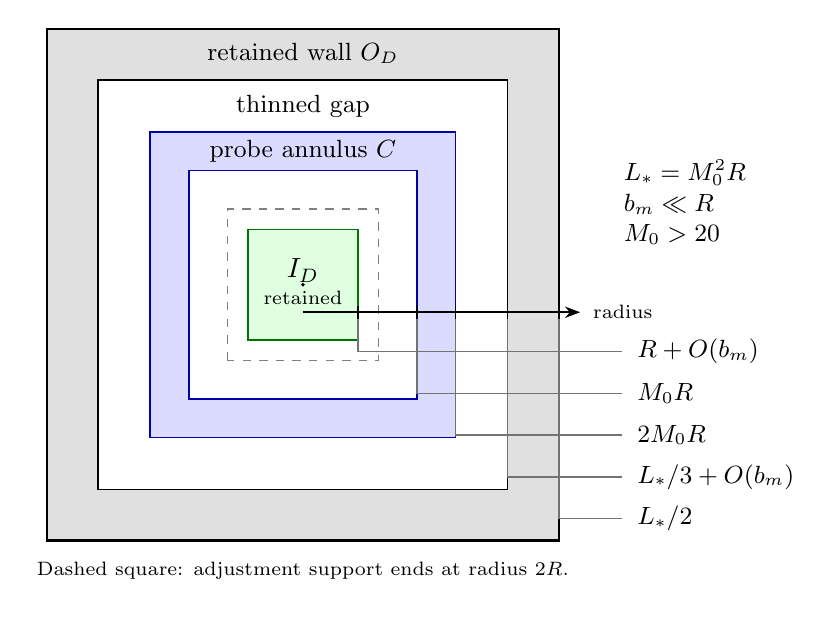
\begin{tikzpicture}[x=1cm,y=1cm,>=Stealth, line width=0.55pt]
  \fill[black!12,even odd rule]
    (-3.25,-3.25) rectangle (3.25,3.25)
    (-2.60,-2.60) rectangle (2.60,2.60);
  \fill[blue!14,even odd rule]
    (-1.94,-1.94) rectangle (1.94,1.94)
    (-1.45,-1.45) rectangle (1.45,1.45);
  \fill[green!12] (-0.70,-0.70) rectangle (0.70,0.70);
  \draw[thick] (-3.25,-3.25) rectangle (3.25,3.25);
  \draw (-2.60,-2.60) rectangle (2.60,2.60);
  \draw[blue!65!black] (-1.94,-1.94) rectangle (1.94,1.94);
  \draw[blue!65!black] (-1.45,-1.45) rectangle (1.45,1.45);
  \draw[green!45!black] (-0.70,-0.70) rectangle (0.70,0.70);
  \draw[dashed,black!50] (-0.96,-0.96) rectangle (0.96,0.96);
  \node at (0,0.18) {$I_D$};
  \node[font=\scriptsize] at (0,-0.16) {retained};
  \node[font=\small] at (0,2.27) {thinned gap};
  \node[font=\small] at (0,1.69) {probe annulus $C$};
  \node[font=\small] at (0,2.94) {retained wall $O_D$};
  \fill (0,0) circle (0.025);
  \draw[->] (0,-0.35) -- (3.52,-0.35);
  \node[anchor=west,font=\scriptsize] at (3.56,-0.35) {radius};
  \draw (0.70,-0.43) -- (0.70,-0.27);
  \draw (1.45,-0.43) -- (1.45,-0.27);
  \draw (1.94,-0.43) -- (1.94,-0.27);
  \draw (2.60,-0.43) -- (2.60,-0.27);
  \draw (3.25,-0.43) -- (3.25,-0.27);
  \draw[black!55] (0.70,-0.44) -- (0.70,-0.85) -- (4.05,-0.85);
  \draw[black!55] (1.45,-0.44) -- (1.45,-1.38) -- (4.05,-1.38);
  \draw[black!55] (1.94,-0.44) -- (1.94,-1.91) -- (4.05,-1.91);
  \draw[black!55] (2.60,-0.44) -- (2.60,-2.44) -- (4.05,-2.44);
  \draw[black!55] (3.25,-0.44) -- (3.25,-2.97) -- (4.05,-2.97);
  \node[anchor=west,font=\small] at (4.12,-0.85) {$R+O(b_m)$};
  \node[anchor=west,font=\small] at (4.12,-1.38) {$M_0R$};
  \node[anchor=west,font=\small] at (4.12,-1.91) {$2M_0R$};
  \node[anchor=west,font=\small] at (4.12,-2.44) {$L_*/3+O(b_m)$};
  \node[anchor=west,font=\small] at (4.12,-2.97) {$L_*/2$};
  \node[align=left,anchor=west,font=\small] at (3.95,1.05)
    {$L_*=M_0^2R$\\$b_m\ll R$\\$M_0>20$};
  \node[font=\scriptsize,align=center] at (0,-3.63)
    {Dashed square: adjustment support ends at radius $2R$.};
\end{tikzpicture}%
}
\caption{One grid tile in the intermediate system. The annulus is a
square annulus, because all indicated radii use the max norm. The
picture is schematic, not to scale: in the proof $M_0$ is large, so
$R\ll M_0R<2M_0R\ll L_*/3$. Inner and wall boundaries are rounded to
unions of level-$m$ tiles; the probe annulus is not so rounded. On
$\mathcal P_D$, the gap has no cell ports, and the added probes occur
only in the displayed annulus.}
\label{van:geometry-figure}
\end{figure}

\subsection{An adaptive adjustment of the affine data}

For the moment use no artificial probes. Let $S'$ be the intermediate
scattering matrix and let $f=f_N$ be the four-component torus embedding
used to define the affine energy in \cref{screen:limit}. Its chord
distances are globally comparable to shortest Euclidean torus
distances, and its nearest-neighbor increments are bounded. Define
four-component data on the intermediate cell ports by
\begin{equation}\label{van:trace-data}
 F=\frac{f-f(c)}{R},\qquad F_I=\one_I F,
 \qquad
 H^0=\sum_{\nu=1}^{4}
 \tr\!\left[F_{I,\nu}(F_\nu-S'F_\nu S'^*)\right].
\end{equation}
As elsewhere, real scalar data inside a matrix expression denote the
corresponding diagonal matrices. The trace $H^0$ is real, since every
diagonal entry of $S'F_\nu S'^*$ is real.
It is the local first variation of the affine energy: for fixed $S'$,
\[
 \left.\frac{\dd}{\dd t}\mathcal Q_{S'}(f-tRF_I)\right|_{t=0}
       =-2R^2H^0.
\]
Here the perturbation is data on the intermediate ports. The proof below
extends it by a cutoff to site data with bounded increments and chooses
its sign separately in each grid tile. On the selector event, the
affected ports disappear in the complementary pass.

\begin{lemma}\label{van:adjustment}
Fix $M_0$. For every $a>0$, one can arrange
\begin{equation}\label{van:adjustment-small}
 \E\bigl[\one_{\mathcal P}|H^0|\bigr]\leq a
\end{equation}
by taking $n$, then $m>n$, then $N$ sufficiently large. More precisely,
the estimate holds for all sufficiently large $n$, all sufficiently
large $m$ depending on $n$, and all sufficiently large $N$ depending on
the fixed pair $(n,m)$.
\end{lemma}

\begin{proof}
For each grid tile choose a cutoff $\eta_D$ that is one on $I_D$,
vanishes at radius $2R$, and has Lipschitz constant at most $C/R$.
Such cutoffs exist once $b_m/R$ is small. Define $H_D^0$ by
\cref{van:trace-data} with $D$ as the test tile, and set
\[
 \varphi(x)=-\sum_D
   \one_{\mathcal P_D}\operatorname{sgn}(H_D^0)
   \eta_D(x)\bigl(f(x)-f(c_D)\bigr),
 \qquad \operatorname{sgn}(0)=0.
\]
The supports are disjoint. On each support, $|f-f(c_D)|\leq CR$,
so the product has uniformly bounded nearest-neighbor increments.
Across support boundaries the same bound holds because the cutoff
vanishes there. Using a shortest lattice path and global comparability
of chord distances gives
\begin{equation}\label{van:adjustment-lipschitz}
 |\varphi(x)-\varphi(y)|\leq C|f(x)-f(y)|
 \quad\text{for all torus sites }x,y.
\end{equation}

This random adjustment is admissible at the start of the complementary
pass in \cref{hier:comparison}. The selector events may be used as
pre-information. Also $S'$ uses the calibrated reference value at every
still-open root, not the hidden true value at that root. By
\cref{hier:hidden}, the disjoint eligible cells and their recorded
statuses do not expose any of those hidden values. Thus $H_D^0$ and
its sign are measurable with respect to the allowed pre-information.
The adjustment does not use the subsequent thinning marks.

On $\mathcal P_D$, all intermediate ports meeting $\supp\eta_D$ lie
in $I_D$, where $\eta_D=1$. No final port meets this support. Hence
$g=f+t\varphi$, $0<t<1$, agrees with $f$ on the final stage-$m$
ports. By symmetry and unitarity of $S'$, the quadratic energy expands as
\[
 \mathcal Q_{S'}(g)=\mathcal Q_{S'}(f)
 +2t\sum_\nu\tr\!\left[
     \varphi_\nu(f_\nu-S'f_\nu S'^*)\right]
 +t^2\mathcal Q_{S'}(\varphi).
\]
One may subtract $f_\nu(c_D)$ in the trace belonging to a fixed tile,
because $S'$ is unitary. Its linear contribution is therefore
$-2tR^2\one_{\mathcal P_D}|H_D^0|$. There are $b_N^2/L_*^2$ grid
tiles. Averaging the uniformly selected test tile and dividing by the
torus area yields
\begin{equation}\label{van:adjustment-expansion}
 \frac{\E\mathcal Q_{S'}(g)}{b_N^2}
 =\frac{\E\mathcal Q_{S'}(f)}{b_N^2}
 -2tM_0^{-4}\E[\one_{\mathcal P}|H^0|]
 +t^2\frac{\E\mathcal Q_{S'}(\varphi)}{b_N^2}.
\end{equation}
By \cref{van:adjustment-lipschitz}, the last energy is at most a
constant times $\mathcal Q_{S'}(f)$.

Apply \cref{hier:comparison,hier:charges} to the first pass with data
$f$. Then apply the comparison to the complementary pass with data
$g$, using the pointwise increment bound for $g$ obtained from
\cref{van:adjustment-lipschitz}. The allowed increment constant is
uniform for $0<t<1$. The fixed-stage affine limits give
\begin{align*}
 b_N^{-2}\E\mathcal Q_{S'}(f)
   &\leq d_n+\varepsilon_n+o_{n,m;N}(1),\\
 b_N^{-2}\E\mathcal Q_{S'}(g)
   &\geq d_m-\varepsilon_n-o_{n,m;N}(1),
\end{align*}
where $\varepsilon_n\to0$ uniformly in $m>n$. Here and below,
$o_{n,m;N}(1)$ tends to zero as $N\to\infty$ with $n,m$ fixed.
Boundedness of $d_n$ now gives, from
\cref{van:adjustment-expansion},
\begin{equation}\label{van:adjustment-inequality}
 2tM_0^{-4}\E[\one_{\mathcal P}|H^0|]
 \leq Ct^2+d_n-d_m+2\varepsilon_n+o_{n,m;N}(1).
\end{equation}
First take $t$ sufficiently small that the quadratic contribution,
after division by $2tM_0^{-4}$, is less than $a/2$. Since $d_n$ is
convergent, the remaining terms are less than the required tolerance
for sufficiently large $n,m,N$ in the stated order. This proves
\cref{van:adjustment-small}.
\end{proof}

\subsection{An annulus of artificial probes}

Add probes at all sites of
\[
 C=\{x:M_0R\leq |x-c|_\infty\leq 2M_0R\},
\]
and nowhere else, using strength $\tau\vartheta(v_x)$, where
\begin{equation}\label{van:probe-scale}
 \tau=\frac{C_0}{R}.
\end{equation}
The constant $C_0$ will be fixed before $n,m,N$ are chosen. For
sufficiently large $m$, \cref{van:scales} implies
$\tau\leq e^{-c_*b_m}$, so this mask is allowed throughout the first
comparison pass. Use the same underlying hierarchy choices as before.
The resulting intermediate scattering matrix has block form
\begin{equation}\label{van:block}
 S=\begin{pmatrix}A&T\\T^\top&B\end{pmatrix}.
\end{equation}
The first block consists of all cell ports, and the second consists of
the new probes. We also use $C$ for their index set. In this section
$I$ denotes the cell ports in the retained inner square and $J$ denotes
all other cell ports; these symbols are local to this section. On
$\mathcal P$, every port in $J$ is outside the probe annulus toward
the exterior. Set
\[
 K=\norm{T}_{\mathrm{HS}}^2.
\]
The data $F,F_I$ still refer to \cref{van:trace-data}, now restricted
to the cell ports of \cref{van:block}.

We first give the deterministic use of a good annular barrier. A site
is called good for this purpose when $\vartheta(v_x)\geq d_0$, where
$d_0>0$ is fixed sufficiently small. Count only edges with both
endpoints good and lying in a buffered square band strictly inside
$C$, for example with both endpoint radii in
$[1.2M_0R,1.8M_0R]$. Give such an edge cost one, and all other edges
cost zero. Denote by $\ell(x)$ the resulting cost distance from the
region $|x-c|_\infty\geq 2M_0R$. Let $\mathcal B$ be the event
\begin{equation}\label{van:barrier-event}
 \ell(x)\geq\gamma M_0R
 \quad\text{whenever }|x-c|_\infty\leq M_0R,
\end{equation}
where $\gamma>0$ is a sufficiently small fixed constant.

\begin{lemma}\label{van:barrier}
For suitable fixed $d_0,\gamma>0$,
$\PP(\mathcal B^c)\leq C e^{-cM_0R}$. On
$\mathcal B\cap\mathcal P$, for every compatible matrix $D'$ on the
source columns indexed by $J$,
\begin{equation}\label{van:barrier-bound}
 \norm{A_{IJ}D'}_{\mathrm{HS}}
 \leq \frac{C}{M_0R\tau d_0}
       \norm{S_{CJ}D'}_{\mathrm{HS}}.
\end{equation}
The constant includes the fixed factor $\gamma^{-1}$. The same cutoff
argument controls every absorbed output supported where the cutoff
equals one; it requires no norm bound on the exterior resolvent.
\end{lemma}

\begin{proof}
Since $\vartheta$ is positive in the interior of the single-site
support, the iid probability
$p_0=\PP\{\vartheta(v_x)<d_0\}$ tends to zero with $d_0$. If
\cref{van:barrier-event} fails, trim a cheap crossing to the buffered
band and erase its loops. The resulting simple path has length
$j\geq cM_0R$. Choosing $\gamma$ sufficiently small, a fixed positive
fraction of its edges must touch bad sites. Since the path is simple,
a fixed positive fraction of its distinct vertices are bad. There are
at most $C(M_0R)^2 4^j$ candidate paths of length $j$, and at most
$2^{j+1}$ ways to designate a subset of their vertices. Independence
therefore bounds the failure probability by
\[
 C(M_0R)^2\sum_{j\geq cM_0R}4^j2^{j+1}p_0^{c'j}.
\]
For sufficiently small fixed $d_0$, this is exponentially small.

For the deterministic estimate, use the physical inverse $G$ of the
intermediate system with the probes inserted, and set
$u=GY_JD'$. Define
\[
 \chi(x)=\min\{1,\ell(x)/(\gamma M_0R)\}.
\]
It is zero at the $J$ sources and one at $I$. An edge across which
$\chi$ changes is a counted edge; on that edge
$|\chi(x)-\chi(y)|\leq(\gamma M_0R)^{-1}$. Since diagonal terms
commute with $\chi$, the equation for $\chi u$ has only the residual
\[
 q=[G^{-1},\chi]u
\]
and no original source. This residual is supported on the probe sites
at endpoints of changing edges. If $\sigma_x=\tau\vartheta(v_x)$,
write $q=Y_C a$ there. In each matrix entry of the map
$Y_C^\top u\mapsto a$, the conversion introduces
$\sigma_x^{-1/2}\sigma_y^{-1/2}\leq(\tau d_0)^{-1}$.
The vertex degree is bounded, and hence
\begin{equation}\label{van:commutator-source}
 \norm{a}_{\mathrm{HS}}
 \leq \frac{C}{M_0R\tau d_0}
       \norm{Y_C^\top u}_{\mathrm{HS}}.
\end{equation}
By \cref{mat:ward}, the norm of propagation from probe sources to
all absorbed outputs is at most one. Since $\chi=1$ at $I$,
\[
 \norm{Y_I^\top u}_{\mathrm{HS}}
 =\norm{Y_I^\top GY_Ca}_{\mathrm{HS}}
 \leq\norm{a}_{\mathrm{HS}}.
\]
The blocks in \cref{van:barrier-bound} are off diagonal, so replacing
the physical fields by their scattering blocks multiplies both sides
by the same factor $2$. This proves the assertion and also the stated
all-output version of the cutoff argument.
\end{proof}

The next event combines small total transmission with positive internal
jump energy and a bound on transmission weighted by $F$. The weighted
bound is needed because $F$ grows on distant cell ports: small $K$ alone
does not control those coordinate factors in the trace.

\begin{lemma}\label{van:good}
Assume $d>0$. There is a constant $c_1>0$ with the following property.
For every sufficiently small fixed $\kappa>0$, one can choose $M_0$
sufficiently large and finite constants $C_1,C_F$, before choosing
$C_0,n,m,N$, so that the following holds. For any fixed sufficiently
large $C_0$, and then $n,m,N$ sufficiently large successively, an event
$\mathcal G$ of probability at least $1/2$ satisfies
\begin{gather}
 \mathcal G\subset\mathcal P\cap\mathcal B,\qquad
 K\leq\kappa,\label{van:good-transmission}\\
 c_1d\leq
 \sum_{i,j\in I}|F(i)-F(j)|^2|A_{ij}|^2
 \leq C_1,\label{van:good-jumps}\\
 \norm{F_\nu T}_{\mathrm{HS}}\leq C_F
 \quad (1\leq\nu\leq4).\label{van:good-weighted}
\end{gather}
In particular, on this event,
\begin{equation}\label{van:external-small}
 \norm{A_{IJ}}_{\mathrm{HS}}
 +\sum_{\nu=1}^4\norm{A_{IJ}F_\nu|_J}_{\mathrm{HS}}
 \leq \frac{C(\sqrt\kappa+C_F)}{M_0C_0d_0}.
\end{equation}
The right side tends to zero as $C_0$ increases, with all constants
chosen before it kept fixed.
\end{lemma}

\begin{proof}
Fix small exception budgets for each of the following assertions, with
their sum less than $1/2$. All probability bounds are unconditional;
in particular, none of the screening or spatial-average estimates is
conditioned on $\mathcal P$. Let $D_*$ be a finite upper bound for all
$d_n$ after increasing the starting level if necessary.

\emph{Small total transmission to the annulus.}
Choose voltage one on $C$, zero within radius $2R$ and at radii at
least $L_*/4$, with logarithmic ramps in the intervening regions.
For example, as a function of $r=|x-c|_\infty$, the inner ramp is
$\log(r/(2R))/\log(M_0/2)$ and the outer ramp is
$\log((L_*/4)/r)/\log(M_0/8)$. It has a compact profile at scale $R$
and
\begin{equation}\label{van:capacity}
 \int_{\R^2}|\nabla\varphi|^2\,\dd x
 \leq\frac{C}{\log M_0}.
\end{equation}
Indeed the area element for square shells is a constant times
$r\,\dd r$, while the gradient on either ramp is at most
$C/(r\log M_0)$. On $\mathcal P$, all cell-port voltages are zero,
and all probe voltages are one. The intermediate energy is therefore
exactly $K$: each cell-to-probe pair is counted once by the symmetric
energy.

Use \cref{screen:profiles} for the starting stage-$n$ energy and
\cref{hier:comparison,hier:charges} for the first pass. For fixed
$M_0,C_0,n$, with $m,N$ subsequently large, this gives
\[
 \E[\one_{\mathcal P}K]
 \leq \frac{CD_*}{\log M_0}
       +o_{n\to\infty}(1)
       +o_{m,N\to\infty;n,M_0,C_0}(1).
\]
Choose $M_0$ large enough for the first term to meet the assigned
Markov bound at threshold $\kappa$, then take $n,m,N$ large in order.
Together with \cref{van:no-large-bound}, this proves
\cref{van:good-transmission} outside the assigned exception.

\emph{Internal jump energy.}
Inside $I$, the intermediate system has exactly the same data as the
full stage-$n$ system without artificial probes. Consider a deep square
of radius $R/4$ and its bounded-jump neighborhoods. A shield at fixed
relative radii inside $I$ has intact stage-$n$ tests. By
\cref{screen:projected,screen:paths}, comparison across that shield
changes the relevant scattering block by at most
$C_n e^{-c_nR^\alpha}$ in operator norm outside an event of vanishing
probability. The block ranks grow only polynomially in $R$.

Fix $n$ with $d_n\geq d/2$. By \cref{screen:limits}, choose a finite
jump cutoff capturing the spatial average on this deep square up to,
say, a quarter of $d_n$. For sufficiently large $m,N$, that truncated
average exceeds $d_n/2$ with the prescribed high probability. Every
such jump lies in $I$. Its squared chord length under $F$ is its
squared physical length divided by $R^2$, up to factors tending to
one as $b_N/R\to\infty$. The deep square has area comparable to
$R^2$. The preceding operator-norm comparison incurs a vanishing
error in the resulting weighted sum, because the rank is polynomial
and the shield error is exponential. This gives the lower bound in
\cref{van:good-jumps}, with $c_1>0$ independent of the later scales.

For the upper bound, extend $F|_I$ to data vanishing by radius $2R$,
with Lipschitz constant $C/R$. Apply the coarse profile bound in
\cref{screen:profiles} and then the first-pass comparison. The
expected intermediate energy is at most $CD_*+o(1)$. The sum of
internal jump terms is at most twice this energy. Markov's inequality
therefore gives a fixed upper cutoff $C_1$, chosen before $C_0$, for
the assigned exception budget.

\emph{Weighted transmission.}
For cell ports within a sufficiently large absolute multiple of
$L_*$ from $c$, chord bounds give $|F_\nu|\leq CM_0^2$. Their
contribution to $\norm{F_\nu T}_{\mathrm{HS}}$ is at most
$CM_0^2\sqrt K$. Beyond this range, retain only the good-edge costs
on the thick grid walls $O_D$. Those costs are still available in the
intermediate system, including their buffered tests. The wall estimate
in \cref{screen:walls}, followed by
\cref{screen:projected}, gives for a dyadic distance range of order
$D_1$ the expectation bound
\begin{equation}\label{van:far-weighted}
 C_{n,M_0}R^2(D_1/R)^2
 \left(e^{-c_nD_1^\alpha}+D_1^{-30}\right).
\end{equation}
To see the rank factor, there are $O_{M_0}(R^2)$ input probes; the
operator norm of transmission across a successful wall shield is
exponentially small, and it is always at most one by unitarity. The
chord weight is at most $CD_1/R$. At torus-size distances one uses a
separating band with radius a sufficiently small fixed multiple of
$D_1$, so the same estimates apply. The dyadic sum of
\cref{van:far-weighted} tends to zero as $m$ increases at fixed $n$,
uniformly for sufficiently large $N$: its polynomial part is a sum
of $D_1^{-28}$. Thus one may choose, for example,
$C_F=CM_0^2\sqrt\kappa+1$, with a sufficiently large absolute
constant and harmless extra slack for all four components. This
choice is independent of $n,C_0$; only the scale required to make the
far error small depends on them.

Finally include $\mathcal B$ using \cref{van:barrier}. The total
exception probability is less than $1/2$. This proves the event
assertion. Apply \cref{van:barrier-bound} with $D'=1$ and with
$D'=F_\nu|_J$. Since $S_{CJ}=(T^\top)_{CJ}$,
its unweighted Hilbert-Schmidt norm is at most $\sqrt K$, and its
weighted norm is at most $\norm{F_\nu T}_{\mathrm{HS}}$.
Substituting \cref{van:probe-scale} proves
\cref{van:external-small}.
\end{proof}

\subsection{An analytic trace with nonzero central value}

Close all inserted probes with the common phase $z$. For real $s$,
the corresponding physical shifts and the phase are
\begin{equation}\label{van:twist-parameter}
 v_x\longmapsto v_x+s\vartheta(v_x)\quad (x\in C),
 \qquad z=\frac{s+i\tau}{s-i\tau}.
\end{equation}
By \cref{mat:closure}, the scattering matrix on cell ports is
\begin{equation}\label{van:closed-family}
 S_z=A+\Delta(z),\qquad
 \Delta(z)=Tz(1-zB)^{-1}T^\top.
\end{equation}
Define $H(z)$ on the unit circle by replacing $S'$ with $S_z$ in
\cref{van:trace-data}. Its matrix expression contains the adjoint
$S_z^*$. To remove that obstruction to analyticity, replace the adjoint
by the adjugate and multiply the constant term by the determinant:
\begin{equation}\label{van:analytic-function}
 \mathfrak h(z)=\sum_\nu\tr\!\left[
 F_{I,\nu}\{F_\nu\det S_z-S_zF_\nu\operatorname{adj}S_z\}\right]
\end{equation}
This function is analytic in the disk. Indeed $B$ is a contraction, and the
scattering entries in \cref{van:closed-family} are rational analytic
functions there. Possible boundary poles are removable: away from
finitely many points their boundary values are unitary, which excludes
a genuine pole of a rational entry on the circle. Thus
$\mathfrak h$ extends continuously to the boundary. There,
\begin{equation}\label{van:boundary-modulus}
 \mathfrak h(z)=\det(S_z)H(z),\qquad
 |\mathfrak h(z)|=|H(z)|,
\end{equation}
because $\operatorname{adj}S_z=(\det S_z)S_z^*$.

\begin{lemma}\label{van:analytic-bounds}
Choose $\kappa$ sufficiently small depending on $d$, then the
constants in \cref{van:good}, and then $C_0$ sufficiently large.
There are constants $c_2>0$ and $B_p<\infty$, independent of the
later choices $n,m,N$, such that on $\mathcal G$
\begin{equation}\label{van:central-bound}
 |\mathfrak h(0)|\geq c_2,
\end{equation}
and, for every fixed $0<p<1/2$,
\begin{equation}\label{van:hardy-bound}
 \int_{\T}|H(z)|^p\,\dd\gamma_{\T}(z)\leq B_p.
\end{equation}
Here $\gamma_{\T}$ is normalized Haar measure. Neither constant
depends on the number of cell ports or probes.
\end{lemma}

\begin{proof}
Unitarity in \cref{van:block} gives $AA^*=1-TT^*$. If the
eigenvalues of $TT^*$ are $\delta_j\geq0$, then
$\sum_j\delta_j=K\leq\kappa$. Thus $A$ is invertible and
\begin{equation}\label{van:almost-unitary}
 |\det A|^2=\prod_j(1-\delta_j)\geq1-K,
 \qquad
 \norm{A^{-1}-A^*}_1
 =\norm{A^{-1}TT^*}_1
 \leq\frac{K}{\sqrt{1-K}}\leq2K
\end{equation}
for sufficiently small $\kappa$. At zero,
\begin{equation}\label{van:central-trace}
 \frac{\mathfrak h(0)}{\det A}
 =\sum_\nu\tr\!\left[F_{I,\nu}
                      (F_\nu-AF_\nu A^{-1})\right].
\end{equation}
On $I$ every $F_\nu$ is bounded by an absolute constant, because
the radius of $I$ is $R+O(b_m)$.

First retain only the $I,I$ indices in the product term of
\cref{van:central-trace}, along with the entire constant trace.
Replacing the internal block of $A^{-1}$ by that of $A^*$ costs at
most $CK$ in trace norm, by \cref{van:almost-unitary}. Symmetry of
$A$ makes the resulting internal expression exactly
\begin{equation}\label{van:internal-positive}
 \frac12\sum_{i,j\in I}|A_{ij}|^2|F(i)-F(j)|^2
 +\sum_{i\in I}|F(i)|^2
                  \left(1-\sum_{j\in I}|A_{ij}|^2\right).
\end{equation}
The second term is nonnegative, since $A$ is a contraction. The
first is at least $c_1d/2$ on $\mathcal G$.

For the external part, put
\[
 \delta_A=\norm{A_{IJ}}_{\mathrm{HS}}
       +\sum_\nu\norm{A_{IJ}F_\nu|_J}_{\mathrm{HS}}.
\]
Symmetry and \cref{van:almost-unitary} give
\[
 \norm{(A^{-1})_{JI}}_{\mathrm{HS}}
 \leq\norm{A_{IJ}}_{\mathrm{HS}}+2K.
\]
The external trace is consequently bounded in modulus by
$C\delta_A(\delta_A+K)$. Choose $\kappa$ so that the internal
replacement error is less than $c_1d/8$. After the choices in
\cref{van:good}, choose $C_0$ so large that
\cref{van:external-small} makes the external error less than
$c_1d/8$. The real part of \cref{van:central-trace} is then at
least $c_1d/4$. Combining with $|\det A|\geq\sqrt{1-\kappa}$
proves \cref{van:central-bound}.

For the boundary moment, expand the trace using $S_z=A+\Delta$.
The part $H_A$ with $A,A^*$ has a bounded modulus on $\mathcal G$.
Indeed its internal part is \cref{van:internal-positive}, whose
first term is bounded by $C_1/2$, and
\[
 \sum_{i\in I}\left(1-\sum_{j\in I}|A_{ij}|^2\right)
 \leq K+\norm{A_{IJ}}_{\mathrm{HS}}^2.
\]
The external part is bounded using
\cref{van:external-small}. All these bounds involve only the fixed
cutoffs in \cref{van:good}.

Consider a linear term, for one component,
\[
 \tr(F_I\Delta F A^*)
 =\tr\!\left[z(1-zB)^{-1}D_F\right],
 \qquad D_F=T^\top F A^*F_I T.
\]
Its coefficient satisfies
\[
 \norm{D_F}_1
 \leq\norm{T^\top F A^*}_{\mathrm{HS}}
       \norm{F_I T}_{\mathrm{HS}}
 \leq\norm{FT}_{\mathrm{HS}}
       \norm{F_I T}_{\mathrm{HS}}.
\]
The other linear term is its complex conjugate on the circle.
By \cref{mat:weak}, these terms have weak $L^1$ bounds depending
only on $C_F$ and $\kappa$, since
$\norm{F_I T}_{\mathrm{HS}}\leq C\sqrt\kappa$.

The quadratic term is bounded by
\[
 |\tr(F_I\Delta F\Delta^*)|
 \leq\norm{F_I\Delta}_{\mathrm{HS}}
       \norm{\Delta F}_{\mathrm{HS}}.
\]
Again \cref{mat:weak}, with the respective sandwiches
$(F_I T,T^\top)$ and $(T,T^\top F)$, gives weak $L^1$ bounds for
each factor. A nonnegative random variable with weak $L^1$ bound
$a$ has every moment $q<1$ bounded by $C_q a^q$, by integration
of its tail. Applying Cauchy--Schwarz with exponent $2p<1$ therefore
bounds the $p$-moment of this product. There are four components and
finitely many terms. Subadditivity at exponent $p<1$ proves
\cref{van:hardy-bound}. The use of Hilbert-Schmidt products and
trace norms makes the bounds independent of all matrix dimensions.
\end{proof}

\subsection{Changing the potential law under a bounded twist}

The artificial profile vanishes at the support endpoints and belongs
to $C^{1,1}([-h,h])$. For sufficiently small $|s|$, the map
\[
 T_s(v)=v+s\vartheta(v)
\]
is therefore a diffeomorphism of $[-h,h]$ onto itself, with derivative
at least $1/2$. If $r_s$ is the density of its pushforward of the
uniform law relative to that same law, then
\[
 r_s(y)=\frac{1}{1+s\vartheta'(T_s^{-1}(y))},
 \qquad |r_s-1|\leq C|s|,\qquad \int r_s\,\dd\mu=1.
\]
Consequently
\begin{equation}\label{van:single-density}
 \int r_s^2\,\dd\mu
 =1+\int(r_s-1)^2\,\dd\mu\leq1+Cs^2.
\end{equation}
Here $\mu$ is the uniform law on $[-h,h]$.

Fix $W<\infty$ and assume $|s|/\tau\leq W$. Conditional on the
offset and the test tile, change every true variable in $C$ by $T_s$
and leave all other true variables, selectors, and auxiliary uniforms
unchanged. There are at most $C(M_0R)^2$ changed sites. By independence
and \cref{van:single-density}, the resulting joint law has a density
$\mathscr D_s$ relative to the original joint law with
\begin{equation}\label{van:joint-density}
 \norm{\mathscr D_s}_{L^2}^2
 \leq \exp(CM_0^2R^2s^2)
 \leq \exp(CM_0^2C_0^2W^2)=D_W^2.
\end{equation}
This also holds after averaging over the offset and the test tile.
The bound is uniform in $m,N$ once they are sufficiently large for
the maps to be diffeomorphisms. Its constant may be large; only its
independence of the later scales matters.

We next check why this change of true potentials reproduces the
closed-probe system despite the potential-dependent hierarchy.
This check concerns recomputed statuses, not an assumption that
statuses are fixed by definition.

On $\mathcal P$, selected tiles of level at least $m$ do not meet
the test tile. Every tile of level below $m$ touching $C$ lies wholly
in the thinned gap, since $b_m\ll R$ and the annulus is separated
from both retained regions by a distance comparable to $R$. Thus a
selected tile capable of carrying an intermediate cell port is
disjoint from $C$. Its own true variables, own corner labels, local
likelihood, and reference potential are unchanged by the shift.
Eligibility depends only on selectors and is unchanged as well.

There is one remaining possibility: a changed coordinate may alter
the validity of an ancestor label used by a retained tile. Any such
ancestor contains both the retained root and a coordinate in $C$.
Their separation is at least a fixed multiple of $R$, so the ancestor
side is at least $cR$. The probability that any such large tile has
an invalid own label is bounded by
\begin{equation}\label{van:gate-exception}
 u_R=C_{M_0}\sum_{b_l\geq cR}(1+R/b_l)^2b_l^{-K_0}=o(1).
\end{equation}
This counts only tiles meeting $C$, which also covers every relevant
changed triple. The original bound is uniform in the offset and
torus size. After the shift the probability is at most
$D_W\sqrt{u_R}$ by \cref{van:joint-density}. Exclude both events.
All potentially changed ancestor validity tests are then valid before
and after the shift. Ancestor box identities themselves need not be
the same: the acceptance rules use those identities only through the
validity gates, whereas each retained tile's own box and likelihood
are unchanged.

On the remaining part of $\mathcal P$, all intermediate cell ports
and references are therefore unchanged when the hierarchy is
recomputed with the same selectors and auxiliary uniforms. Changes
of acceptance inside the gap have no effect, because those ports
have already been thinned, and $\mathcal P$ excludes the larger
ones. Before closure the real potentials on $C$ were the true ones;
the only added terms there were the artificial absorbers. Hence
\cref{mat:closure,van:twist-parameter} imply that $H(z)$ is exactly
the no-extra-probe intermediate trace $H^0$ evaluated at the shifted
data. Almost-everywhere inverse statements suffice throughout.

Let $a_{n,m,N}=\E[\one_{\mathcal P}|H^0|]$ in the original law.
Since $\mathcal P$ uses only unchanged selectors, Markov's inequality
and \cref{van:joint-density} give, for every fixed $\delta>0$,
\begin{equation}\label{van:twist-probability}
 \PP\{\mathcal G,\ |H(z)|>\delta\}
 \leq e_R(W)+D_W\left(\frac{a_{n,m,N}}{\delta}\right)^{1/2},
 \qquad |s|/\tau\leq W,
\end{equation}
where one may take $e_R(W)=u_R+D_W\sqrt{u_R}$. This tends to zero
as $m$ grows at fixed $W,M_0,C_0$. The estimate is uniform over
bounded twists; it does not assert simultaneous invariance for all
twists on a single realization. Only the probability bound for each
twist will be integrated.

\subsection{The contradiction}

\begin{proof}[Proof of \cref{van:zero}]
Retain the assumption $d>0$. Choose the constants in the following
order. First fix the barrier constants $d_0,\gamma$, then choose
$\kappa$ small enough for \cref{van:analytic-bounds}. Choose $M_0$
and the cutoffs $C_1,C_F$ using \cref{van:good}. Then choose $C_0$
sufficiently large for the same analytic lemma. All these choices
precede $n,m,N$. They provide a fixed central lower bound $c_2>0$
and a fixed boundary moment bound $B_p$ on an event $\mathcal G$
of probability at least $1/2$ once those scales are sufficiently large.

Fix $0<p'<p<1/2$. Under Haar measure, $s/\tau$ in
\cref{van:twist-parameter} has the standard Cauchy law. Denote its
tail probability beyond $W$ by $\beta_W$, so $\beta_W\to0$.
Apply H\"older's inequality on the product of the underlying
probability space and the circle. The pointwise good-data bound
\cref{van:hardy-bound} gives
\begin{align}
 &\E\left[\one_{\mathcal G}
        \int_\T |H(z)|^{p'}\,\dd\gamma_\T(z)\right]
 \label{van:small-boundary}\\
 &\quad\leq \delta^{p'}
   +B_p^{p'/p}\left[
       \beta_W^{1-p'/p}
       +\left\{e_R(W)+D_W
          \left(\frac{a_{n,m,N}}{\delta}\right)^{1/2}
        \right\}^{1-p'/p}\right].\notag
\end{align}
For completeness, the first term covers $|H|\leq\delta$. The
Haar tail costs the first H\"older term. On the bounded-twist part,
\cref{van:twist-probability} bounds the product measure of
$\{\mathcal G,|H|>\delta\}$, and the same $p$-moment bound gives
the second H\"older term. Tonelli's theorem applies to these
nonnegative quantities; no realization-wise uniformity in the twist
is used.

The right side can be made smaller than $c_2^{p'}/4$. To see the
order without interchanging limits, first choose $W$ so the tail term
is small, then choose $\delta$ so $\delta^{p'}$ is small. With these
fixed, $D_W$ is a fixed finite constant. Choose the tolerance in
\cref{van:adjustment} sufficiently small relative to $D_W$ and
$\delta$. Take $n$ large for that adjustment and the good-data
requirements; then take $m$ large for all fixed-$n$ spatial estimates,
the probe-strength constraint, and $e_R(W)$; finally take $N$ large
for the finite-torus approximations at this fixed pair. Increasing
$m,N$ as required preserves the preceding assertions. Thus
\cref{van:small-boundary} is indeed less than $c_2^{p'}/4$.

On the other hand, $|\mathfrak h|^{p'}$ is subharmonic in the disk.
For example, one may first use the nonnegative Laplacian of
$(|\mathfrak h|^2+\epsilon)^{p'/2}$ and then let
$\epsilon\downarrow0$. The continuous boundary extension and
\cref{van:boundary-modulus,van:central-bound} give on every good
realization
\[
 \int_\T|H(z)|^{p'}\,\dd\gamma_\T(z)
 =\int_\T|\mathfrak h(z)|^{p'}\,\dd\gamma_\T(z)
 \geq |\mathfrak h(0)|^{p'}\geq c_2^{p'}.
\]
Taking the expectation over $\mathcal G$ gives a lower bound
$c_2^{p'}/2$, contradicting the preceding upper bound. Therefore
$d=0$.
\end{proof}

\section{A fixed-energy fractional-moment estimate}
\label{sec:bootstrap}

We return to the true product law and remove the hierarchy from the
operator whose decay is to be estimated. Throughout this section,
\(h>0\) and \(E\in(-4-h,4+h)\) are fixed. All choices may depend on
these two parameters. Distance means the shortest-coordinate max-norm
distance on the torus \(\T_N^2=(\Z/b_N\Z)^2\). The notation for the probe
sets below is local to this section.

\begin{theorem}[True torus Green function]\label{boot:fractional}
Fix \(0<s<1/16\). There are constants
\(A=A(h,E,s)<\infty\), \(a=a(h,E,s)>0\), and an integer
\(N_0=N_0(h,E,s)\) such that, for every \(N\ge N_0\) and every
\(x,y\in\T_N^2\),
\begin{equation}\label{boot:real-decay}
 \E\abs{(H_N-E)^{-1}_{xy}}^{s/2}
       \le A\exp\{-a\dist(x,y)\}.
\end{equation}
Here \(H_N\) has the true iid uniform \([-h,h]\) diagonal and periodic
nearest-neighbor hopping. Its inverse at the specified real energy
exists almost surely. No uniformity in \(E\), nor any statement about
time evolution, is part of this theorem.
\end{theorem}

We prove the theorem by first retaining arbitrary deterministic masks of
artificial probes. At each site a mask prescribes absence, strength
\(\tau\), or strength \(\tau\vartheta(v_i)\), with at most one probe per
site. The profile \(\vartheta\) is the one fixed earlier; in particular
it equals one on \([-h/2,h/2]\), is \(C^{1,1}\), and vanishes quadratically
only at the endpoints of the potential interval. Write
\(\eta_i\) for a prescribed positive probe strength and let \(Y\) have
columns \(\sqrt{\eta_i}e_i\). In this section
\[
 G=(H_N-E-iYY^\top)^{-1},\qquad S=1+2iY^\top GY.
\]
Thus \(S\) is symmetric and unitary, and \(Y^\top GY\) is a
contraction by \Cref{mat:ward}. All exceptional algebraic singularities
below can be discarded under the continuous product law.

The parameter order is
\begin{equation}\label{boot:order}
 s,\ d_0,\ C_0,\ n,\ m,\ N,
 \qquad R=\lfloor\exp(b_m^2)\rfloor,\qquad \tau=C_0/R.
\end{equation}
The barrier threshold \(d_0>0\) will be small; \(C_0\) will be large.
After they have been fixed, \(n\) and then \(m>n\) are made sufficiently
large. Finally \(N\) is sufficiently large in terms of all these
choices; all ensuing estimates hold for every larger \(N\). We always
require \(b_N>100R\) and \(\tau\le1\).

\subsection{Filling and twisting an annulus}

Let \(X,Y'\) be arbitrary deterministic subsets of the probe sites in
the radius-\(R\) squares centered at \(x,y\), respectively, where
\(\dist(x,y)\ge10R\). Let
\[
 C=\{i:2R\le\dist(i,x)\le4R\}.
\]
Fill every previously unoccupied site of \(C\) with a probe of strength
\(\tau\vartheta(v_i)\), keeping existing probes and their strengths.
The filled mask is again deterministic. Superscripts \({\rm old}\) and
\({\rm fill}\) distinguish the resulting scattering matrices. Identify
the probes in \(C\) with their sites and put
\[
 U=\norm{S^{\rm fill}_{CX}}_{\rm HS},\qquad
 V=\norm{S^{\rm fill}_{CY'}}_{\rm HS},\qquad
 D=\norm{S^{\rm fill}_{Y'X}}_{\rm HS}.
\]

\begin{lemma}[Mixture domination]\label{boot:twist}
There is \(C_s<\infty\), independent of the masks, centers, \(R,N\),
and \(C_0\ge1\), such that
\begin{equation}\label{boot:twist-ineq}
 \E\norm{S^{\rm old}_{Y'X}}_{\rm HS}^{s}
     \le C_s(1+C_0)\E\bigl[D^s+V^sU^s\bigr].
\end{equation}
As everywhere in this section, the constant may depend on the fixed
\(h,E,s\) and profile.
\end{lemma}

\begin{proof}
Close just the newly added probes using a common Haar phase \(z\).
The closure identity in \Cref{mat:closure} and the sandwich estimate in
\Cref{mat:weak}, followed by integration of the weak \(L^1\) tail, give
\[
 \int\norm{(S_z)_{Y'X}}_{\rm HS}^{s}\,\dd z
       \le C_s(D^s+V^sU^s).
\]
Here \(\dd z\) is normalized Haar measure, and the blocks linking the
new probes to \(X,Y'\) are subblocks of those defining \(U,V\).
The corresponding real closing shift at each newly occupied site is
\(w\vartheta(v_i)\), where \(w\) has density
\[
                 \frac{\tau}{\pi(w^2+\tau^2)}.
\]
Only newly occupied sites are shifted, so after closing we have precisely
the old mask evaluated at these shifted true potentials.

For \(\abs w\le c/R\), with fixed sufficiently small \(c>0\), the map
\(T_w(v)=v+w\vartheta(v)\) is a diffeomorphism of \([-h,h]\) onto
itself. If \(u=T_w(v)\), its pushforward density relative to the uniform
law is \(r_w(u)=(1+w\vartheta'(v))^{-1}\). Uniformly in \(u\),
\[
 \log r_w(u)=-w\vartheta'(u)+O(w^2).
\]
This follows from the inverse Jacobian and the Lipschitz continuity of
\(\vartheta'\). There are at most \(K R^2\) shifted sites, so at each
fixed output configuration the joint density satisfies
\[
 \log\prod_i r_w(u_i)
        =-w\sum_i\vartheta'(u_i)+O(R^2w^2).
\]
Choose the half interval \([0,c/R]\) or \([-c/R,0]\) on which the linear
term is nonnegative. On this entire half interval the joint density is
at least a fixed positive constant. Its Cauchy probability is
\[
 \frac1\pi\arctan\frac c{C_0}\ge\frac{c_1}{1+C_0}.
\]
Consequently the full shifted mixture dominates
\(c_2(1+C_0)^{-1}\) times the true product law, pointwise in the output
configuration. Applying this domination to the nonnegative old-mask
block power and then averaging the Haar estimate proves the claim.
\end{proof}

We seek a bound by an arbitrarily small multiple of \(\E V^s\).
Thus \Cref{boot:twist-ineq} leaves two tasks: attenuate \(D\) across
the filled annulus, and combine a small mean return \(U\) with a
resampling bound for \(U^sV^s\). An unweighted estimate for barrier
failure would not suffice when \(\E V^s\) is small. We therefore
control that failure also under the \(V^s\)-weighted law.

\subsection{Two barriers under a transmission tilt}

Call a site good when \(\vartheta(v_i)\ge d_0\). Give cost one to an
edge precisely when both endpoints are good and both radii about \(x\)
belong to \([2.2R,2.8R]\); all other edges have cost zero. Let
\(d_{\rm in}\) be the associated path-cost distance from the radius-\(2R\)
square. Independently of this definition, count good-good edges with
both radii in \([3.2R,3.8R]\), and let \(d_{\rm out}\) be the resulting
distance from \(\{i:\dist(i,x)\ge4R\}\). Integer roundings of the four
band boundaries make no difference to the constants. For a sufficiently
small absolute \(\gamma>0\), define
\begin{equation}\label{boot:barrier-event}
 \mathcal B=\left\{
 \begin{array}{ll}
 d_{\rm in}(i)\ge\gamma R&\text{if }\dist(i,x)\ge3R,\\
 d_{\rm out}(i)\ge\gamma R&\text{if }\dist(i,x)\le3R.
 \end{array}\right\}.
\end{equation}
These two strictly buffered bands will allow separate resampling of the
inside and outside of radius \(3R\).

\begin{lemma}[Uniform one-site estimates under tilt]\label{boot:tilted}
Suppose \(\E V^s>0\), and define the probability law
\[
                      \dd\nu=\frac{V^s}{\E V^s}\,\dd\PP.
\]
For a site \(i\in C\), conditional on all other potentials, put
\(W(v_i)=V^s\). Then
\begin{equation}\label{boot:l2l1}
       \bigl(\E_i W^2\bigr)^{1/2}\le K_s\E_i W,
\end{equation}
with a constant uniform in every frozen exterior and in the mask.
For \(d_0>0\) sufficiently small, chosen after \(s\) and before \(C_0\),
there are \(K,c>0\) such that
\begin{equation}\label{boot:tilted-barriers}
 \PP(\mathcal B^c)+\nu(\mathcal B^c)\le K e^{-cR},
 \qquad
 \E_\nu d_{\min}^{-2s}\le K R^2,
 \qquad d_{\min}=\min_{i\in C}\vartheta(v_i).
\end{equation}
No independence under \(\nu\) is asserted or needed.
\end{lemma}

\begin{proof}
Fix all variables except \(v=v_i\), and write the probe factor at \(i\)
as \(a(v)\in\{1,\vartheta(v)\}\). Schur complementation at \(i\)
expresses the other rows and the row at \(i\) of the block defining \(V\)
in the form
\[
 A'+\frac{D'}{v-i\tau a(v)-w_*},\qquad
 \frac{D''\sqrt{a(v)}}{v-i\tau a(v)-w_*},\qquad \Im w_*\ge0.
\]
The coefficients are fixed matrices of compatible sizes. Passivity
gives the sign of \(\Im w_*\). The deleted physical-site system is
invertible almost surely: the imaginary part forces a kernel vector to
vanish at all remaining probe sites, so it would lie in the kernel of
the true real restriction, whose nonzero determinant polynomial
vanishes only on a product-law null set.
Writing both rows over their common denominator, their joint numerator is
\[
 N(v)=\bigl((v-i\tau a(v)-w_*)A'+D',\ D''\sqrt{a(v)}\bigr).
\]
On the plateau \(P=[-h/2,h/2]\), this is the affine vector
\(N_P(v)=(vA'+B,D'')\), where \(B=D'-(i\tau+w_*)A'\).
If \(M=\max_{v\in P}\norm{N_P(v)}_{\rm HS}\), then
\[
 \norm{A'}_{\rm HS}\le2M/h,\qquad
 \norm{(B,D'')}_{\rm HS}\le M,\qquad
 \sup_{[-h,h]}\norm{N(v)}_{\rm HS}\le K_hM.
\]
Moreover an interval in \(P\) of length at least \(h/4\), adjacent to
an endpoint attaining the maximum, has numerator norm at least \(M/2\).
This uses the displayed slope bound. If \(M=0\), the entire block
vanishes and the claimed inequality is immediate.

Put \(b(v)=v-i\tau a(v)-w_*\). Its modulus is at most
\(K_h(1+\abs{w_*})\). For every \(0<q<1\),
\begin{equation}\label{boot:denominator}
 \E_i\abs{b(v)}^{-q}\le K_{h,q}(1+\abs{w_*})^{-q}.
\end{equation}
Indeed, for bounded \(w_*\) use
\(\abs{b(v)}\ge\abs{v-\Re w_*}\) and integrate the one-dimensional
singularity; for \(\abs{w_*}\) sufficiently large use
\(\abs{b(v)}\ge\abs{w_*}-h-1\). Hence
\[
 \E_i W\ge c_{h,s}\left(\frac M{1+\abs{w_*}}\right)^s,
 \qquad
 \E_i W^2\le K_{h,s}\left(\frac M{1+\abs{w_*}}\right)^{2s}.
\]
This proves \Cref{boot:l2l1}, uniformly even for arbitrarily large
exterior impedance.

For any measurable single-site set \(A\), Cauchy--Schwarz now gives
\[
 \nu(v_i\in A\mid(v_j)_{j\ne i})
       \le K_s\PP(v_i\in A)^{1/2}
\]
whenever the conditional normalizing mean is positive. The remaining
conditional configurations have zero \(\nu\)-measure. In particular
the right side for \(A=\{\vartheta<d_0\}\) tends to zero with \(d_0\),
uniformly in the conditioning. Iterating this estimate over any fixed
set of distinct sites bounds the probability that all of them are bad
by \(\beta^{k}\), where \(\beta\) can be made arbitrarily small.

A failure of either barrier gives, after trimming to intermediate
radii and erasing loops, a simple path in the corresponding band of
length \(j\ge c_3R\) and cost less than \(\gamma R\). For \(\gamma\)
small, a fixed positive fraction of its edges are not good-good.
Since the path is simple, this forces at least \(c_4j\) distinct bad
sites. There are at most \(K R^2 4^j\) candidate paths of length \(j\),
and at most \(2^{j+1}\) subsets of their vertices. Choose \(d_0\) so
that \(8\beta^{c_4}<1\). Summing the resulting geometric series for
\(j\ge c_3R\) proves the tilted exponential bound. The same argument
with the original independent site probabilities proves the untilted
bound.

Finally, the same conditional Cauchy--Schwarz estimate gives
\[
 \E_\nu[\vartheta(v_i)^{-2s}\mid(v_j)_{j\ne i}]
       \le K_s\bigl(\E_i\vartheta(v_i)^{-4s}\bigr)^{1/2}\le K.
\]
The integral is finite because \(\vartheta\) vanishes quadratically and
\(8s<1\). Since
\(d_{\min}^{-2s}\le\sum_{i\in C}\vartheta(v_i)^{-2s}\) and
\(\abs C\le K R^2\), this proves the last assertion.
\end{proof}

\subsection{Cutoffs and the small return estimate}

We record explicitly the consequence of \Cref{van:barrier} that will be
used several times. Suppose \(\Psi=GY_J\) is a matrix of fields sourced
at a probe set \(J\), and a scalar cutoff \(\chi\) changes only across
edges whose two endpoints belong to \(C\) and carry probes of strengths
at least \(\tau d\). If \(\abs{\chi_i-\chi_j}\le L\), then the hopping
commutator can be written as a probe source:
\begin{equation}\label{boot:commutator}
 [H_N,\chi]\Psi=Y_C B_\chi,
 \qquad
 \norm{B_\chi}_{\rm HS}
       \le\frac{K L}{\tau d}
           \norm{Y_C^\top\Psi}_{\rm HS}.
\end{equation}
Only endpoints of changing edges need be included on the right.
Indeed, in the coefficient at an endpoint one divides by its square
root strength, and replaces each neighboring field by its absorbed
field divided by that neighbor's square root strength. Bounded lattice
degree gives the stated operator bound. Ward then yields
\begin{equation}\label{boot:cutoff-ward}
 \norm{Y^\top G[H_N,\chi]\Psi}_{\rm HS}
             \le\norm{B_\chi}_{\rm HS}.
\end{equation}
The output here includes \emph{all} probes. These estimates also compare
two systems agreeing on the cutoff support and its changing edges:
cut off a field of the first system and correct its commutator residual
in the second. No estimate on the exterior resolvent is involved.

\begin{lemma}[Small return to a filled annulus]\label{boot:return}
For each fixed sufficiently large \(C_0\) and each \(\epsilon>0\),
one can choose \(n\), then \(m>n\), then a threshold for \(N\), so that
\[
                          \E U^2<\epsilon
\]
for every subsequent \(N\), every deterministic mask, every center,
and every permitted subset \(X\).
\end{lemma}

\begin{proof}
Carry the filled artificial mask through the auxiliary hierarchy.
Take a scalar voltage \(f_R\) equal to one on the radius-\(R\) square,
zero at radii at least \(2R\), and Lipschitz with constant \(K/R\).
By \Cref{screen:profiles}, at fixed \(n\),
\[
 \E\mathcal Q_{n,N}(f_R)\le Kd_n+o_{m,N;n,C_0}(1).
\]
Apply \Cref{hier:comparison} to thin to uniform stage \(m\).
The profile is supported in the radius-\(2R\) square and has Lipschitz
constant \(K/R\), while \(b_m\ll R\). Thus
\Cref{hier:charges}(ii) bounds its unnormalized charge by \(K r_n\),
where \(r_n=\sum_{l\ge n}q_lp_l\to0\), independently of \(R\).
Writing \(U_m\) for the same artificial-probe block at stage \(m\),
we obtain
\begin{equation}\label{boot:return-stage}
 \E U_m^2
    \le Kd_n+o_{n\to\infty}(1)+o_{m,N;n,C_0}(1).
\end{equation}
Each probe pair contributing to \(U_m^2\) has unit squared voltage difference and is
counted in both directions in \(\mathcal Q\), canceling its factor
\(1/2\). The artificial probes are allowed in the comparison because
\(C_0/R\le\exp(-c_*b_m)\) for sufficiently large \(m\).

Let \(\mathcal A\) be the event that no selected tile of level at least
\(m\) meets the radius-\(5R\) square. Tile counting gives
\[
 \PP(\mathcal A^c)
       \le K\sum_{l\ge m}(1+R/b_l)^2 e^{-b_l^6}
       =o(R^{-4}).
\]
For example each fixed polynomial loss in \(R\) is dominated by
\(\exp(-b_m^6)\), since \(\log R\sim b_m^2\).
On \(\mathcal A\), the stage-\(m\) and true filled coefficients and
probes coincide throughout this square. On \(\mathcal B\) use
\[
                 \chi=(1-d_{\rm in}/(\gamma R))_+.
\]
It equals one on \(X\), vanishes outside radius \(3R\), and changes
only on shared good-good edges. Cut off stage-\(m\) fields sourced at
\(X\), and correct in the true system using
\Cref{boot:commutator,boot:cutoff-ward}. Since \(R\tau=C_0\),
\[
                   U\le\left(1+\frac K{C_0d_0}\right)U_m
                   \quad\hbox{on }\mathcal A\cap\mathcal B.
\]
Always \(U^2\le\abs X\le K R^2\), by unitarity. The exceptional
contribution is therefore \(o(1)\), by the preceding hazard estimate
and the product-law path count in the proof of \Cref{boot:tilted}.
That count does not require \(\E V^s>0\). Now \(d_n\to0\) by
\Cref{van:zero}; choosing \(n,m,N\) in order in
\Cref{boot:return-stage} proves the assertion. The error notation means
that at fixed \(n,C_0\), any desired tolerance holds for all sufficiently
large \(m\), and then for all \(N\) above a threshold depending on \(m\).
It asserts no rate uniform in \(n\).
\end{proof}

\subsection{Direct transmission and independent resampling}

We next prove two pointwise estimates:
\begin{equation}\label{boot:direct}
 D\le Kd_{\min}^{-1}V\quad\hbox{almost surely},\qquad
 D\le K e^{-c C_0}V\quad\hbox{on }\mathcal B.
\end{equation}
For the first, use fields sourced at \(Y'\), symmetry of \(S\), and a
cutoff equal to one inside radius \(2R\), zero outside radius \(4R\),
with gradient at most \(K/R\). Its source term vanishes, while both
endpoints of every changing edge have strength at least
\(\tau d_{\min}\). \Cref{boot:commutator,boot:cutoff-ward} give
\(D\le K(R\tau d_{\min})^{-1}V\); here \(C_0\ge1\).
In particular, if \(\E V^s=0\), then \(D=0\) almost surely, and no
tilted law is required.

For the improved estimate choose an integer
\[
                 \ell=\left\lceil\frac{K_1}{\tau d_0}\right\rceil
\]
with \(K_1\) sufficiently large. For \(j\ge1\) use the cutoff
\[
 \chi_j(i)=\min\left\{1,
     \frac{(d_{\rm out}(i)-(j-1)\ell)_+}{\ell}\right\}.
\]
All original sources have \(d_{\rm out}=0\). Nonzero gradients have
both endpoint distances at least \((j-1)\ell\), because cost distances
are integer valued and change by at most one across an edge.
Gradients only occur on counted good-good edges in the outer band.
For the field \(\Psi=G^{\rm fill}Y_{Y'}\), put
\[
 A_j=\norm{\one_{\{d_{\rm out}\ge j\ell\}}Y^\top\Psi}_{\rm HS},
 \qquad
 B_j=\norm{\one_{C\cap\{d_{\rm out}\ge j\ell\}}
                        Y^\top\Psi}_{\rm HS}.
\]
The cutoff equations and Ward give
\[
             A_j\le\frac K{\ell\tau d_0}B_{j-1}
                    \le\tfrac12 B_{j-1},\qquad B_j\le A_j.
\]
Start with \(B_0=V/2\). On \(\mathcal B\), the set \(X\) has
\(d_{\rm out}\ge\gamma R\), so it remains beyond every one of the
\(\lfloor\gamma R/\ell\rfloor\) cutoffs. For sufficiently large fixed
\(C_0\), followed by sufficiently large \(R\), this number is at least
\(c(d_0)C_0\). The iteration proves the second estimate in
\Cref{boot:direct}. Notice that \(A_j\) includes every absorbed output,
including \(X\); the proof does not require \(X\subset C\).

To separate the product \(V^sU^s\), enlarge the probability space with
two independent fresh families of true potentials. Let
\(A=\{i:\dist(i,x)<3R\}\). Form one comparison configuration by
retaining the original potentials on \(A^c\) and replacing those on
\(A\) by the first fresh family. Form a second by retaining the
original potentials on \(A\) and replacing those on \(A^c\) by the
second fresh family. Keep the filled deterministic mask in both
configurations, and recompute its strengths from the corresponding
potentials. Denote the first configuration's transmission to \(Y'\)
by \(V^{\rm ext}\), and the second's transmission from \(X\) by
\(U^{\rm int}\).

On \(\mathcal B\), the cutoff
\((1-d_{\rm out}/(\gamma R))_+\) is supported in the shared exterior
\(A^c\), equals one on \(Y'\), and has all changing edges in its
buffered outer band. Applying it to the fresh-interior fields and
correcting in the original system proves
\[
                  V\le\left(1+\frac K{C_0d_0}\right)V^{\rm ext}.
\]
Likewise \((1-d_{\rm in}/(\gamma R))_+\) is supported in the shared
interior \(A\) and gives
\[
                  U\le\left(1+\frac K{C_0d_0}\right)U^{\rm int}.
\]
Take \(C_0\) large enough that both factors are at most two. The two
comparison configurations are independent \emph{unconditionally}:
they use disjoint parts of the original product sample and independent
fresh families. Each has the original true product distribution.
Dropping \(\one_{\mathcal B}\) before factoring therefore yields
\begin{equation}\label{boot:factorization}
 \E[\one_{\mathcal B}V^sU^s]
       \le 2^{2s}\E V^s\,\E U^s
       \le 2^{2s}\E V^s(\E U^2)^{s/2}.
\end{equation}
This factorization makes no assertion of independence conditional on
the original barrier event.

The exceptional event is controlled under the tilted law from
\Cref{boot:tilted}. Unitarity gives \(U\le K R\), and
\Cref{boot:direct,boot:tilted-barriers} give, respectively,
\begin{align*}
 \frac{\E[\one_{\mathcal B^c}V^sU^s]}{\E V^s}
       &\le K R^s\nu(\mathcal B^c),\\
 \frac{\E[\one_{\mathcal B^c}D^s]}{\E V^s}
       &\le K\E_\nu[\one_{\mathcal B^c}d_{\min}^{-s}]\\
       &\le K(\E_\nu d_{\min}^{-2s})^{1/2}
                    \nu(\mathcal B^c)^{1/2}
        \le K R e^{-cR/2}.
\end{align*}
Both quantities tend to zero uniformly over all the prescriptions.
Combining these estimates with \Cref{boot:twist}, we obtain
\begin{equation}\label{boot:one-step}
 \E\norm{S^{\rm old}_{Y'X}}_{\rm HS}^s
 \le K_s(1+C_0)
       \left[e^{-scC_0}+(\E U^2)^{s/2}+\epsilon_R\right]\E V^s,
 \qquad \epsilon_R\longrightarrow0.
\end{equation}
The constants \(K_s,c>0\) are independent of large \(C_0\). First
choose \(C_0\) to make its exponential term small, then use
\Cref{boot:return} with \(n,m,N\) in order to make the return term
small, and enlarge \(m,N\) as necessary for \(\epsilon_R\). Thus the
entire multiplier can be made arbitrarily small. These are uniform
expectation bounds for each choice of mask and centers; no simultaneous
good event over all choices is needed.

\subsection{Contraction over all masks}

The passage from finite-scale smallness to exponential fractional-moment
decay parallels the finite-volume criteria of
\cite{AizenmanSchenkerFriedrichHundertmark2001}. We prove the contraction
here for the probe transmission moments and deterministic masks.

\begin{proposition}[Uniform mask contraction]\label{boot:contraction}
For fixed \(h,E,s\), parameters through \(R\) and an integer \(N_0\)
can be chosen so that, for every \(N\ge N_0\),
\[
 F_N(r)\le\tfrac12 F_N(r-4R),\qquad r\ge10R.
\]
Here \(F_N(r)\) is the supremum of
\(\E\norm{S_{Y'X}}_{\rm HS}^s\) over all deterministic artificial
masks, all subsets \(X,Y'\) lying in radius-\(R\) squares, and all
centers at distance at least \(r\). A supremum over an empty family
is zero. Consequently there are constants \(K,a_1>0\), independent
of \(N\ge N_0\), such that
\begin{equation}\label{boot:mask-decay}
                 F_N(r)\le K R^s e^{-a_1 r/R},\qquad r\ge0.
\end{equation}
\end{proposition}

\begin{proof}
Partition \(C\) into at most \(J\) sets \(C_k\), each contained in a
radius-\(R\) square with center in \(C\); \(J\) is an absolute
constant. Then
\[
 V^s=\left(\sum_{k=1}^J
            \norm{S^{\rm fill}_{C_kY'}}_{\rm HS}^2\right)^{s/2}
       \le\sum_{k=1}^J\norm{S^{\rm fill}_{C_kY'}}_{\rm HS}^s.
\]
Each new center is at distance at least \(r-4R\) from \(y\).
The filled model is included in the same mask class. Choose the
multiplier in \Cref{boot:one-step} at most \(1/(2J)\) and take
suprema, using symmetry to interchange the two block roles when
necessary. This proves the contraction. Always
\(F_N(r)\le K R^s\) by unitarity and the rank of a radius-\(R\) input
set. Iterating in steps of \(4R\) until the argument falls below
\(10R\) proves \Cref{boot:mask-decay}. All thresholds were fixed before
taking the supremum and are valid on every sufficiently large torus.
\end{proof}

\subsection{Removing the two endpoint probes}

Choose a mask consisting only of two constant-strength probes
\(\tau\) at distinct sites \(x,y\). Let
\(G^0=(H_N-E)^{-1}\), and let \(g\) be its two-by-two compression to
\(\{x,y\}\). Resolvent subtraction gives the damped compression
\[
                    g^{\rm damp}=(1-i\tau g)^{-1}g.
\]
For a symmetric two-by-two matrix, direct multiplication by the
adjugate shows
\[
 (g^{\rm damp})_{xy}
       =\frac{g_{xy}}{\det(1-i\tau g)}.
\]
Since \(S_{xy}=2i\tau(g^{\rm damp})_{xy}\), the exact identity is
\begin{equation}\label{boot:endpoint-identity}
          G^0_{xy}=\frac{S_{xy}}{2i\tau}\det(1-i\tau g).
\end{equation}

For completeness, the moments needed to remove the determinant are
uniform in the exterior and the volume. Conditional on all other
potentials, Schur complementation gives
\[
                    g=(A+\diag(v_x,v_y))^{-1}
\]
with \(A\) a fixed real symmetric matrix. Put
\(t=(v_x+v_y)/2\), \(u=(v_x-v_y)/2\). The integration square becomes
\(\abs u\le h\), \(\abs t\le h-\abs u\), with Jacobian two.
For each fixed \(u\), let \(\lambda_1(u),\lambda_2(u)\) be the real
eigenvalues of \(A+\diag(u,-u)\). If \(0<q<1\),
\[
 \int_{-(h-\abs u)}^{h-\abs u}
       \norm{(A+\diag(u,-u)+t1)^{-1}}^q\,\dd t
 \le\sum_{j=1}^2\int_{-h}^h\abs{t+\lambda_j(u)}^{-q}\,\dd t
 \le K_q h^{1-q}.
\]
Integration in \(u\), with the normalized joint uniform density,
therefore proves
\begin{equation}\label{boot:two-site}
                    \E\norm g^q\le K_{h,q},\qquad 0<q<1.
\end{equation}
The bound is uniform over all real symmetric \(A\), so no exterior
norm enters. The deleted system is generically invertible; its
exceptional set has zero product measure. A one-site Schur complement
and the same scalar integral also give
\(\E\abs{G^0_{xx}}^q\le K_{h,q}\).

Since \(\abs{\det(1-i\tau g)}\le(1+\tau\norm g)^2\),
\Cref{boot:two-site} with \(q=2s<1\) gives a uniform bound on
\(\E\abs{\det(1-i\tau g)}^s\). Apply Cauchy--Schwarz to
\Cref{boot:endpoint-identity}:
\[
 \E\abs{G^0_{xy}}^{s/2}
 \le(2\tau)^{-s/2}
       \bigl(\E\abs{S_{xy}}^s\bigr)^{1/2}
       \bigl(\E\abs{\det(1-i\tau g)}^s\bigr)^{1/2}.
\]
The first factor of expectations decays exponentially by
\Cref{boot:mask-decay}, applied to singleton subsets. The diagonal is
covered by the one-site bound. The now fixed \(R,\tau\) and all
constants are absorbed into \(A(h,E,s)\) and \(a(h,E,s)>0\), proving
\Cref{boot:fractional}. This conclusion remains a fixed-real-energy
finite-volume estimate; the spectral passage uses it separately at
each energy.

\section{Infinite-volume spectral type}
\label{sec:spectral}

We now remove the fixed-energy restriction from the spectral conclusion.
The probabilistic input is the true finite-torus estimate
\cref{boot:fractional}. We use the bounded self-adjoint spectral theorem
and its Borel functional calculus in the form of
\cite[Theorems~3.1 and~3.7]{Teschl2009}. We include the spectral-averaging
step to make the quantifiers explicit; it is the rank-one mechanism of
\cite[Theorem~2', Proposition~7 and Theorem~8(i)]{SimonWolff1986}.

\begin{lemma}\label{spec:column}
For every fixed $h>0$, every fixed $E\in(-4-h,4+h)$ and every site
$x\in\Z^2$, almost surely there is $u\in\ell^2(\Z^2)$ such that
\[
 (H_v-E)u=\delta_x.
\]
If $\mu_x$ is the scalar spectral measure of $\delta_x$, then almost
surely
\begin{equation}\label{spec:gamma}
 \Gamma_x(E):=\int_\R\frac{\mu_x(\dd e)}{(e-E)^2}<\infty.
\end{equation}
The integrand is interpreted as $+\infty$ at $e=E$.
\end{lemma}

\begin{proof}
Couple the torus of side $b_N$ to the infinite sample by taking the true
potentials in the square of that side centered at $x$. Let $G_N(E)$ be
its real Green matrix. By \cref{boot:fractional}, there are fixed
$q,c,C>0$, with $q<1$, such that for all sufficiently large $N$,
\[
 \E\abs{G_N(E)_{yx}}^q\le C\exp(-c\abs{y-x}_\infty).
\]
The torus distance from $x$ equals the physical coordinate distance in
this centered square. Hence for $0<a<c$,
\[
 \sup_N\E\sum_{y\text{ in the square}}
 e^{a\abs{y-x}_\infty}\abs{G_N(E)_{yx}}^q<\infty,
\]
where the supremum may omit the finitely many smaller tori.
Fatou implies that the liminf of these nonnegative sums is finite
almost surely. Choose a subsequence on which they are bounded. Its
coordinates are bounded, and a diagonal subsequence converges at every
lattice site. Fatou for the counting measure gives a limit $u$ with
finite weighted $\ell^q$ sum. In particular $u\in\ell^2$: an $\ell^q$
sequence is bounded, and
$\sum_y\abs{u_y}^2\le\norm{u}_\infty^{2-q}\sum_y\abs{u_y}^q$.
Every fixed nearest-neighbor equation eventually avoids the torus
boundary, so the limit solves $(H_v-E)u=\delta_x$.

The bounded self-adjoint spectral theorem gives
\[
 \mu_x(\dd e)=(e-E)^2\mu_u(\dd e),
\]
where $\mu_u$ is the scalar spectral measure of $u$. Thus
$\mu_x(\{E\})=0$ and the integral in \cref{spec:gamma} is at most
$\norm{u}^2$.
\end{proof}

\begin{lemma}[Rank-one spectral averaging]\label{spec:averaging}
Let $H_0$ be bounded self-adjoint and let $\xi$ be a unit vector.
For $a\in\R$, let $\mu_a$ be the scalar spectral measure of $\xi$
for $H_0+a\langle\xi,\cdot\rangle\xi$. Then, as measures on $\R$,
\begin{equation}\label{spec:average}
 \int_\R\mu_a\dd a\le \operatorname{Leb}.
\end{equation}
Suppose on a Borel set $B$ the base measure $\mu_0$ satisfies
$\int(e-E)^{-2}\mu_0(\dd e)<\infty$ for Lebesgue-almost every
$E\in B$. For almost every $a$, the restriction of $\mu_a$ to $B$
is concentrated on eigenvalues of the perturbed operator.
\end{lemma}

\begin{proof}
For $\operatorname{Im}z>0$ write
\[
 F(z)=\int\frac{\mu_0(\dd e)}{e-z},\qquad
 F_a(z)=\frac{F(z)}{1+aF(z)}.
\]
The second identity follows from rank-one resolvent inversion. Since
$\operatorname{Im}F(z)>0$, direct integration in $a$ gives
$\int_\R\operatorname{Im}F_a(z)\dd a=\pi$.
For a nonnegative continuous compactly supported function $f$, integrate
against $f(\operatorname{Re}z)$, use Tonelli, and let
$\operatorname{Im}z\downarrow0$. The normalized Poisson kernels are an
approximate identity, and Fatou in $a$ gives
\[
 \int_\R\int_\R f(e)\mu_a(\dd e)\dd a
 \le\int_\R f(e)\dd e.
\]
This proves \cref{spec:average}.

Let $B_0$ be the subset of $B$ where the base inverse-square integral
is finite. It is Borel, and $B\setminus B_0$ is Lebesgue null.
Equation~\eqref{spec:average} shows that it has zero $\mu_a$-measure
for almost every $a$. At $E\in B_0$, Cauchy--Schwarz and dominated
convergence show that $F(E+i0)$ exists and is real. If
$1+aF(E+i0)\ne0$, then
\[
 \operatorname{Im}F_a(E+i\eta)\longrightarrow0,
 \qquad
 \frac{\mu_a([E-\eta,E+\eta])}{\eta}
 \le2\operatorname{Im}F_a(E+i\eta)\longrightarrow0.
\]
For any finite Borel measure $\mu$, the set of points where this last
ratio tends to zero has $\mu$-measure zero. To see this directly on a
bounded interval, fix $\varepsilon>0$ and restrict first to points where
the ratios are at most $\varepsilon$ at every dyadic radius below a
common threshold. At a finer dyadic mesh, each interval meeting this
set lies in a centered interval of that radius at one of its points,
so its measure is at most $\varepsilon$ times the mesh length. Summing
gives at most a constant times $\varepsilon$ times the length of the
bounded ambient interval. Increase the threshold sets to their union,
then let $\varepsilon\downarrow0$, and finally exhaust the real line.

It remains to consider $E\in B_0$ with $1+aF(E+i0)=0$. For each
positive integer $k$, apply the bounded Borel multiplier
$\one_{\{|e-E|\ge1/k\}}(e-E)^{-1}$ for $H_0$ to $\xi$.
The inverse-square integral makes these vectors Cauchy in norm.
Their limit $u$ satisfies
\[
 (H_0-E)u=\xi,\qquad \langle\xi,u\rangle=F(E+i0).
\]
Indeed, the base spectral measure has no atom at $E$, so the truncated
equations converge to $(H_0-E)u=\xi$ by boundedness of $H_0$.
Cauchy--Schwarz gives the asserted inner product. Consequently
\[
 (H_0+a\langle\xi,\cdot\rangle\xi-E)u
       =(1+aF(E+i0))\xi=0.
\]
The vector is nonzero because its base equation has a nonzero right
side. Hence $E$ is an eigenvalue. All these eigenvectors belong to the
closed cyclic subspace generated by $\xi$ under $H_0$. This subspace is
separable and invariant under the perturbed operator. Eigenvectors for
distinct eigenvalues are orthogonal, so the energies obtained in this
way form a countable set. The remaining scalar spectral mass is
therefore pure point, as asserted.
\end{proof}

\begin{proposition}\label{spec:readout}
For each fixed $h>0$, almost surely every site spectral measure of
$H_v$ is pure point. Consequently $H_v$ has pure-point spectral type
and a complete orthonormal eigenbasis.
\end{proposition}

\begin{proof}
The property in \cref{spec:gamma} is jointly measurable in the true
potential configuration and $E$. Indeed $\norm{H_v}\le4+h$, and
polynomial functional calculus followed by uniform approximation of
continuous functions makes $v\mapsto\mu_x$ a Borel measure kernel.
Integration of the nonnegative Borel kernel $(e-E)^{-2}$ then gives
the asserted joint measurability. This property no longer mentions
any auxiliary port construction or its energy-dependent parameters.

By \cref{spec:column} and Fubini, for almost every setting of the
potentials away from $x$, almost every base value $v_x^0\in[-h,h]$
has finite $\Gamma_x(E)$ for Lebesgue-almost every
$E\in(-4-h,4+h)$. Fix such an exterior and one such base value.
Varying $v_x$ corresponds to the rank-one parameter $a=v_x-v_x^0$.
By \cref{spec:averaging}, for almost every allowed $a$ the site
measure is pure point on that open interval. The same averaging
inequality removes the two endpoint energies. For every allowed $a$
the norm bound confines the spectrum to the closed interval, so the
entire site measure is pure point.

This conditional conclusion integrates to an almost-sure assertion.
For completeness, purity of a scalar measure kernel is measurable:
$(v,e)\mapsto\mu_x(v)(\{e\})$ is Borel by continuous approximations
to the diagonal indicator, and its zero set has measurable
$\mu_x(v)$-mass. Purity is exactly the vanishing of that mass.
Intersect now over the countable set of sites $x$. Each $\delta_x$
lies in the closed pure-point subspace; their span is dense, so that
subspace is the entire Hilbert space. Choosing orthonormal bases in
the mutually orthogonal eigenspaces yields the required eigenbasis.
We have not assumed that one site vector is cyclic for the full
two-dimensional operator.
\end{proof}

\begin{proposition}\label{spec:spectrum}
For each fixed $h>0$, almost surely
$\sigma(H_v)=[-4-h,4+h]$. Under \cref{spec:readout}, the eigenvalues
are dense in this interval.
\end{proposition}

\begin{proof}
The norm bound gives the inclusion into the displayed interval.
For each prescribed constant in a countable dense subset of $[-h,h]$,
each positive rational accuracy, and each integer box size, infinitely
many independent disjoint-box trials have positive probability that
every potential in the box is within that accuracy of the constant.
Almost surely such boxes therefore occur; take the countable
intersection over these choices.

The free adjacency has plane waves with energies
$2\cos k_1+2\cos k_2$, whose range is $[-4,4]$. Normalize a plane
wave cut off to one of the large nearly constant boxes. The hopping
error is supported within bounded distance of its boundary and has
norm tending to zero because boundary size divided by box volume
tends to zero. The diagonal error is at most the prescribed accuracy.
Let size tend to infinity and accuracy to zero, using countable dense
choices of the wave energies and the constants. The approximate
eigenvector criterion puts a dense subset of $[-4-h,4+h]$ in the
spectrum, and its closedness gives the entire interval.

For an operator with a complete orthonormal eigenbasis, the spectrum
is the closure of its eigenvalues: outside that closure the reciprocal
of the diagonal eigenvalue differences defines a bounded inverse.
The last assertion follows. Together with \cref{spec:readout}, this
proves \cref{main:theorem}.
\end{proof}

\begin{thebibliography}{99}

\bibitem{AbrahamsAndersonLicciardelloRamakrishnan1979}
E.~Abrahams, P.~W.~Anderson, D.~C.~Licciardello, and T.~V.~Ramakrishnan,
\emph{Scaling theory of localization: Absence of quantum diffusion in
two dimensions},
Physical Review Letters \textbf{42} (1979), no.~10, 673--676.
\href{https://doi.org/10.1103/PhysRevLett.42.673}{doi:10.1103/PhysRevLett.42.673}.

\bibitem{AizenmanElgartNabokoSchenkerStolz2006}
M.~Aizenman, A.~Elgart, S.~Naboko, J.~H.~Schenker, and G.~Stolz,
\emph{Moment analysis for localization in random Schr\"odinger operators},
Inventiones Mathematicae \textbf{163} (2006), 343--413.
\href{https://doi.org/10.1007/s00222-005-0463-y}{doi:10.1007/s00222-005-0463-y}.

\bibitem{AizenmanMolchanov1993}
M.~Aizenman and S.~Molchanov,
\emph{Localization at large disorder and at extreme energies:
An elementary derivation},
Communications in Mathematical Physics \textbf{157} (1993), no.~2, 245--278.
\href{https://doi.org/10.1007/BF02099760}{doi:10.1007/BF02099760}.

\bibitem{AizenmanSchenkerFriedrichHundertmark2001}
M.~Aizenman, J.~H.~Schenker, R.~M.~Friedrich, and D.~Hundertmark,
\emph{Finite-volume fractional-moment criteria for Anderson localization},
Communications in Mathematical Physics \textbf{224} (2001), 219--253.
\href{https://doi.org/10.1007/s002200100441}{doi:10.1007/s002200100441}.

\bibitem{Anderson1958}
P.~W.~Anderson,
\emph{Absence of diffusion in certain random lattices},
Physical Review \textbf{109} (1958), no.~5, 1492--1505.
\href{https://doi.org/10.1103/PhysRev.109.1492}{doi:10.1103/PhysRev.109.1492}.

\bibitem{BenedekCalderonPanzone1962}
A.~Benedek, A.~P.~Calder\'on, and R.~Panzone,
\emph{Convolution operators on Banach space valued functions},
Proceedings of the National Academy of Sciences of the United States
of America \textbf{48} (1962), no.~3, 356--365.
\href{https://doi.org/10.1073/pnas.48.3.356}{doi:10.1073/pnas.48.3.356}.

\bibitem{BlackDroginHernandez2025}
A.~Black, R.~Drogin, and F.~Hern\'andez,
\emph{Self-consistent equations and quantum diffusion for the Anderson model},
arXiv:2506.06468v2 (2025).
\href{https://arxiv.org/abs/2506.06468v2}{Version 2, November 6, 2025}.

\bibitem{CombesThomas1973}
J.~M.~Combes and L.~Thomas,
\emph{Asymptotic behaviour of eigenfunctions for multiparticle
Schr\"odinger operators},
Communications in Mathematical Physics \textbf{34} (1973), no.~4, 251--270.
\href{https://doi.org/10.1007/BF01646473}{doi:10.1007/BF01646473}.

\bibitem{DelyonLevySouillard1985}
F.~Delyon, Y.~L\'evy, and B.~Souillard,
\emph{Anderson localization for multi-dimensional systems at large
disorder or large energy},
Communications in Mathematical Physics \textbf{100} (1985), no.~4, 463--470.
\href{https://doi.org/10.1007/BF01217724}{doi:10.1007/BF01217724}.

\bibitem{DingSmart2020}
J.~Ding and C.~K.~Smart,
\emph{Localization near the edge for the Anderson Bernoulli model on the
two dimensional lattice},
Inventiones Mathematicae \textbf{219} (2020), 467--506.
\href{https://arxiv.org/abs/1809.09041v3}{arXiv:1809.09041v3}.

\bibitem{FMSS1985}
J.~Fr\"ohlich, F.~Martinelli, E.~Scoppola, and T.~Spencer,
\emph{Constructive proof of localization in the Anderson tight binding model},
Communications in Mathematical Physics \textbf{101} (1985), no.~1, 21--46.
\href{https://doi.org/10.1007/BF01212355}{doi:10.1007/BF01212355}.

\bibitem{FrohlichSpencer1983}
J.~Fr\"ohlich and T.~Spencer,
\emph{Absence of diffusion in the Anderson tight binding model for large
disorder or low energy},
Communications in Mathematical Physics \textbf{88} (1983), no.~2, 151--184.
\href{https://doi.org/10.1007/BF01209475}{doi:10.1007/BF01209475}.

\bibitem{Hurtado2026}
O.~Hurtado,
\emph{Localization and unique continuation for non-stationary
Schr\"odinger operators on the 2D lattice},
Communications in Mathematical Physics \textbf{407} (2026), article~64.
\href{https://doi.org/10.1007/s00220-026-05559-8}{doi:10.1007/s00220-026-05559-8}.

\bibitem{Simon2000}
B.~Simon,
\emph{Schr\"odinger operators in the twenty-first century},
in \emph{Mathematical Physics 2000},
A.~Fokas, A.~Grigoryan, T.~Kibble, and B.~Zegarlinski (eds.),
Imperial College Press, London, 2000, pp.~283--288.
\href{https://math.caltech.edu/SimonPapers/R40.pdf}{Author-hosted published version}.

\bibitem{SimonWolff1986}
B.~Simon and T.~Wolff,
\emph{Singular continuous spectrum under rank one perturbations and
localization for random Hamiltonians},
Communications on Pure and Applied Mathematics \textbf{39} (1986),
no.~1, 75--90.
\href{https://doi.org/10.1002/cpa.3160390105}{doi:10.1002/cpa.3160390105}.

\bibitem{Teschl2009}
G.~Teschl,
\emph{Mathematical Methods in Quantum Mechanics: With Applications to
Schr\"odinger Operators},
Graduate Studies in Mathematics \textbf{99},
American Mathematical Society, Providence, RI, 2009.
\href{https://www.mat.univie.ac.at/~gerald/ftp/book-schroe/schroe.pdf}{Author-hosted first edition}.

\end{thebibliography}

\end{document}
